% !TeX encoding=utf8
% !TeX program = pdflatex
% !TeX spellcheck = en-US

%% Bug fixes and other packages to be loaded before the class
\RequirePackage[l2tabu, orthodox]{nag} % check for mistakes in the code
\RequirePackage{fix-cm} % permit Computer Modern fonts at arbitrary sizes.
%
%% Document Class (Koma Script) -----------------------------------------
%% Doc: scrguien.pdf
\documentclass[%
   %draft=true,     % draft mode (no images, layout errors shown)
   draft=false,     % final mode 
%%% --- Paper Settings ---
   paper=a4,% [Todo: add alternatives]
   paper=portrait, % landscape
   pagesize=auto, % driver
%%% --- Base Font Size ---
   fontsize=11pt,%
%%% --- Koma Script Version ---
   version=last, %
%%% --- Global Package Options ---
   english, % language (passed to babel and other packages)
            % (ngerman, english, french, ...)
]{scrbook} % Classes: scrartcl, scrreprt, scrbook

% ~~~~~~~~~~~~~~~~~~~~~~~~~~~~~~~~~~~~~~~~~~~~~~~~~~~~~~~~~~~~~~~~~~~~~~~~
% Must be loaded first!
% ~~~~~~~~~~~~~~~~~~~~~~~~~~~~~~~~~~~~~~~~~~~~~~~~~~~~~~~~~~~~~~~~~~~~~~~~
% packages to allow more \write outputs
% Description: Package scrwfile provides a general change of the LaTeX kernel, 
%              that solve problems with the 
%              error "no room for a new \write"
% Incompatible: titletoc (bot redefine the LaTeX kernel and are incompatible by design)
% Doc: scrguien.pdf
%
%% If titletoc is not required, the usage of this package is recommended!
% \usepackage{scrwfile}

% Description: This package is meant to be a solution for the 
%              error "no room for a new \write"
% Note: it is less efficent than scrwfile, but the best alternative
% Doc: morewrites.pdf
\usepackage{morewrites}


% Description: see http://www.tex.ac.uk/cgi-bin/texfaq2html?label=noroom
%   short summery: The e-TeX extensions do not help with the 
%                  "no room for a new \write" problem, but in other cases
%                  of "no room for a new <thing> "
\usepackage{etex} 
\reserveinserts{28}


% packages required for the template
\usepackage{codesection}
\usepackage{templatetools}

% ~~~~~~~~~~~~~~~~~~~~~~~~~~~~~~~~~~~~~~~~~~~~~~~~~~~~~~~~~~~~~~~~~~~~~~~~
% encoding
% ~~~~~~~~~~~~~~~~~~~~~~~~~~~~~~~~~~~~~~~~~~~~~~~~~~~~~~~~~~~~~~~~~~~~~~~~

% automatic selection of encoding
% insert chars for umlaut a and sz
\usepackage{selinput}
\SelectInputMappings{adieresis={ä},germandbls={ß},Euro={€}} 

% Encoding of _files and directories_
% (ensures that any file can be loaded without problems)
\usepackage[%
   extendedchars, encoding, multidot, space,
   %filenameencoding=latin1, % Windows XP, Vista, 7
    filenameencoding=utf8,   % Linux, OS X
]{grffile}

% ~~~~~~~~~~~~~~~~~~~~~~~~~~~~~~~~~~~~~~~~~~~~~~~~~~~~~~~~~~~~~~~~~~~~~~~~
% preamble
% ~~~~~~~~~~~~~~~~~~~~~~~~~~~~~~~~~~~~~~~~~~~~~~~~~~~~~~~~~~~~~~~~~~~~~~~~

%% select/load fonts
% ~~~~~~~~~~~~~~~~~~~~~~~~~~~~~~~~~~~~~~~~~~~~~~~~~~~~~~~~~~~~~~~~~~~~~~~~
% Fonts Fonts Fonts
% ~~~~~~~~~~~~~~~~~~~~~~~~~~~~~~~~~~~~~~~~~~~~~~~~~~~~~~~~~~~~~~~~~~~~~~~~

% Make PDF files searchable and copyable
% load before: fontenc
\usepackage{cmap} 

% T1 Schrift Encoding
\usepackage[T1]{fontenc} 

% Description: Additional Symbols (Text Companion font extension)
% Doc: encguide.pdf
\usepackage{textcomp}   

% DO NOT LOAD ae Package as a font !

%% ==== Font Families / Font Combinations  (Sans + Serif) ================

%% - Latin Modern (LaTeX Standard)
\usepackage{lmodern}
%% sans math, use with '\mathversion{sans}'
\IfPackageLoaded{lmodern}{\DeclareMathVersion{sans}
% Math letters from Latin Modern Sans
\SetSymbolFont{letters}{sans}{OML}{cmbr}{m}{it}
% Math operators
\SetSymbolFont{operators}{sans}{OT1}{lmss}{m}{n}
% Math symbols
\SetSymbolFont{symbols}{sans}{OMS}{lmsy}{m}{n}
% Large symbols
\SetMathAlphabet{\mathrm}{sans}{OT1}{lmr}{m}{n}
\SetMathAlphabet{\mathsf}{sans}{OT1}{lmss}{m}{n}
\SetMathAlphabet{\mathit}{sans}{OT1}{lmr}{m}{it}
}

%% -------------------
%
%% - Times, Helvetica, Courier (Word Standard...)
%\usepackage{mathptmx}                 %% --- Times (incl math)
%\usepackage[scaled=.90]{helvet}       %% --- Helvetica (Arial)
%\usepackage{courier}                  %% --- Courier
%% -------------------
%%
%% - Palantino , Helvetica, Courier
%\usepackage{mathpazo}                 %% --- Palantino (incl math)
%\usepackage[scaled=.95]{helvet}       %% --- Helvetica (Arial)
%\usepackage{courier}                  %% --- Courier
%% -------------------
%
%% - Charter, Bera Sans
%\usepackage{charter}\linespread{1.05} %% --- Charter
%\renewcommand{\sfdefault}{fvs}        %% --- Bera Sans
%\usepackage[charter]{mathdesign}      %% --- Charter (Math)
%\usepackage[scaled=0.85]{luximono}    %% --- Luxi Mono (Typewriter)
%% Note: There is a better Charter font by Linotype 
%%       called 'ITC Charter'
%% -------------------

%% - URW Garamond
%\renewcommand{\rmdefault}{ugm}         %% --- URW Garamond
%\renewcommand{\sfdefault}{fvs}         %% --- Bera Sans
%%%\usepackage[small]{eulervm}            %% --- EulerVM (MATH)
%\usepackage[garamond]{mathdesign}    %% --- Garamond (Math)
%\usepackage[scaled=0.85]{luximono}    %% --- Luxi Mono (Typewriter)
%% Note:  If you can efford it, combine with commercial 
%%        sans fonts like: Syntax, Frutiger or Thesis 
%%        (but then also use the commercial Garamond ...)
%% -------------------


%%%% =========== Typewriter =============

%\usepackage{courier}                   %% --- Courier
%\renewcommand{\ttdefault}{cmtl}        %% --- CmBright Typewriter Font
%\usepackage[scaled=0.9]{luximono}      %% --- Luxi Mono (Typewriter)
%\usepackage{ulgothic}                  %% --- Letter Gothic 

%%%% =========== Math fonts ================

%% Recommanded to use with fonts: Aldus, Garamond, Melior, Sabon
%\usepackage[                           %% --- EulerVM (MATH)
%   small,       %for smaller Fonts
%  euler-digits % digits in euler fonts style
%]{eulervm}

%% combine with utopia, garamond or charter font
%\usepackage[
%%   utopia,
%%   garamond,
%%   charter
%]{mathdesign}



%%% ==== Font Families / Font Combinations  (Sans + Serif) ==========

%% - MininPro/MyriadPro
%% load after textcomp, amsmath and MnSymbol
\IfFileExists{MinionPro.sty}{
%
\ExecuteAfterPackage{amsmath}{
% Minion Pro
\usepackage[%
%%% Font selection
  %smallfamily, % (std) use only regular and bold face
  medfamily,    % use semibold face in addition to smallfamily
  %fullfamily,  % use medium face in addition to medfamily
  noopticals,   % (std) use only the optical size Text
  %opticals     % use the optical sizes Caption, Text, Subhead, and Display
  %slides,      % use only the optical size Caption (useful for slides)
  normalsize,   % (std) adapt optical sizes to the normal font size 
  %nonormalsize,% use static settings for the optical sizes
  % onlytext,   % only change the text fonts
  % onlymath,   % only change the math fonts
%%% Figure selection
  % textosf,    % use text figures in text mode
  % mathosf,    % use text figures in math mode
  % osf,        % (std) use text figures in text and math mode
  % textlf,     % use lining figures in text mode
  % mathlf,     % use lining figures in math mode
  lf,,          % use lining figures in text and math mode
  mathtabular,  % use tabular figures in math mode
%%% Miscellaneous options
  % scaled=1.0, % scale the font size by <factor>
%  minionint,    % take the integral symbols from MyriadPro, not from MnSymbol
]{MinionPro}
} % end of ExecuteAfter
%
% file not found:
}{\PackageWarning{template}{File 'MinionPro.sty' not found!\MessageBreak}{}}  %% --- MinionPro
%\IfFileExists{MyriadPro.sty}{
% load after textcomp, amsmath and MnSymbol
\ExecuteAfterPackage{amsmath}{
%% Myriad Math Fonts 
%\usepackage[onlysansmath]{MdSymbol}
%
\usepackage[%
%%% Font selection
  % smallfamily, % (std) use only regular and bold face
  medfamily,   % use semibold face in addition to smallfamily
  onlytext,    % only change the text fonts
  % onlymath   % only change the math fonts
  sansmath,     % provide math version sans and sansbold 
%%% Figure selection
  % textosf, % use text figures in text mode
  % mathosf, % use text figures in math mode
  % osf,       % (std) use text figures in text and math mode
  textlf,  % use lining figures in text mode
  mathlf,    % use lining figures in math mode
  % lf,      % use lining figures in text and math mode
  mathtabular, % use tabular figures in math mode
%%% Miscellaneous options
  % scaled=1.0, % scale the font size by <factor>
]{MyriadPro}[2012/01/07 v0.1c]

} % end of ExecuteAfter
%
% file not found:
}{\PackageWarning{template}{File 'MyriadPro.sty' not found!\MessageBreak}{}}

% set bold to medium bold by default
\renewcommand{\bfdefault}{sb}

%% If you want to use MyriadPro as your mainfont:
% \renewcommand{\familydefault}{\sfdefault}  %% --- MyriadPro
%\usepackage[scaled=0.85]{luximono} %% --- Luxi Mono (Typewriter)
%% -------------------

%% - Minion / Myriad
%\renewcommand{\rmdefault}{pmnx}   % Minion
%%\renewcommand{\rmdefault}{pmnj}  % Minion ()oldstyle digits)
%\renewcommand{\sfdefault}{pmy}    % Myriad
%% Minion Math Fonts 
%\ExecuteAfterPackage{amsmath}{\usepackage{MnSymbol}}
%% -------------------

%% ===== serif ( commercial fonts ) ================================

%% --- Adobe Aldus
%\renewcommand{\rmdefault}{pasx}
%\renewcommand{\rmdefault}{pasj} %%oldstyle digits
% math recommended: \usepackage[small]{eulervm}

%% --- Adobe Garamond
%\usepackage[garamond]{mathdesign}
%\usepackage[%
%   osf,        % oldstyle digits
%   scaled=1.05 %appropriate in many cases
%]{xagaramon}


% math recommended: \usepackage{eulervm}

%% --- Adobe Stempel Garamond
%\renewcommand{\rmdefault}{pegx}
%\renewcommand{\rmdefault}{pegj} %%oldstyle digits
%\usepackage[garamond]{mathdesign}

%% --- Adobe Melior
%\renewcommand{\rmdefault}{pml}
% math recommended: %\usepackage{eulervm}

%% --- Adobe Minion
%\renewcommand{\rmdefault}{pmnx}
%\renewcommand{\rmdefault}{pmnj} %oldstyle digits
% math recommended: \usepackage[small]{eulervm} or \usepackage{mathpmnt} % commercial
%\usepackage{MnSymbol}
%\renewcommand{\bfdefault}{sb}

%% --- Adobe Sabon
%\renewcommand{\rmdefault}{psbx}
%\renewcommand{\rmdefault}{psbj} %oldstyle digits
% math recommended: \usepackage{eulervm}

%% --- Adobe Times
% math recommended: \usepackage{mathptmx} % load first !
%\renewcommand{\rmdefault}{ptmx}
%\renewcommand{\rmdefault}{ptmj} %oldstyle digits

%% --- Linotype ITC Charter
%\renewcommand{\rmdefault}{lch}
%\usepackage[charter]{mathdesign}


%% --- Linotype Meridien
%\renewcommand{\rmdefault}{lmd}

%%% ===== sans serif (commercial fonts ) ============================

%% --- Adobe Frutiger
%\usepackage[
%   scaled=0.90
%]{frutiger}

%% --- Adobe Futura (=Linotype FuturaLT) : Sans Serif
%\usepackage[
%   scaled=0.94  % appropriate in many cases
%]{futura}

%% --- Adobe Gill Sans : Sans Serif
%\usepackage{gillsans}

%% -- Adobe Myriad  : Sans Serif
%\renewcommand{\sfdefault}{pmy}
%\renewcommand{\sfdefault}{pmyc} %% condensed Font

%% --- Syntax : sans serif font
%\usepackage[
%   scaled
%]{asyntax}

%% --- Adobe Optima : Semi Sans Serif
%\usepackage[
%   medium %darker medium weight fonts
%]{optima}

%% --- Linotype ITC Officina Sans
%\renewcommand{\sfdefault}{lo9}


%% load packages
% !TeX encoding=utf8
% !TeX program = pdflatex
% !TeX spellcheck = en-US

%% -- package section selections -->
\DefineCodeSection[true]{PackagesBase}
\DefineCodeSection[true]{PackagesBugfixes}
\DefineCodeSection[true]{PackagesFonts}
\DefineCodeSection[true]{PackagesDiagrams}
\DefineCodeSection[true]{PackagesMath}
\DefineCodeSection[true]{PackagesScience}
\DefineCodeSection[true]{PackagesSymbols}
\DefineCodeSection[true]{PackagesTables}
\DefineCodeSection[true]{PackagesText}
\DefineCodeSection[true]{PackagesQuotes}
\DefineCodeSection[true]{PackagesCitation}
\DefineCodeSection[true]{PackagesFigures}
\DefineCodeSection[true]{PackagesCaptions}
\DefineCodeSection[true]{PackagesIndexes}
\DefineCodeSection[true]{PackagesMisc}
\DefineCodeSection[true]{PackagesVerbatim}
\DefineCodeSection[true]{PackagesFancy}
\DefineCodeSection[true]{PackagesLayout}
\DefineCodeSection[true]{PackagesHeadFoot}
\DefineCodeSection[true]{PackagesHeadings}
\DefineCodeSection[true]{PackagesTOC}
\DefineCodeSection[true]{PackagesPDF}
\DefineCodeSection[true]{PackagesAdditional}
%% <--------------------------------

% ~~~~~~~~~~~~~~~~~~~~~~~~~~~~~~~~~~~~~~~~~~~~~~~~~~~~~~~~~~~~~~~~~~~~~~~~
% These packages must be loaded before all others
% (primarily because they are required by other packages)
% ~~~~~~~~~~~~~~~~~~~~~~~~~~~~~~~~~~~~~~~~~~~~~~~~~~~~~~~~~~~~~~~~~~~~~~~~
\BeginCodeSection{PackagesBase}

% Description: Calculation with LaTeX 
% Doc: calc.pdf
\usepackage{calc}

\usepackage{algorithm}
\usepackage{algpseudocode}
%\usepackage{algorithmicx}
%\usepackage[named]{algo}
%\usepackage{algorithmic}


% Description: Multi Language support for LaTeX
% Doc: babel.pdf
\usepackage{babel}
% Description: support automatic translations
% Doc: beameruserguide.pdf
\usepackage{translator}


% Description: Color support with color mixing modells
% Doc: xcolor.pdf
\usepackage[
  dvipsnames, % Load a set of predefined colors 
  table,      % Load the colortbl package
  % fixpdftex,  % Load the pdfcolmk package (may be problematic)
  hyperref,   % Support  the  hyperref  package
  fixinclude, % Prevent dvips color reset before .eps file inclusion
]{xcolor}

% Description: Support for graphics in LaTeX
% Doc: grfguide.pdf
\usepackage[%
  %final,
  %draft % do not include images (faster)
]{graphicx}


% Description: If an eps image is detected, epstopdf is automatically 
%              called to convert it to pdf format.
% Requires: graphicx loaded
% Doc: epstopdf.pdf
\IfPackageLoaded{graphicx}{%
  \usepackage{epstopdf}
}


% Description:  environments for setting ragged text 
%               which allow hyphenation.
% Provides: \Centering, \RaggedLeft, and \RaggedRight, ... 
% Doc: ragged2e.pdf
\usepackage{ragged2e}

\EndCodeSection{PackagesBase}
% ~~~~~~~~~~~~~~~~~~~~~~~~~~~~~~~~~~~~~~~~~~~~~~~~~~~~~~~~~~~~~~~~~~~~~~~~
% LaTeX bug fixing packages
% ~~~~~~~~~~~~~~~~~~~~~~~~~~~~~~~~~~~~~~~~~~~~~~~~~~~~~~~~~~~~~~~~~~~~~~~~
\BeginCodeSection{PackagesBugfixes}

% Description: Fix known LaTeX2e bugs
% Doc: fixltx2e.pdf
\usepackage{fixltx2e}

% Description: This package implements a workaround for the LaTeX bug that
%              marginpars sometimes appear on the wrong margin.
% \usepackage{mparhack}
% BUG: in some case this causes an error in the index together with package
%      pdfpages the reason is unkown. Therefore I recommend to use the
%      margins of marginnote
% incompatible: marginfix

% Description: marginnote allows a margin note, where \marginpar fails 
% Doc: marginnote.pdf
\usepackage{marginnote}

% Description: Redefines implementations of 
%              packages float, hyperref and listings
% Doc: scrhack.pdf
\usepackage{scrhack}

%% Description: changes the \marginpar commands, such
%%              that long margin notes work.
%% Doc: marginfix.pdf (TODO: why not used)
\usepackage{marginfix}

% Description: Used to define commands that don't eat spaces.
% Doc: xspace.pdf
\RequirePackage{xspace}

\EndCodeSection{PackagesBugfixes}
% ~~~~~~~~~~~~~~~~~~~~~~~~~~~~~~~~~~~~~~~~~~~~~~~~~~~~~~~~~~~~~~~~~~~~~~~~
% Fonts
% ~~~~~~~~~~~~~~~~~~~~~~~~~~~~~~~~~~~~~~~~~~~~~~~~~~~~~~~~~~~~~~~~~~~~~~~~

\BeginCodeSection{PackagesFonts}

%% Description: Set the font size relative to the current font size
%% Doc: relsize-doc.pdf
\usepackage{relsize}

\EndCodeSection{PackagesFonts}

%~~~~~~~~~~~~~~~~~~~~
% Algorithm Package
% ~~~~~~~~~~~~~~~~~~~~
%\usepackage{algorithmic}


% ~~~~~~~~~~~~~~~~~~~~~~~~~~~~~~~~~~~~~~~~~~~~~~~~~~~~~~~~~~~~~~~~~~~~~~~~
% Math Packages
% ~~~~~~~~~~~~~~~~~~~~~~~~~~~~~~~~~~~~~~~~~~~~~~~~~~~~~~~~~~~~~~~~~~~~~~~~
\BeginCodeSection{PackagesMath}


% Description: basic math package
% Doc: amsldoc.pdf
\usepackage[
   centertags, % (default) center tags vertically
   %tbtags,    % 'Top-or-bottom tags': For a split equation, place equation
               % numbers level with the last (resp. first) line, if numbers
               % are on the right (resp. left).
   sumlimits,  %(default) Place the subscripts and superscripts of summation
               % symbols above and below
   %nosumlimits, % Always place the subscripts and superscripts of
                 % summation-type symbols to the side, even in displayed
                 % equations.
   intlimits,  % Like sumlimits, but for integral symbols.
   %nointlimits, % (default) Opposite of intlimits.
   namelimits, % (default) Like sumlimits, but for certain 'operator names'
               % such as det, inf, lim, max, min, that traditionally have
               % subscripts placed underneath when they occur in a displayed
               % equation.
   %nonamelimits, % Opposite of namelimits.
   %leqno,     % Place equation numbers on the left.
   %reqno,     % Place equation numbers on the right.
   fleqn,      % Position equations at a fixed indent from the left margin
               % rather than centered in the text column.
]{amsmath} %

\IfPackageLoaded{amsmath}{

% Description: The mathtools package is an extension package to amsmath. 
%              Furthermore it corrects various bugs
% Doc: mathtools.pdf
\usepackage[fixamsmath,disallowspaces]{mathtools}

% Description: Inhibits the usage of plain TeX and 
%              of standard LaTeX math environments
% Doc: onlyamsmath.pdf
\usepackage[
  all,
  % warning
  error
]{onlyamsmath}
% Note that many other packages have problems with the change of the 
% catcode of the $-char. Therefore workarounds/fixes for tikz and tabu
% are provided (loaded in style.tex)

} % end: IfPackageLoaded{amsmath}

% Description: Macros for Dirac bra-ket notation and sets.
% Doc: braket.pdf
\usepackage{braket}

% Description: strike out arguments in math mode
% Doc: cancel.sty
\usepackage{cancel}

%% Description: Emphasize equations
%% Doc: empheq.pdf
\usepackage{empheq}  

% Description: scales math mode output in all environments correct
% Doc: Mathmode.pdf
\IfPackagesNotLoaded{MnSymbol,fourier}{
   \usepackage{exscale} 
}

% Description: fixes for the default Computer Modern math fonts
% Doc: fixmath.pdf
\IfPackageLoaded{lmodern}{%
  \usepackage{fixmath}
}

% Description: Enables the correct use of the comma as 
%              a decimal separator in math mode
% Doc: icomma.pdf
\usepackage{icomma}

% Description: LaTeX 3 Package for nice inline fractions
% Provides: \sfrac{1}{2}
% Replaces: nicefrac
% Doc: xfrac.pdf 
\usepackage{xfrac} 

\EndCodeSection{PackagesMath}
% ~~~~~~~~~~~~~~~~~~~~~~~~~~~~~~~~~~~~~~~~~~~~~~~~~~~~~~~~~~~~~~~~~~~~~~~~
% diagrams
% ~~~~~~~~~~~~~~~~~~~~~~~~~~~~~~~~~~~~~~~~~~~~~~~~~~~~~~~~~~~~~~~~~~~~~~~~
\BeginCodeSection{PackagesDiagrams}

% tikz and pgf
% consumes at least one \write (more if external is used)
\usepackage{pgf}
\usepackage{tikz}
\IfPackageLoaded{pgf}{%
% \usepgflibrary{arrows}
}

\IfPackageLoaded{tikz}{%
%%% Chapter numbers according to 
%%% package version 2.10
%
%%% 12. Package, Environments, Scopes, and Styles
\usetikzlibrary{scopes}         % Shorthand for Scope Environments
\usetikzlibrary{intersections}  % Intersections of Arbitrary Paths
%%% 13. Specifying Coordinate
\usetikzlibrary{calc}           % Coordinate Calculations
%%% 14. Syntax for Path Specifications
%%% 15. Actions on Path
%%% 16. Nodes and Edge
\usetikzlibrary{positioning}    % Advanced Placement Options
%%% 17. Matrices and Alignment
%%% 18. Making Trees Grow
%%% 19. Plots of Function
%%% 20. Transparency
%%% 21. Decorated Path
% \usetikzlibrary{decorations}
%%% 22. Transformation
%%% 23. Arrow Tip Library
\usetikzlibrary{arrows}
%%% 24. Automata Drawing Library
% \usetikzlibrary{automata}
%%% 25. Background Library
\usetikzlibrary{backgrounds}
%%% 26. Calc Library -> see 13.
%%% 27. Calendar Library
%\usetikzlibrary{calendar}
%%% 28. Chains
% \usetikzlibrary{chains}
%%% 29. Circuit Libraries
% \usetikzlibrary{circuits}
% \usetikzlibrary{circuits.logic.IEC}
% \usetikzlibrary{circuits.ee.IEC}
%\usetikzlibrary{circuits.logic.US}
%%% 30. Decoration Library -> see 21.
%%% 31. Entity-Relationship Diagram Drawing Library
% \usetikzlibrary{er}
%%% 32. Externalization Library
% \usetikzlibrary{external} % uses \write, may fail
% \tikzexternalize % activate externalize! 
%%% 33. Fading Library
% \usetikzlibrary{fadings}
%%% 34. Fitting Library
\usetikzlibrary{fit}
%%% 35. Fixed Point Arithmetic Library
\usetikzlibrary{fixedpointarithmetic}
%%% 36. Floating Point Unit Library
\usetikzlibrary{fpu}
%%% 37. Lindenmayer System Drawing Library
%\usetikzlibrary{lindenmayersystems}
%%% 38. Matrix Library
% \usetikzlibrary{matrix}
%%% 39. Mindmap Drawing Library
%\usetikzlibrary{mindmap}
%%% 40. Paper Folding Diagrams Library
%\usetikzlibrary{folding}
%%% 41. Pattern Library
\usetikzlibrary{patterns}
%%% 42. Petri-Net Drawing Library
%\usetikzlibrary{petri}
%%% 43. Plot Handler Library (loaded autom.)
\usetikzlibrary{plothandlers}
%%% 44. Plot Mark Library
\usetikzlibrary{plotmarks}
%%% 45. Profiler Library
%%% 46. Shadings Library
\usetikzlibrary{shadings}
%%% 47. Shadow Library
% \usetikzlibrary{shadows}
%%% 48. Shape Library
% \usetikzlibrary{shapes.geometric}
% \usetikzlibrary{shapes.symbols}
% \usetikzlibrary{shapes.multipart}
% \usetikzlibrary{shapes.callouts}
% \usetikzlibrary{shapes.misc}
%%% 49. Spy Library: Magnifying Parts of Pictures
% \usetikzlibrary{spy}
%%% 50. SVG-Path Library
% \usetikzlibrary{svg.path}
%%% 51. To Path Library (loaded autom.)
\usetikzlibrary{topaths}
%%% 52. Through Library
% \usetikzlibrary{through}
%%% 53 Tree Library
% \usetikzlibrary{trees}
%%% 54 Turtle Graphics Library
% \usetikzlibrary{turtle}
}


% pgfplots
\usepackage{pgfplots}
\usepackage{pgfplotstable}
\usetikzlibrary{pgfplots.patchplots}
\usetikzlibrary{pgfplots.dateplot}
\usetikzlibrary{pgfplots.colormaps}
\usetikzlibrary{pgfplots.groupplots}
\usetikzlibrary{pgfplots.polar}
\usetikzlibrary{pgfplots.units}

% Package imakeidx tests for \directlua and finds it defined, because it uses 
% eTeX's \ifdefined, however pgfplots redefines it to \relax. That causes
% an error in imakeidx.
% This is a workaround to make it work again. 
% However, this must be fixed in pgfplots, since it is a bug in that package.
\ifx\directlua\relax
  \let\directlua\undefinedBecauseOfBugInPgfplots
\fi

% Thanks to Heiko Oberdiek and Christian Feuersänger for providing this
% fix. See http://tex.stackexchange.com/questions/75049/error-at-ifnum-luatexversion68
% for more information % fix bug in pgfplots with \directlua

\EndCodeSection{PackagesDiagrams}
% ~~~~~~~~~~~~~~~~~~~~~~~~~~~~~~~~~~~~~~~~~~~~~~~~~~~~~~~~~~~~~~~~~~~~~~~~
% science packages
% ~~~~~~~~~~~~~~~~~~~~~~~~~~~~~~~~~~~~~~~~~~~~~~~~~~~~~~~~~~~~~~~~~~~~~~~~
\BeginCodeSection{PackagesScience}
 
% Description: upright symbols from euler package
%              [Euler] or Adobe Symbols [Symbol]
% Provides:    \upmu
% Doc: upgreek.pdf
%\usepackage[Symbolsmallscale]{upgreek} 
% --> Use only if the original font does not provide
%     the necessary upright symbols

% Description: Commands/symbols for both math and text mode
% Provides:    \degree, \celsius, \perthousand, \ohm, \micro
% Incompatible: siunitx
% Requires: Command \upmu
% \IfDefined{upmu}{\usepackage[upmu]{gensymb}}

% Description:  package for setting units in a 
%               typographically correct way.
% Incompatible: siunitx
%\usepackage{units}

% Description: siunitx aims to provide a unified method to
%              typeset numbers and units correctly and easily.
% Incompatible: gensymb, units
\IfPackagesNotLoaded{gensymb, units}{
  \usepackage{siunitx}
}

\EndCodeSection{PackagesScience}

% ~~~~~~~~~~~~~~~~~~~~~~~~~~~~~~~~~~~~~~~~~~~~~~~~~~~~~~~~~~~~~~~~~~~~~~~~
% Symbols
% ~~~~~~~~~~~~~~~~~~~~~~~~~~~~~~~~~~~~~~~~~~~~~~~~~~~~~~~~~~~~~~~~~~~~~~~~
\BeginCodeSection{PackagesSymbols}
%%% General Doc: symbols-a4.pdf
%
%% Math symbols
\IfPackagesNotLoaded{mathdesign,MnSymbol,MdSymbol}{
  \usepackage{dsfont}   %% Double Stroke Fonts
  \usepackage{amssymb}
}{}
% Futher Math symbols and script fonts
\IfPackagesNotLoaded{MnSymbol,MdSymbol}{
  \usepackage{esint} % generate missing integrals for lmodern
  %
  % provides further symbols of the Text Companion (TC) fonts
  % such as \tcmu, \tcperthousand, \tcdegree
  \usepackage{mathcomp} 
  \usepackage[mathcal]{euscript} %% adds euler mathcal font
  \IfPackagesNotLoaded{mdbch}{
    \usepackage{mathrsfs} % script font (\mathscr)
  }{}
}{}

%\usepackage[integrals]{wasysym}

%% The European Currency Symbol
\usepackage[gen]{eurosym}


%% Common Symbols
\usepackage{pifont}   %% ZapfDingbats

\EndCodeSection{PackagesSymbols}

% ~~~~~~~~~~~~~~~~~~~~~~~~~~~~~~~~~~~~~~~~~~~~~~~~~~~~~~~~~~~~~~~~~~~~~~~~
% Tables (Tabular)
% ~~~~~~~~~~~~~~~~~~~~~~~~~~~~~~~~~~~~~~~~~~~~~~~~~~~~~~~~~~~~~~~~~~~~~~~~
\BeginCodeSection{PackagesTables}

% Description:  some additional commands to enhance
%               the quality of tables
% Provides:     \toprule, \midrule, \bottomrule, \cmidrule
% Doc: booktabs.pdf
\usepackage{booktabs}

% Description: extends the standard tabular environment with cells
%              spanning over multiple rows.
% Doc: multirow.pdf
\usepackage{multirow, bigstrut}

% Description: Table spanning over many pages (from longtable package) 
%              and with strechable columns (from tabularx package)
% Doc: ltxtable.pdf 
% -> load afer hyperref 
\ExecuteAfterPackage{hyperref}{\usepackage{ltxtable}}

% Description: defines a single environment tabu to make all kinds of tabulars
%              It is more flexible than tabular, tabular*, tabularx and array
%              and extends the possibilities.
% Doc: tabu.pdf
\usepackage{tabu}

% tablestyles
\IfFileExists{tablestyles.sty}{
  \IfDefined{rowcolors}{\usepackage{tablestyles}}%
}{}


\EndCodeSection{PackagesTables}

% ~~~~~~~~~~~~~~~~~~~~~~~~~~~~~~~~~~~~~~~~~~~~~~~~~~~~~~~~~~~~~~~~~~~~~~~~
% text related packages
% ~~~~~~~~~~~~~~~~~~~~~~~~~~~~~~~~~~~~~~~~~~~~~~~~~~~~~~~~~~~~~~~~~~~~~~~~

\BeginCodeSection{PackagesText}

%%% bug fixing ===========================================
% description: fixes bug in ellipsis (...) 
% Doc: ellipsis.pdf
% -> load after babel
\usepackage[xspace]{ellipsis} 

%%% Text-decoration ======================================
%
% Description: commands for underlining for emphasis
% Provides: \ulin, \uuline, \sout, \xout, ...
% Doc: ulem.pdf
\usepackage[normalem]{ulem} 

% Description: commands for for emphasis
% Provides: \so, \ul, \st, ...
% Doc: soulutf8.pdf (loads soul.sty)
\usepackage{soulutf8}

% Description: enable linebreaks for URLs
% Provides: \url{}
% Doc: url.pdf
\usepackage{url}

%%% footnotes============================================

% Description: The footmisc package provides several different 
%              customisations of the way foonotes are represented.
%              Fixes a LaTeX bug with option 'bottom'
%
% Doc: footmisc.pdf
% Load after: setspace 
% Load before: hyperref
\ExecuteAfterPackage{setspace}{% 
%
\usepackage[%
   bottom,      % Footnotes appear always on bottom. This is necessary
                % especially when floats are used
   stable,      % Make footnotes stable in section titles
   perpage,     % Reset on each page
   %para,       % Place footnotes side by side of in one paragraph.
   %side,       % Place footnotes in the margin
   ragged,      % Use RaggedRight
   %norule,     % suppress rule above footnotes
   multiple,    % rearrange multiple footnotes intelligent in the text.
   %symbol,     % use symbols instead of numbers
]{footmisc}}

%% Description: footnotes are normally reset at each page.
%%              With this package they can be reset only at 
%%              defined headings, such as chapters.
%% Doc: chngcntr.pdf
% \usepackage{chngcntr}
% \counterwithout{footnote}{chapter}

%% Description: provides the command \tablefootnote to be used in
%%              a table or sidewaystable environment, 
%%              where \footnote will not work.
%% Doc: tablefootnote.pdf
%% Bug: does not work as expected, bug not found so far 
%% tablefootnote must be loaded after rotating
%\ExecuteAfterPackage{rotating}{%
% % and after hyperref
% \IfPackageNotLoaded{hyperref}{%
%  \ExecuteAfterPackage{hyperref}{%
%   \usepackage{tablefootnote}%
%  }%
% }{}%
%}%

%%% References ============================================
%
% Description:  provides \vref, which is similar to \ref but 
%               adds an additional page reference, like 
%               'on the facing page' or 'on page 27'
% Doc: varioref.pdf
\usepackage{varioref} 

% Description:  enhances  the cross-referencing  features,
%               allowing the format of cross-references to be determined
%               automatically according to the "type" of cross-reference
% Doc: cleveref.pdf
% loading: must be loaded after hyperref and after varioref
\ExecuteAfterPackage{hyperref}{
% caption and cleveref incompatible in Versions before 2011/12/24
  \usepackage{cleveref}[2011/12/24]
}

% Description: Extension of the xr package for
%              cross references, with hyperref support
% Doc: xr.pdf
% load: before hyperref
\usepackage{xr-hyper} 

%%% Lists ================================================
%
% Description: Allows the custom lists of type item, enum 
%              and description. It thereby replaces the packages
%              paralist, enumerate, mdwlist. 
% Incompatible: enumerate.
% Doc: enumitem.pdf
\IfPackageNotLoaded{enumerate}{
  \usepackage{enumitem}
}
%
%%% Other Environments ================================================
%
% Description: The abstract package provides control over the typesetting of
%              the abstract environment.
% Doc: abstract.pdf
\IfDefined{endabstract}{%
  \usepackage{abstract}
}

\EndCodeSection{PackagesText}

% ~~~~~~~~~~~~~~~~~~~~~~~~~~~~~~~~~~~~~~~~~~~~~~~~~~~~~~~~~~~~~~~~~~~~~~~~
% Quotes
% ~~~~~~~~~~~~~~~~~~~~~~~~~~~~~~~~~~~~~~~~~~~~~~~~~~~~~~~~~~~~~~~~~~~~~~~~
\BeginCodeSection{PackagesQuotes}
%
% Description: Advanced features for clever quotations
% Doc: csquotes.pdf
\usepackage[%
   babel,            % the style of all quotation marks will be adapted
                     % to the document language as chosen by 'babel'
   german=quotes,    % Styles of quotes in each language
   english=british,
   french=guillemets
]{csquotes}

\EndCodeSection{PackagesQuotes}
% ~~~~~~~~~~~~~~~~~~~~~~~~~~~~~~~~~~~~~~~~~~~~~~~~~~~~~~~~~~~~~~~~~~~~~~~~
% Citations
% ~~~~~~~~~~~~~~~~~~~~~~~~~~~~~~~~~~~~~~~~~~~~~~~~~~~~~~~~~~~~~~~~~~~~~~~~
\BeginCodeSection{PackagesCitation}

% Description: Modern Bibliographie package with full customizability
% Doc:  biblatex.pdf
% Incompatible: ucs and every previous bibtex package
\usepackage[
  style=alphabetic, % Loads the bibliography and the citation style 
  % bibstyle=alphabetic, % load a bibliography style
  % citestyle=alphabetic, % load a citatio style
  natbib=true, % define natbib compatible cite commands
%%--- Backend --- --- ---
  backend=bibtex,   % (bibtex, biber)
  bibwarn=true,     %
  texencoding=auto, % auto-detect the input encoding
  bibencoding=auto, % (auto (equal to tex), <encoding>)
]{biblatex}  
% Other options:
%  style=numeric, % 
%  style=numeric-comp,    % [1-3, 7, 8]
%  style=numeric-verb,    % [2]; [5]; [6]
%  style=alphabetic,      % [Doe92; Doe95; Jon98]
%  style=alphabetic-verb, % [Doe92]; [Doe95]; [Jon98]
%  style=authoryear,      % Doe 1995a; Doe 1995b; Jones 1998
%  style=authoryear-comp, % Doe 1992, 1995a,b; Jones 1998
%  style=authoryear-ibid,
%  style=authoryear-icomp,
%  style=authortitle,
%  style=authortitle-comp,
%  style=authortitle-ibid,
%  style=authortitle-icomp,
%  style=authortitle-terse,
%  style=authortitle-tcomp,
%  style=authortitle-ticomp,

\EndCodeSection{PackagesCitation}
% ~~~~~~~~~~~~~~~~~~~~~~~~~~~~~~~~~~~~~~~~~~~~~~~~~~~~~~~~~~~~~~~~~~~~~~~~
% figures, placement, floats and captions
% ~~~~~~~~~~~~~~~~~~~~~~~~~~~~~~~~~~~~~~~~~~~~~~~~~~~~~~~~~~~~~~~~~~~~~~~~
\BeginCodeSection{PackagesFigures}

%% Description: provides new floats and enables H float modifier option
%%             (in future incompatible with Koma Script)
%% Doc: float.pdf
%% ---> replaced by floatrow package!
% \usepackage{float} 

% Description: enables typesetting a narrow float at the edge of the text,
%              and making the text wrap around it. 
% load after: float
% load before: caption
% Provides: wrapfigure and wrapfloat
% Doc: wrapfig-doc.pdf
\usepackage{wrapfig}   

% Description: place floats after the reference
% Doc: no documentation
\usepackage{flafter}

% Description: Defines a \FloatBarrier command, beyond which floats may not
%              pass; useful, for example, to ensure all floats for a section
%              appear before the next \section command.
% Doc: placeins-doc.pdf
\usepackage[
  section    % "\section" command will be redefined with "\FloatBarrier"
]{placeins}
%

%% Description: Floating figures as in wrapfloat
%%              (old LaTeX2e package from 1996)
%% Doc: floatflt.pdf
% \usepackage{floatflt}

\EndCodeSection{PackagesFigures}
% ~~~~~~~~~~~~~~~~~~~~~~~~~~~~~~~~~~~~~~~~~~~~~~~~~~~~~~~~~~~~~~~~~~~~~~~~
% caption packages
% ~~~~~~~~~~~~~~~~~~~~~~~~~~~~~~~~~~~~~~~~~~~~~~~~~~~~~~~~~~~~~~~~~~~~~~~~
\BeginCodeSection{PackagesCaptions}

% Description: extents the float mechanism of LaTeX and
%              provides macros for precise placement of 
%              figures, tables and captions.
%              works well together with the caption pack.
% load before: caption 
% Doc: floatrow.pdf 
%\usepackage{floatrow, fr-fancy}

% Description: The caption package offers customization
%              of captions in floating environments such
%              figure and table and cooperates with many 
%              other packages.
% Doc: caption.pdf (Required v3.2 or newer)
\usepackage{caption}[2011/08/06]

%% subfig ist NOT recommended, use subcaption instead
%% Incompatible: 
%% - loads package capt-of. Loading of 'capt-of' afterwards will fail therefor
%% - subcaption
%% loads: caption
%% Doc: subfig.pdf
%\usepackage{subfig} 

% Description: subcaption supports typesetting of sub-captions
%             (by using the the sub-caption feature of the caption package).
% incompatible: subfig
% Doc: subcaption.pdf
\IfPackageNotLoaded{subfig}{
  % load after caption package
  \usepackage{subcaption}[2011/08/17]
}

% Description: provides a margincap environment for putting 
%              captions into the outer document margin with 
%              either a top or bottom alignment.
% Doc: mcaption.pdf
\usepackage[
  top, %  vertical caption alignment (top, bottom)
]{mcaption}

% Description: provides two new environments, sidewaystable and sidewaysfigure,
%              and further commands to rotate content.
% Doc: rotating.pdf
\usepackage[figuresright]{rotating}

\EndCodeSection{PackagesCaptions}
% ~~~~~~~~~~~~~~~~~~~~~~~~~~~~~~~~~~~~~~~~~~~~~~~~~~~~~~~~~~~~~~~~~~~~~~~~
% misc packages
% ~~~~~~~~~~~~~~~~~~~~~~~~~~~~~~~~~~~~~~~~~~~~~~~~~~~~~~~~~~~~~~~~~~~~~~~~
\BeginCodeSection{PackagesMisc}

% Description: adds line numbers to the main text
% Doc: ulineno
%\usepackage[
%  ,left     %  margin placment (left, right, switch, switch*)
%  ,pagewise %  Number the lines from 1 on each page (pagewise, running)
%  ,modulo   %  Print line numbers only if they are multiples of five.
%]{lineno}

\EndCodeSection{PackagesMisc}

% ~~~~~~~~~~~~~~~~~~~~~~~~~~~~~~~~~~~~~~~~~~~~~~~~~~~~~~~~~~~~~~~~~~~~~~~~
% Index and other lists
% ~~~~~~~~~~~~~~~~~~~~~~~~~~~~~~~~~~~~~~~~~~~~~~~~~~~~~~~~~~~~~~~~~~~~~~~~
\BeginCodeSection{PackagesIndexes}

%% Description: print text of \index{entry} to the margin
%% Doc: makeidx.pdf
%% --> load only in draft mode
%% load before: imakeidx
\IfDraft{
  \usepackage{showidx}
}


%% Description makeindex package with shell-escape makeindex call
%% Doc: imakeidx.pdf
% consumes \write
\usepackage{imakeidx}

%% Description: Package for glossaries, nomenclatures and acronym lists
%% replaces: nomencl, acronym
%% load after: hyperref!, inputenc, babel and ngerman.
% consumes \write (1 in general, 2 if entries are defined inside the document)
\ExecuteAfterPackage{hyperref}{%
\usepackage[
%%% General Options
  % nomain, % This suppresses the creation of the main glossary and associated
          % .glo file, if unrequired. Note that if you use this option,
          % you must create another glossary in which to put all your
          % entries (either via the acronym (or acronyms) package option
  % sanitizesort, % This is a boolean option that determines whether or not
                % to sanitize the sort value when writing to the external glossary
                % file.          
  % savewrites, % This is a boolean option to minimise the number of
              % write registers used by the glossaries package. 
              % (Default is savewrites=false.)
              % WARNING: does not work in this template, 
              % Error "\glswritefiles undefined."
  translate=true, % If babel has been loaded and the translator package
                  % is installed, translator will be loaded and the translations
                  % will be provided by the translator package interface.
  hyperfirst=true, % options: (*true*, false)
                  % This is a boolean option that specifies whether each term
                  %  has a hyperlink on first use.
%
%%% Sectioning, Headings and TOC Options
  % toc,          % Add the glossaries to the table of contents.
  numberline,     % When used with toc, this will add \numberline{} in
                  % the final argument of \addcontentsline. This will align the
                  % table of contents entry with the numbered section titles.
  section=section, % Its value should be the name of a sectional unit (e.g. chapter). 
                  % This will make the glossaries appear in the named sectional unit, 
                  % otherwise each glossary will appear in a chapter, 
                  % if chapters exist, otherwise in a section.                  
  numberedsection = false,%
  	% The glossaries are placed in unnumbered sectional
  	% units by default, but this can be changed using numberedsection.
  	% options
  	% - false: no number, i.e. use starred form of sectioning command
  	% - nolabel: use a numbered section, but the section not labelled
  	% - autolabel: numbered with automatic labelling.
%
%%%  Glossary Appearance Options
  % entrycounter=false % (true, *false*)
                       % If set, each main (level 0) glossary entry will
                       % be numbered when using the standard glossary styles.
  % counterwithin=0 % if set will reset the glossaryentry counter every
                    % time the defined level is reset. 
  % nolong,  % prevents loading of glossary-long and thus the longtable package                 
  % nosuper, % prevents loading of glossary-super and thus the supertabular package
  % nolist,  % prevents loading of glossary-list
  % notree,  % prevents loading of glossary-tree
  nonumberlist, %  This option will suppress the 
                % associated number lists in the glossaries
  counter=page, % The value should be the name of the default counter 
                % to use in the number lists ).
%%% Sorting Options
  sort=standard,%
    % options
    % - standard : entries are sorted according to the value of the
    %              sort key used in \newglossaryentry (if present) 
    %              or the name key (if sort key is missing);
    % - def : entries are sorted in the order in which they were defined
    % - use : entries are sorted according to the order in which they
    %         are used in the document 
%%% Acronym Options    
  acronym,    % Creates a separate acronym list
  shortcuts,  % define shortcuts (\ac for acronym)
]{glossaries}
% further styles
\usepackage{glossary-longragged}
% Create a new list of symbols
\newglossary[slg]{symbolslist}{syi}{syg}{List of Symbols}
}

\EndCodeSection{PackagesIndexes}

% ~~~~~~~~~~~~~~~~~~~~~~~~~~~~~~~~~~~~~~~~~~~~~~~~~~~~~~~~~~~~~~~~~~~~~~~~
% verbatim packages
% ~~~~~~~~~~~~~~~~~~~~~~~~~~~~~~~~~~~~~~~~~~~~~~~~~~~~~~~~~~~~~~~~~~~~~~~~
\BeginCodeSection{PackagesVerbatim}
%%% Doc: upquote.sty
\usepackage{upquote} % print correct quotes in verbatim-environments

% Description: Reimplementation of the original verbatim enironment
% Doc: verbatim.pdf
\usepackage{verbatim} %

% Description: This package provides many facilities for reading, writing and
%              changing the output style of verbatim code
% Doc: fancyvrb.pdf
% consumes \write
% \usepackage{fancyvrb} 

% Description: The listings package is a source code printer for LaTeX.
%              You can typeset stand alone files as well as listings with an 
%              environment.
%              If the Syntax Highlighting of the preferred  programming
%              language is not already supported, you can make your own
%              definition.
% Doc: listings.pdf
% consumes \write
\usepackage{listings}

\EndCodeSection{PackagesVerbatim}

% ~~~~~~~~~~~~~~~~~~~~~~~~~~~~~~~~~~~~~~~~~~~~~~~~~~~~~~~~~~~~~~~~~~~~~~~~
% fancy packages
% ~~~~~~~~~~~~~~~~~~~~~~~~~~~~~~~~~~~~~~~~~~~~~~~~~~~~~~~~~~~~~~~~~~~~~~~~
\BeginCodeSection{PackagesFancy}

% Description: Dropping capitals
% Doc: lettrine.pdf
\usepackage{lettrine}

% Doc: boxedminipage.pdf
\usepackage{boxedminipage}

% Description: Create framed, shaded, or differently highlighted 
%              regions that can break across pages. 
% Doc: framed.pdf
% --> replaced by mdframed (take out ???)
\usepackage{framed}

% Description: defines new environments where the user may choose 
%              between several individual designs.
% Doc: mdframed-doc-en.pdf
\usepackage{mdframed}

\EndCodeSection{PackagesFancy}

% ~~~~~~~~~~~~~~~~~~~~~~~~~~~~~~~~~~~~~~~~~~~~~~~~~~~~~~~~~~~~~~~~~~~~~~~~
% layout packages
% ~~~~~~~~~~~~~~~~~~~~~~~~~~~~~~~~~~~~~~~~~~~~~~~~~~~~~~~~~~~~~~~~~~~~~~~~
\BeginCodeSection{PackagesLayout}

%%% indentation =========================================

% Description: Indent first paragraph after section header
% Doc: indentfirst.pdf
% \usepackage{indentfirst}

%%% columns =============================================

% Description: Environment for multicolumn text
% Doc: multicol.pdf
\usepackage{multicol}


%% line spacing =========================================
%
% Description: configure line spacing
% Provides: \onehalfspacing, \doublespacing
% Doc: setspace.sty
\usepackage{setspace}

%% page layout ==========================================

% Layout with 'geometry'
% Doc: geometry.pdf
% load after: hyperref
% ---> remove all comments to load geometry
% \ExecuteAfterPackage{hyperref}{\usepackage{geometry}}
% % make sure geometry is loaded before settings to typearea are set.
% \ExecuteAfterPackage{lastpackage}
%   {\IfPackageNotLoaded{geometry}{\usepackage{geometry}}}
% <---

% Layout with 'typearea' 
% -> loaded automatically if geometry not loaded
% Doc: scrguide.pdf

% Description: Margin adjustment and detection of odd/even pages.
% Doc: changepage.pdf
% \usepackage[strict]{changepage}

\EndCodeSection{PackagesLayout}

% ~~~~~~~~~~~~~~~~~~~~~~~~~~~~~~~~~~~~~~~~~~~~~~~~~~~~~~~~~~~~~~~~~~~~~~~~
% head and foot lines
% ~~~~~~~~~~~~~~~~~~~~~~~~~~~~~~~~~~~~~~~~~~~~~~~~~~~~~~~~~~~~~~~~~~~~~~~~
\BeginCodeSection{PackagesHeadFoot}

%%% Doc: scrguide.pdf
\usepackage[%
%%% Lines
   % headtopline,
   % plainheadtopline,
   % headsepline,
   % plainheadsepline,
   % footsepline,
   % plainfootsepline,
   % footbotline,
   % plainfootbotline,
   % ilines,
   % clines,
   % olines,
% column titles (content, style)
   automark,
   % autooneside,% ignore optional argument in automark at oneside
   komastyle,
   % standardstyle,
   % markuppercase,
   % markusedcase,
   nouppercase,
]{scrpage2}


% Description: provides total number of pages (ie. page 7 of 19)
% Provides: \lastpageref{LastPage}
% load after: hyperref
% Doc: pageslts.pdf
\ExecuteAfterPackage{hyperref}{\usepackage{pageslts}}

\EndCodeSection{PackagesHeadFoot}

% ~~~~~~~~~~~~~~~~~~~~~~~~~~~~~~~~~~~~~~~~~~~~~~~~~~~~~~~~~~~~~~~~~~~~~~~~
% layout of headings 
% ~~~~~~~~~~~~~~~~~~~~~~~~~~~~~~~~~~~~~~~~~~~~~~~~~~~~~~~~~~~~~~~~~~~~~~~~

\BeginCodeSection{PackagesHeadings}

% Description: The titlesec package is essentially a replacement - partial or
%              total-for the LaTeX macros related with sections - namely
%              titles, headers and contents.
%%% Doc: titlesec.pdf
\ifcsdef{chapter}
	{\usepackage{titlesec}}
	{\usepackage{titlesec} \csundef{chapter}}


\EndCodeSection{PackagesHeadings}

% ~~~~~~~~~~~~~~~~~~~~~~~~~~~~~~~~~~~~~~~~~~~~~~~~~~~~~~~~~~~~~~~~~~~~~~~~
% settings and layout of TOC
% ~~~~~~~~~~~~~~~~~~~~~~~~~~~~~~~~~~~~~~~~~~~~~~~~~~~~~~~~~~~~~~~~~~~~~~~~

\BeginCodeSection{PackagesTOC}

% Description: The philosophy of this package is to use new commands which you
%              can format the toc entries with in a generic way.
% Doc: titlesec.pdf
% load before: hyperref
% consumes \write
\usepackage{titletoc}

% Description: apply different styles for the formating of the 
%              table of contents and lists of floats.
%%% Doc: tocstyle.pdf (Koma Script)
%% Alpha package, uses koma fonts (\setkomafont{}{}) only if KOMAlike is selected
%
\usepackage[%
%%% toc width calculation 
  tocindentauto,     % all widths at the TOCs are calculated by tocindentauto
%  tocindentmanual,  % opposite of auto
%%% indentation of toc
  tocgraduated,      % standard
%  tocflat,          % no intendation, text aligned
%  tocfullflat,      % no intendation, no alignment
%%%  page breaking rules
  tocbreaksstrict,   % sets a lot of penalties before and after TOC entries 
                     % to avoid page break between a TOC entry and it's parent. 
%  tocbreakscareless,% allow more page breaks.  
%%%  indentation of unnumbered TOC entries
% toctextentriesindented, % unnumbered TOC entrie are indented only as wide 
%                         % as the number of numbered TOC entries of the same 
%                         % level. 
  toctextentriesleft,   % indented as if they have an empty number.
]{tocstyle}

% Description: The appendix package provides some facilities for 
%              modifying the typesetting of appendix titles.
% Doc: appendix.pdf
%\usepackage[
% ,toc   % Put a header (e.g., 'Appendices') into the Table of Contents
% %,page  % Puts a title  (e.g.,  'Appendices') into the document at the 
%        % beginning of the appendices environment
% %,title % Adds a name (e.g., 'Appendix') before each appendix title in
%        % the body of the document.
% %,titletoc % Adds a name (e.g., 'Appendix') before each appendix listed 
%        % in the ToC
% %,header% Adds a name (e.g., 'Appendix') before each appendix in page headers.
%]{appendix}
%\renewcommand{\appendixtocname}{\appendixname}

\EndCodeSection{PackagesTOC}

% ~~~~~~~~~~~~~~~~~~~~~~~~~~~~~~~~~~~~~~~~~~~~~~~~~~~~~~~~~~~~~~~~~~~~~~~~
% pdf packages
% ~~~~~~~~~~~~~~~~~~~~~~~~~~~~~~~~~~~~~~~~~~~~~~~~~~~~~~~~~~~~~~~~~~~~~~~~

\BeginCodeSection{PackagesPDF}

% Description: Include pages from external PDF documents in LaTeX documents
% Doc: pdfpages.pdf
\usepackage{pdfpages} 

% Description: landscape orientation in PDF Format
% Doc: pdflscape.pdf
% load after: footmisc (correct ?)
%\usepackage{pdflscape}

% Description: The microtype package provides a LaTeX interface to the  
%              micro-typographic extensions of pdfTEX: most prominently,
%              character protrusion and font expansion, furthermore
%              the adjustment of interword spacing and additional kerning.
% Provides:    Much better textformating and better typography, 
%              but at the cost of a much larger PDF file.
% Doc: microtype.pdf
\ifpdf
\usepackage{microtype}
\fi

% Description: add hyperlink support to LaTeX
% load: after almost every package!
% Doc: manual.pdf
\usepackage[
%%% Extension options
  ,backref=page       % Adds backlink text to the end of each item in the
                      % bibliography, as a list of section numbers.
                      % (section, slide, page, none)
  ,pagebackref=false  % Adds backlink text to the end of each item in the
                      % bibliography, as a list of page numbers.
  ,hyperindex=true    % Makes the page numbers of index entries into
                      % hyperlinks.
  ,hyperfootnotes=false % Makes the footnote marks into hyperlinks to the
                        % footnote text (must be false if footmisc is loaded).
%%% PDF-specific display options
  ,bookmarks=true
%%% PDF display and information options  
  ,pdfpagelabels=true % set PDF page labels
]{hyperref}

% Description: This package implements a new bookmark (outline) organization
%              for package  hyperref. In contrast to hyperref here only one 
%              LaTeX run is required.
% load: after hyperref
% Doc: bookmark.pdf
\IfNotDraft{%
  \usepackage{bookmark}
}

\EndCodeSection{PackagesPDF}


% ~~~~~~~~~~~~~~~~~~~~~~~~~~~~~~~~~~~~~~~~~~~~~~~~~~~~~~~~~~~~~~~~~~~~~~~~
% additional packages 
% ~~~~~~~~~~~~~~~~~~~~~~~~~~~~~~~~~~~~~~~~~~~~~~~~~~~~~~~~~~~~~~~~~~~~~~~~
% All packages added here MUST be loadeable after hyperref!
% ~~~~~~~~~~~~~~~~~~~~~~~~~~~~~~~~~~~~~~~~~~~~~~~~~~~~~~~~~~~~~~~~~~~~~~~~

\BeginCodeSection{PackagesAdditional}

% Description: enable hyphenation of typewriter text word (\texttt)
% Doc:  hyphenat.pdf
% Note: According to documentation the font warnings can be ignored
\usepackage[htt]{hyphenat}

\usepackage[%
  % disable,
]{todonotes}

\usepackage[NoDate]{currvita}

% \usepackage{nicefilelist}

\EndCodeSection{PackagesAdditional}

% ~~~~~~~~~~~~~~~~~~~~~~~~~~~~~~~~~~~~~~~~~~~~~~~~~~~~~~~~~~~~~~~~~~~~~~~~
% last package
% ~~~~~~~~~~~~~~~~~~~~~~~~~~~~~~~~~~~~~~~~~~~~~~~~~~~~~~~~~~~~~~~~~~~~~~~~
% This package only indicates the last package loaded.
% It provides no functionality, it is just used by the command
% \ExecuteAfterPackage{lastpackage} to execute code before
% parameters of packages are set.
\usepackage{lastpackage}

%% apply style settings
%% -- style section selections -->
\DefineCodeSection[true]{StyleColors}
\DefineCodeSection[true]{StyleMath}
\DefineCodeSection[true]{StyleDiagrams}
\DefineCodeSection[true]{StyleScience}
\DefineCodeSection[true]{StyleText}
\DefineCodeSection[true]{StyleFootnote}
\DefineCodeSection[true]{StyleQuotes}
\DefineCodeSection[true]{StyleCiteBib}
\DefineCodeSection[true]{StyleFigures}
\DefineCodeSection[true]{StyleCaptions}
\DefineCodeSection[true]{StyleTables}
\DefineCodeSection[true]{StyleIndexes}
\DefineCodeSection[true]{StyleVerbatim}
\DefineCodeSection[true]{StyleFancy}
\DefineCodeSection[true]{StyleParagraph}
\DefineCodeSection[true]{StyleLineSpacing}
\DefineCodeSection[true]{StylePageLayout}
\DefineCodeSection[true]{StyleTitlepage}
\DefineCodeSection[true]{StyleHeadFoot}
\DefineCodeSection[true]{StyleHeadings}
\DefineCodeSection[true]{StyleHeadingsFonts}
\DefineCodeSection[true]{StyleHeadingsLayout}
\DefineCodeSection[true]{StyleLayoutTOC}
\DefineCodeSection[true]{StylePdf}
\DefineCodeSection[true]{StyleFixProblems}
%% <--------------------------------
 
% ~~~~~~~~~~~~~~~~~~~~~~~~~~~~~~~~~~~~~~~~~~~~~~~~~~~~~~~~~~~~~~~~~~~~~~~~
% Colors
% ~~~~~~~~~~~~~~~~~~~~~~~~~~~~~~~~~~~~~~~~~~~~~~~~~~~~~~~~~~~~~~~~~~~~~~~~
\BeginCodeSection{StyleColors}
\IfMultDefined{definecolor,colorlet}{%

% color of headings
%\definecolor{sectioncolor}{RGB}{0, 51, 153} % blue
%\definecolor{sectioncolor}{RGB}{0, 25, 152} % darker blue
\definecolor{sectioncolor}{RGB}{0, 0, 0}     % black
%
% Farbe fuer grau hinterlegte Boxen (fuer Paket framed.sty)
\definecolor{frameshadecolor}{gray}{0.90}

\definecolor{pdfanchorcolor}{named}{black}
\definecolor{pdfmenucolor}{named}{red}
\definecolor{pdfruncolor}{named}{cyan}

\SetTemplateDefinition{Target}{Web}{%
  \IfDefined{definecolor}{
    \definecolor{pdfurlcolor}{rgb}{0,0,0.6}
    \definecolor{pdffilecolor}{rgb}{0.7,0,0}
    \definecolor{pdflinkcolor}{rgb}{0,0,0.6}
    \definecolor{pdfcitecolor}{rgb}{0,0,0.6}
  }
}%
\SetTemplateDefinition{Target}{Print}{%
  \IfDefined{definecolor}{
    \definecolor{pdfurlcolor}{rgb}{0,0,0}
    \definecolor{pdffilecolor}{rgb}{0,0,0}
    \definecolor{pdflinkcolor}{rgb}{0,0,0}
    \definecolor{pdfcitecolor}{rgb}{0,0,0}
  }
}%

% Execute color definition defined by Target->Web
\UseDefinition{Target}{Web}

% table colors 
\colorlet{tablebodycolor}{white!100}
\colorlet{tablerowcolor}{gray!10}
\colorlet{tablesubheadcolor}{gray!30}
\colorlet{tableheadcolor}{gray!25}

}{} % End: \IfMultDefined{definecolor}
\EndCodeSection{StyleColors}
% ~~~~~~~~~~~~~~~~~~~~~~~~~~~~~~~~~~~~~~~~~~~~~~~~~~~~~~~~~~~~~~~~~~~~~~~~
% Math Settings
% ~~~~~~~~~~~~~~~~~~~~~~~~~~~~~~~~~~~~~~~~~~~~~~~~~~~~~~~~~~~~~~~~~~~~~~~~
\BeginCodeSection{StyleMath}

%%% print vector in bold
%\let\oldvec\vec
%\def\vec#1{{\boldsymbol{#1}}} % bold vector
%\newcommand{\ve}{\vec} %

%%% exchange greek symbols
\let\ORGvarepsilon=\varepsilon
\let\varepsilon=\epsilon
\let\epsilon=\ORGvarepsilon
%
% \let\ORGvarrho=\varrho
% \let\varrho=\rho
% \let\rho=\ORGvarrho
%
% \let\ORGvartheta=\vartheta
% \let\vartheta=\theta
% \let\theta=\ORGvartheta
%
% \let\ORGvarphi=\varphi
% \let\varphi=\phi
% \let\phi=\ORGvarphi
\EndCodeSection{StyleMath}
% ~~~~~~~~~~~~~~~~~~~~~~~~~~~~~~~~~~~~~~~~~~~~~~~~~~~~~~~~~~~~~~~~~~~~~~~~
% Science Settings
% ~~~~~~~~~~~~~~~~~~~~~~~~~~~~~~~~~~~~~~~~~~~~~~~~~~~~~~~~~~~~~~~~~~~~~~~~
\BeginCodeSection{StyleScience}

% style setup of siunitx
\IfDefined{sisetup}{%

%  detect-family,
%  detect-weight,  

\sisetup{%
  mode = math, % text is printed using a math font
  detect-all,
  separate-uncertainty=true,
}

\IfDefined{iflanguage}{%
  \iflanguage{ngerman}{%
    \sisetup{%
      exponent-product = \cdot,
      number-unit-separator=\text{\,},
      output-decimal-marker={\text{,}},
    }
  }
}

\let\nicefrac\sfrac

% Emulate units package, sort of
\NewDocumentCommand\unit{om}{%
  \IfNoValueTF{#1}
    {\si{#2}}
    {\SI{#1}{#2}}%
}
\NewDocumentCommand\unitfrac{omm}{%
  \IfNoValueTF{#1}
    {\si{\sfrac{#2}{#3}}}
    {\SI{#1}{\sfrac{#2}{#3}}}%
}

} % end: \IfDefined

\EndCodeSection{StyleScience}
% ~~~~~~~~~~~~~~~~~~~~~~~~~~~~~~~~~~~~~~~~~~~~~~~~~~~~~~~~~~~~~~~~~~~~~~~~
% diagrams
% ~~~~~~~~~~~~~~~~~~~~~~~~~~~~~~~~~~~~~~~~~~~~~~~~~~~~~~~~~~~~~~~~~~~~~~~~
\BeginCodeSection{StyleDiagrams}

% setup of package pgfplots
\IfPackagesLoaded{tikz,pgfplots}{%

% tikz/pgf
\pgfplotsset{width=0.8\textwidth,compat=1.5.1}
%% See pgfplotstable documentation (4.12.1) for further options
% set decimal point to comma for german text
\IfDefined{iflanguage}{
  \iflanguage{ngerman}{%
    \pgfplotsset{%
      every tick label/.append style={/pgf/number format/use comma}
%      x tick label style={/pgf/number format/use comma},%
%      y tick label style={/pgf/number format/use comma},%
%      z tick label style={/pgf/number format/use comma}%      
    }%
  }{} % end of \iflanguage
  % for all languages
  \pgfplotsset{%
  	every tick label/.append style={/pgf/number format/set thousands separator={\,}},
  	every node near coord/.append style={/pgf/number format/set thousands separator={\,}}
  }% 
}{} % end of \IfDefined



\definecolor{colorseriesRGB1}{RGB}{0,     0, 192}
\definecolor{colorseriesRGB2}{RGB}{192,   0,   0}
\definecolor{colorseriesRGB3}{RGB}{0  , 128,   0}
\definecolor{colorseriesRGB4}{RGB}{192,   0, 192}

\pgfplotscreateplotcyclelist{colorseries-rgb}{
  {colorseriesRGB1},
  {colorseriesRGB2},
  {colorseriesRGB3},
  {colorseriesRGB4},
}


\definecolor{colorseriesOffice1}{RGB}{ 49,  93, 152}
\definecolor{colorseriesOffice2}{RGB}{154,  50,  47}
\definecolor{colorseriesOffice3}{RGB}{117, 150,  57}
\definecolor{colorseriesOffice4}{RGB}{ 92,  67, 125}
\definecolor{colorseriesOffice5}{RGB}{211, 112,  40}
\definecolor{colorseriesOffice6}{RGB}{ 45, 134, 161}

\pgfplotscreateplotcyclelist{colorseries-office}{%
  {colorseriesOffice1},%
  {colorseriesOffice2},%
  {colorseriesOffice3},%
  {colorseriesOffice4},%
  {colorseriesOffice5},%
  {colorseriesOffice6},%
}

% color cycle list for bar plots
\pgfplotsset{
  /pgfplots/bar cycle list/.style={/pgfplots/cycle list={%
    {colorseriesOffice1!20!black,fill=colorseriesOffice1!80!white,mark=none},%
    {colorseriesOffice2!20!black,fill=colorseriesOffice2!80!white,mark=none},%
    {colorseriesOffice3!20!black,fill=colorseriesOffice3!80!white,mark=none},%
    {colorseriesOffice4!20!black,fill=colorseriesOffice4!80!white,mark=none},%
    {colorseriesOffice5!20!black,fill=colorseriesOffice5!80!white,mark=none},%
    {colorseriesOffice6!20!black,fill=colorseriesOffice6!80!white,mark=none},%
    }
  },
}


}{} % end if pgfplots

\EndCodeSection{StyleDiagrams}
% ~~~~~~~~~~~~~~~~~~~~~~~~~~~~~~~~~~~~~~~~~~~~~~~~~~~~~~~~~~~~~~~~~~~~~~~~
% text related 
% ~~~~~~~~~~~~~~~~~~~~~~~~~~~~~~~~~~~~~~~~~~~~~~~~~~~~~~~~~~~~~~~~~~~~~~~~
\BeginCodeSection{StyleText}

%% style of URL
\IfDefined{urlstyle}{
  \urlstyle{tt} %sf
}

% font used in margins by package marginnote
\IfDefined{marginfont}{
  \IfDefined{color}{
    \renewcommand*{\marginfont}{\color{red}\sffamily}
  }
}

% Options of enumitem
\IfDefined{setlist}{%
  \setlist{itemsep=0pt}
}%

\EndCodeSection{StyleText}

% ~~~~~~~~~~~~~~~~~~~~~~~~~~~~~~~~~~~~~~~~~~~~~~~~~~~~~~~~~~~~~~~~~~~~~~~~
% Footnotes
% ~~~~~~~~~~~~~~~~~~~~~~~~~~~~~~~~~~~~~~~~~~~~~~~~~~~~~~~~~~~~~~~~~~~~~~~~
\BeginCodeSection{StyleFootnote}

% separation text to footnote
\addtolength{\skip\footins}{\baselineskip}

% printed text between multible footnotes
\renewcommand*{\multfootsep}{,\nobreakspace}

% removed because of warning - requires more documentation
%\KOMAoptions{%   
%   footnotes=multiple% nomultiple
%}

% standard superscript numbers in footnotes
%\deffootnote%
%   [1em]% width of marker
%   {1.5em}% indentation (general)
%   {1em}% indentation (par)
%   {\textsubscript{\thefootnotemark}}%

% remove superscript numbers in footnotes
\deffootnote
  {1.5em}% indentation (general)
  {1em}% indentation (par)
  {\makebox[1.5em][l]{\thefootnotemark}}

%% Change intendation of footnote
%\setlength\footnotemargin{10pt}

% Limit space of footnotes to 10 lines
\setlength{\dimen\footins}{10\baselineskip}

% prevent continuation of footnotes 
% at facing page
\interfootnotelinepenalty=10000 

\EndCodeSection{StyleFootnote}

% ~~~~~~~~~~~~~~~~~~~~~~~~~~~~~~~~~~~~~~~~~~~~~~~~~~~~~~~~~~~~~~~~~~~~~~~~
% Quotes
% ~~~~~~~~~~~~~~~~~~~~~~~~~~~~~~~~~~~~~~~~~~~~~~~~~~~~~~~~~~~~~~~~~~~~~~~~
\BeginCodeSection{StyleQuotes}
\IfPackageLoaded{csquotes}{

% All facilities which take a 'cite' argument will not insert
% it directly. They pass it to an auxiliary command called \mkcitation
% which  may be redefined to format the citation.
\renewcommand*{\mkcitation}[1]{{\,}#1}
\renewcommand*{\mkccitation}[1]{ #1}

\SetBlockThreshold{2} % Number of Lines at which a blockquote is separated
                      % from the text.

\newenvironment{myquote}%
  {\begin{quote}\small}%
  {\end{quote}}%
\SetBlockEnvironment{myquote}
%\SetCiteCommand{} % Changes citation command

} %end: \IfPackageLoaded{csquotes}
\EndCodeSection{StyleQuotes}
% ~~~~~~~~~~~~~~~~~~~~~~~~~~~~~~~~~~~~~~~~~~~~~~~~~~~~~~~~~~~~~~~~~~~~~~~~
% Citations / Style of Bibliography
% ~~~~~~~~~~~~~~~~~~~~~~~~~~~~~~~~~~~~~~~~~~~~~~~~~~~~~~~~~~~~~~~~~~~~~~~~
\BeginCodeSection{StyleCiteBib}

% biblatex bibliography options
\IfPackageLoaded{biblatex}{%
	\ExecuteBibliographyOptions{%
%--- Sorting --- --- ---
	sorting=nty, % Sort by name, title, year.
	% other options: 
	% nty        Sort by name, title, year.
	% nyt        Sort by name, year, title.
	% nyvt       Sort by name, year, volume, title.
	% anyt       Sort by alphabetic label, name, year, title.
	% anyvt      Sort by alphabetic label, name, year, volume, title.
	% ynt        Sort by year, name, title.
	% ydnt       Sort by year (descending), name, title.
	% none       Do not sort at all. All entries are processed in citation order.
	% debug      Sort by entry key. This is intended for debugging only.
	%
	sortcase=true,
	sortcites=true, % do/do not sort citations according to bib	
%--- Dates --- --- ---
	date=comp,  % (short, long, terse, comp, iso8601)
%	origdate=
%	eventdate=
%	urldate=
%	alldates=
	datezeros=true, %
	dateabbrev=true, %
%--- General Options --- --- ---
%	maxnames=1,
%	minnames=1,
	maxbibnames=15,%
	maxcitenames=1,%
	uniquename=true,% (biber only)
	maxalphanames=1,% (biber only)
%	autocite= % (plain, inline, footnote, superscript) 
	autopunct=true,
	language=auto,
	block=none, % (none, space, par, nbpar, ragged)
	notetype=foot+end, % (foot+end, footonly, endonly)
	hyperref=true, % (true, false, auto)
	backref=true,
	backrefstyle=three, % (none, three, two, two+, three+, all+)
	backrefsetstyle=setonly, %
	indexing=false, % 
	% options:
	% true       Enable indexing globally.
	% false      Disable indexing globally.
	% cite       Enable indexing in citations only.
	% bib        Enable indexing in the bibliography only.
	refsection=none, % (part, chapter, section, subsection)
	refsegment=none, % (none, part, chapter, section, subsection)
	abbreviate=true, % (true, false)
	defernumbers=false, % 
	punctfont=false, % 
	arxiv=abs, % (ps, pdf, format)	
%--- Style Options --- --- ---	
% The following options are provided by the standard styles
	isbn=false,%
	url=false,%
	doi=false,%
	eprint=false,%	
	}%	
}% \IfPackageLoaded{biblatex}
% modifications for an alpha style
\IfPackageLoaded{biblatex}{%
% change alpha label to be without +	
\renewcommand*{\labelalphaothers}{}

% change 'In: <magazine>" to "<magazine>"
\renewcommand*{\intitlepunct}{}
\DefineBibliographyStrings{german}{in={}}

% make names capitalized \textsc{}
\renewcommand{\mkbibnamefirst}{\textsc}
\renewcommand{\mkbibnamelast}{\textsc}

% make volume and number look like 
% 'Bd. 33(14): '
\renewbibmacro*{volume+number+eid}{%
\setunit{\addcomma\space}%
\bibstring{volume}% 
\setunit{\addspace}%
\printfield{volume}%
\iffieldundef{number}{}{% 
 \printtext[parens]{%
   \printfield{number}%
 }%
}%
\setunit{\addcomma\space}%
\printfield{eid}
%\setunit{\addcolon\space}%
}	

% <authors>: <title>
\renewcommand*{\labelnamepunct}{\addcolon\space}
% make ': ' before pages
\renewcommand*{\bibpagespunct}{\addcolon\space}
% names delimiter ';' instead of ','
%\renewcommand*{\multinamedelim}{\addsemicolon\space}

% move date before issue
\renewbibmacro*{journal+issuetitle}{%
\usebibmacro{journal}%
\setunit*{\addspace}%
\iffieldundef{series}
 {}
 {\newunit
  \printfield{series}%
  \setunit{\addspace}}%
%
\usebibmacro{issue+date}%
\setunit{\addcolon\space}%
\usebibmacro{issue}%
\setunit{\addspace}%
\usebibmacro{volume+number+eid}%
\newunit}

% print all names, even if maxnames = 1
\DeclareCiteCommand{\citeauthors}
{
\defcounter{maxnames}{1000}
\boolfalse{citetracker}%
\boolfalse{pagetracker}%
\usebibmacro{prenote}}
{\ifciteindex
  {\indexnames{labelname}}
  {}%
\printnames{labelname}}
{\multicitedelim}
{\usebibmacro{postnote}}

}% \IfPackageLoaded{biblatex}

\KOMAoptions{%
   % bibliography=oldstyle%
   bibliography=openstyle%
}%
\EndCodeSection{StyleCiteBib}
% ~~~~~~~~~~~~~~~~~~~~~~~~~~~~~~~~~~~~~~~~~~~~~~~~~~~~~~~~~~~~~~~~~~~~~~~~
% figures, placement and floats
% ~~~~~~~~~~~~~~~~~~~~~~~~~~~~~~~~~~~~~~~~~~~~~~~~~~~~~~~~~~~~~~~~~~~~~~~~
\BeginCodeSection{StyleFigures}
\IfPackageLoaded{float} {
% \floatplacement{figure}{H} % default placement
}

\IfPackageLoaded{wrapfig} {
%\setlength{\wrapoverhang}{\marginparwidth} 
%\addtolength{\wrapoverhang}{\marginparsep} 
\setlength{\intextsep}{0.5\baselineskip} % space above and below the image
% \intextsep ignored with draft ???
%\setlength{\columnsep}{1em} % separation to the text
}

% Make float placement easier
\renewcommand{\floatpagefraction}{.75} % previous: .5
\renewcommand{\textfraction}{.1}       % previous: .2
\renewcommand{\topfraction}{.8}        % previous: .7
\renewcommand{\bottomfraction}{.5}     % previous: .3
\setcounter{topnumber}{3}        % previous: 2
\setcounter{bottomnumber}{2}     % previous: 1
\setcounter{totalnumber}{5}      % previous: 3

\EndCodeSection{StyleFigures}
% ~~~~~~~~~~~~~~~~~~~~~~~~~~~~~~~~~~~~~~~~~~~~~~~~~~~~~~~~~~~~~~~~~~~~~~~~
% Captions
% ~~~~~~~~~~~~~~~~~~~~~~~~~~~~~~~~~~~~~~~~~~~~~~~~~~~~~~~~~~~~~~~~~~~~~~~~
\BeginCodeSection{StyleCaptions}

\IfPackageLoaded{amsmath}{
% Numbering of figures and table in each chapter
% \numberwithin{figure}{chapter}
% \numberwithin{table}{chapter}
}

% Style of captions and subcaptions (and subfig)
\IfPackageLoaded{caption}{%
% Style of captions
\DeclareCaptionStyle{captionStyleTemplateDefault}
[ % single line captions
  justification = centering
]
{ % multiline captions
% -- Formatting
  format    = plain,  % plain, hang
  indention  = 0em,   % indention of text 
  labelformat = default,% default, empty, simple, brace, parens
  labelsep   = colon,  % none, colon, period, space, quad, newline, endash
  textformat  = simple, % simple, period
% -- Justification
  justification = justified, %RaggedRight, justified, centering
  singlelinecheck = true, % false (true=ignore justification setting in 
%single line)
% -- Fonts
  labelfont  = {small,bf},
  textfont   = {small,rm},
% valid values:
% scriptsize, footnotesize, small, normalsize, large, Large
% normalfont, ip, it, sl, sc, md, bf, rm, sf, tt
% singlespacing, onehalfspacing, doublespacing
% normalcolor, color=<...>
%
% -- Margins and further paragraph options
  margin = 10pt, %.1\textwidth,
  % width=.8\linewidth,
% -- Skips
  skip    = 10pt, % vertical space between the caption and the figure
  position = auto, % top, auto, bottom
% -- Lists
  % list=no, % suppress any entry to list of figure 
  listformat = subsimple, % empty, simple, parens, subsimple, subparens
% -- Names & Numbering
  % figurename = Abb. %
  % tablename  = Tab. %
  % listfigurename=
  % listtablename=
  % figurewithin=chapter
  % tablewithin=chapter
%-- hyperref related options
  hypcap=true, % (true, false) 
  % true=all hyperlink anchors are placed at the 
  % beginning of the (floating) environment
  %
  hypcapspace=0.5\baselineskip
}

% apply caption style
\captionsetup{
  style = captionStyleTemplateDefault % base
}

% Predefinded skip setup for different floats
\captionsetup[table]{position=top}
\captionsetup[figure]{position=bottom}

\newcommand\FigureAbbrevition{Fig.}
\IfDefined{iflanguage}{%
  \iflanguage{ngerman}{%
    \renewcommand\FigureAbbrevition{Abb.}
  }{}
}

\DeclareCaptionStyle{captionStyleTemplateShortDefault}{%
  style=captionStyleTemplateDefault,
  name=\FigureAbbrevition,
  indention=0pt,
  justification=RaggedRight
}

% Short Names 
\IfDefined{wrapfigure}{%
  \captionsetup[wrapfigure]{style=captionStyleTemplateShortDefault}}
\IfDefined{wrapfloat}{%
  \captionsetup[wrapfloat]{style=captionStyleTemplateShortDefault}}
\IfDefined{floatingfigure}{%
  \captionsetup[floatingfigure]{style=captionStyleTemplateShortDefault}}
\IfDefined{margincap}{%
  \IfDefined{preto}{\preto\margincap{
  \captionsetup{style=captionStyleTemplateShortDefault}}}}
  % see http://tex.stackexchange.com/questions/37721/captionsetup-for-margin-caption
  % for an explanation of the extra code.
  %
} % end \IfPackageLoaded{caption}

% options for subcaptions
\IfPackageLoaded{subcaption}{
  \captionsetup[sub]{ %
    style = captionStyleTemplateDefault, % base
    labelfont  = {footnotesize,bf},
    textfont   = {footnotesize,rm},
    justification = RaggedRight, %RaggedRight, justified, centering
    skip=6pt,
    margin=5pt,
    labelformat = simple,% default, empty, simple, brace, parens
    labelsep    = space,
    list=false,
    hypcap=false
  }
  % make subcaptions be referenced as 5.3(b)
  \renewcommand\thesubfigure{(\alph{subfigure})} 
}

% style options for subfig
\IfPackageLoaded{caption}{%
 \IfPackageLoaded{subfig}{%
  \captionsetup[subfloat]{%
   style = captionStyleTemplateDefault, % base
   skip=6pt,
   margin=5pt,
   labelformat = parens,% default, empty, simple, brace
   labelsep    = space,
   list=false,
   hypcap=false
  }
 } % end \IfPackageLoaded{subfig}
} % end \IfPackageLoaded{caption}


% Style of figure placement with floatrow
\IfPackageLoaded{floatrow}{%

\floatsetup[table]{style=plaintop}

\DeclareFloatStyle{TemplateFloatStyleBoxed}%
   {style=Boxed,frameset={\fboxrule1pt\fboxsep12pt}}
   
\DeclareFloatVCode{grayruleabove}%
   {{\color{gray}\par\rule\hsize{2.8pt}\vskip4pt\par}}
   
\DeclareFloatVCode{grayrulebelow}%
   {{\color{gray}\par\vskip4pt\rule\hsize{2.8pt}}}
   
\DeclareColorBox{TemplateFloatColorBoxStyle}%
   {\fcolorbox{gray}{white}}
   
\DeclareObjectSet{centering}{\centering}

\DeclareMarginSet{center}%
   {\setfloatmargins{\hfil}{\hfil}}
   
\DeclareMarginSet{hangleft}%
   {\setfloatmargins{\hskip-\marginparwidth\hskip-\marginparsep}{\hfil}}
   
\DeclareFloatSeparators{marginparsep}%
   {\hskip\marginparsep}

\floatsetup{%
   %% style
   style={%
      plain % Standard LaTeX
      % plaintop % puts captions above float object's contents
      % Plaintop % Capitalized form of plaintop
      % ruled
      % Ruled
      % boxed
      % Boxed
      % BOXED
      % shadowbox
      % Shadowbox
      % SHADOWBOX
      % Doublebox
      % DOUBLEBOX
      % wshadowbox
      % Wshadowbox
      % WSHADOWBOX
   },%
   %%% --- Font --
   % uses caption-package formats
   % font=
   % footfont=
   %%% --- Position of Caption ---
%   capposition=top, % caption above object
%   %% caption above object and also aligned by top line in float row.
%   capposition=TOP, 
%   capposition=bottom, % caption below object
%   capposition=beside, % caption beside object.
%   %
%   %%% --- Position of Beside Caption ---
%   %% caption is printed to the left side of object
%   capbesideposition=left, 
%   %% caption is printed to the right side of object;
%   capbesideposition=right, 
%   % caption is printed in binding side of page if
%   % twoside option switched on in document class and key
%   % facing=yes is used; in oneside option of document
%   % (or key facing=no is used), caption is printed at the left side;
%   capbesideposition=inside,
%   capbesideposition=outside,
%   % least popular option: caption printed in outer side of page
%   % if twoside option switched on in document class and key
%   % facing=yes is used; in oneside option of document
%   % (or key facing=no is used), caption is printed at the right side.
%   capbesideposition=top, % caption aligned to the top of object;
%   capbesideposition=bottom, % caption aligned to the bottom of object;
%   capbesideposition=center, % caption aligned to the center of object.
%   %
%   capbesidewidth=4cm, % Defines width of beside caption.
%   floatwidth=7cm, % Defines width of objects
%   capbesideframe=no, % Align Caption at frame, not text
   %
   footposition=default, % if caption above float object foot material is placed
                         % below float object, otherwise below caption;
%   footposition=caption, % always placed below caption;
%   footposition=bottom,  % always placed at the bottom of float box.
   %
   %%% --- Vertical Alignment of Float Elements ---
   %% - heightadjust ----
   heightadjust={%
      %all, % adjust both caption and object heights
                     % (e.g. for styles ruled, Ruled and BOXED);
      % caption, % adjust caption heights (e.g. for Plaintop style);
      object, % adjust object heights (e.g. for Boxed style);
      % none, % nothing to be adjusted (the plain style);
      % nocaption, % no adjusting for captions;
      % noobject, % no adjusting for objects;
   },%
   %
   %% - valign ---
   % valign=t, % aligns objects by top line;
   % valign=c, % aligns objects by center line
   valign=b, % aligns objects by bottom line;
   % valign=s, % stretches objects by full height (if it is possible).
   %%% --- Facing Layout ---
   facing=yes, % different layout for even and odd pages in if twoside is on
   %%% --- Object Settings ---
   %% - objectset: Defines justification of float object (float contents).
   % objectset=justified,    %
   objectset=centering,    %
   % objectset=raggedright,  %
   % objectset=RaggedRight,  %
   %%% --- Defining Float Margins ---
   %% - margins: ????
   margins=centering,   %
   % margins=raggedright, %
   % margins=raggedleft,  %
   %%% --- Defining Float Separators ---
   % horizontal skip = \columnsep (default for both keys);
    floatrowsep=columnsep, 
   % floatrowsep=quad,  % horizontal skip = 1 em;
   % floatrowsep=qquad, % horizontal skip = 2 em;
   % floatrowsep=hfil,  % like \hfil
   % floatrowsep=hfill, % like \hfill
   % floatrowsep=none,  % empty separator
   %
   % horizontal skip = \columnsep (default for both keys);
   capbesidesep=columnsep, 
   % capbesidesep=quad,  % horizontal skip = 1 em;
   % capbesidesep=qquad, % horizontal skip = 2 em;
   % capbesidesep=hfil,  % like \hfil
   % capbesidesep=hfill, % like \hfill
   % capbesidesep=none,  % empty separator
   %%% --- Defining Float Rules/Skips ---
   %% - precode:     above float box
   precode={
      none %
      % thickrule %
      % rule %
      % lowrule %
      % captionskip
   },%
   %% - rowprecode:  above alone float box
   rowprecode={
      none %
      % thickrule %
      % rule %
      % lowrule %
      % captionskip
   },%
   %% - midcode:     between caption above/below and float object.
   midcode={%
      %none %
      % thickrule %
      % rule %
      % lowrule %
      captionskip
   },%
   %% - postcode:    below float box
   postcode={%
      none %
      % thickrule %
      % rule %
      % lowrule %
      % captionskip
   },%
   %% - rowpostcode: below alone float box
   rowpostcode={%
      none %
      % thickrule %
      % rule %
      % lowrule %
      % captionskip
   },%
   %%% --- Defining Float Frames ---
%   framestyle={%
%      % fbox %
%      colorbox %
%      % doublebox %
%      % shadowbox %
%      % wshadowbox %
%   },
   %% - frameset: The parameters for chosen frame
   % frameset={\fboxrule1pt\fboxsep12pt},
%   framearound={%
%      object % float object contents
%      % all % full float box
%   },
   framefit=yes, % fit frame to whatever is set
   %%% --- Settings for Colored Frames ---
   % Predefinded ColorBox (\DeclareColorBox)
%   colorframeset=TemplateFloatColorBoxStyle,
   %%% --- Defining Float Skips ---
   captionskip=5pt,
   footskip=\skip\footins,
   %%% --- Defining Float Footnote Rule's Style ---
   % Defines type of footnote rule for footnotes inside floating environment.
   footnoterule={
      normal   % standard LaTeX definition
      % limited  % standard LaTeX definition, max width of footnote \frulemax
      % fullsize % rule to full current text width.
      % none     % Absent rule.
   },
   %%% --- Managing Floats with [H] Placement Option ---
   % doublefloataswide=true, % ???
   % floatHaslist=false, % only true for backward compatibility
}


\floatsetup[FloatStyleCaptionMargin]{
  margins=hangleft,
  floatwidth=\textwidth,
  capposition=beside,
  capbesideposition=left,
  capbesideframe=no,
  capbesidewidth=\marginparwidth,
  capbesidesep=marginparsep,
  framestyle=framefit=yes,
}

%%% Replacement of <float> Package
%\DeclareNewFloatType{%
%   placement={%
%      tbh % any of t,b,h,p
%   },%
%   name={
%      % Defines the name of environment in the caption label.
%   },%
%   fileext={
%       % Defines extension of the file in which gathered list of floats.
%   }
%   within={% Reset caption within...
%      % nothing = do not reset ever
%      section % also section/chapter/part
%   },%
%   relatedcapstyle=yes % yes/no, related to \captionsetup
%}%

}% end if 

\EndCodeSection{StyleCaptions}
% ~~~~~~~~~~~~~~~~~~~~~~~~~~~~~~~~~~~~~~~~~~~~~~~~~~~~~~~~~~~~~~~~~~~~~~~~
% table packages
% ~~~~~~~~~~~~~~~~~~~~~~~~~~~~~~~~~~~~~~~~~~~~~~~~~~~~~~~~~~~~~~~~~~~~~~~~
\BeginCodeSection{StyleTables}

% for Package tabu
\IfDefined{tabulinesep}{%
  \tabulinesep=5pt
}

% Define new column types only if they are not yet defined
\IfDefined{RaggedLeft}{
  %% centered (Z):
  \IfColumntypeDefined{Z}{}
    {\newcolumntype{Z}{>{\Centering\arraybackslash\hspace{0pt}}X}}
  %% right (X):
  \IfColumntypeDefined{Y}{}
    {\newcolumntype{Y}{>{\RaggedLeft\arraybackslash\hspace{0pt}}X}}
  %% left (X):
  \IfColumntypeDefined{W}{}
    {\newcolumntype{W}{>{\RaggedRight\arraybackslash\hspace{0pt}}X}}
  %% left (p):
  \IfColumntypeDefined{L}{}
    {\newcolumntype{L}[1]{>{\RaggedRight\arraybackslash\hspace{0pt}}p{#1}}}
  %% right (p):
  \IfColumntypeDefined{R}{}
    {\newcolumntype{R}[1]{>{\RaggedLeft\arraybackslash\hspace{0pt}}p{#1}}}
  %% centered (p):
  \IfColumntypeDefined{C}{}
    {\newcolumntype{C}[1]{>{\Centering\arraybackslash\hspace{0pt}}p{#1}}}
}

\EndCodeSection{StyleTables}
% ~~~~~~~~~~~~~~~~~~~~~~~~~~~~~~~~~~~~~~~~~~~~~~~~~~~~~~~~~~~~~~~~~~~~~~~~
% Index and other lists
% ~~~~~~~~~~~~~~~~~~~~~~~~~~~~~~~~~~~~~~~~~~~~~~~~~~~~~~~~~~~~~~~~~~~~~~~~
\BeginCodeSection{StyleIndexes}

\IfPackageLoaded{imakeidx}{%

\indexsetup{%
  ,level=\chapter*%
  ,toclevel=chapter % indicate the level at which the indices appear in TOC
  ,noclearpage=false%
  ,firstpagestyle=plain%
  ,headers={\indexname}{\indexname}%
  ,othercode={\label{sec:Index}}% will be executed at the beginning of index entries typesetting
}%

}% end if \IfPackageLoaded
\IfPackageLoaded{glossaries}{%

% disable hyperref links for glossaries
\glsdisablehyper

% disable point at the end of each description
\renewcommand*{\glspostdescription}{}

\newglossarystyle{longFancy}{%
  \setglossarystyle{long}%
  \renewenvironment{theglossary}%
     {%
        \vspace*{-1\baselineskip}
        \renewcommand{\arraystretch}{1.6}%
        \normalfont\normalsize%
        \centering%           
        \rowcolors{1}{tablerowcolor}{tablebodycolor}
        \begin{longtable}{l>{\RaggedRight}p{\glsdescwidth}}%
     }%
     {\end{longtable}}%
  \renewcommand*{\glsgroupskip}{}%
  \renewcommand*{\glossaryheader}{%
    \hline\endhead%
    \hline\endfoot%
  }%  
}

\setlength{\glsdescwidth}{0.75\textwidth}

\newglossarystyle{longFancyHeader}{%
  \setglossarystyle{longFancy}%
  \renewcommand*{\glossaryheader}{%
    \hline\rowcolor{tableheadcolor}
      \bfseries \entryname & 
      \bfseries \descriptionname \tabularnewline
    \hline\endhead%
    \hline\endfoot%
    }%
}

\setglossarystyle{longFancyHeader}

\IfPackageLoaded{tabu}{%
  \newglossarystyle{longtabuFancy}{%
    \setglossarystyle{long}%
    \renewenvironment{theglossary}%
       {%
          \vspace*{-1\baselineskip}       
          \renewcommand{\arraystretch}{1.6}%
          \normalfont\normalsize%
          \centering%           
          \rowcolors{1}{tablerowcolor}{tablebodycolor}
            \begin{longtabu} to 0.95\textwidth{lX[L]}
       }%
       {\end{longtabu}}%
    \renewcommand*{\glsgroupskip}{}%
    \renewcommand*{\glossaryheader}{%
      \hline\endhead%
      \hline\endfoot%
    }%  
  } % end of newglossarystyle
  
  \newglossarystyle{longtabuFancyHeader}{%
    \setglossarystyle{longtabuFancy}%
    \renewcommand*{\glossaryheader}{%
      \hline\rowcolor{tableheadcolor}
        \bfseries \entryname & 
        \bfseries \descriptionname \tabularnewline
      \hline\endhead%
      \hline\endfoot%
      }%
  }
  \setglossarystyle{longtabuFancyHeader}
} % end of IfPackage


\IfPackageLoaded{translator}{% 
   \deftranslation[to=German]{Acronyms}{Abkürzungsverzeichnis}%
   \deftranslation[to=German]{List of Symbols}{Symbolverzeichnis}%
   \deftranslation[to=German]{Glossary}{Glossar}%
}% 

}% end if 

\EndCodeSection{StyleIndexes}
% ~~~~~~~~~~~~~~~~~~~~~~~~~~~~~~~~~~~~~~~~~~~~~~~~~~~~~~~~~~~~~~~~~~~~~~~~
% verbatim packages
% ~~~~~~~~~~~~~~~~~~~~~~~~~~~~~~~~~~~~~~~~~~~~~~~~~~~~~~~~~~~~~~~~~~~~~~~~
\BeginCodeSection{StyleVerbatim}

\IfDefined{colorlet}{
   \colorlet{colorlstNumber}{white!50!black!100}
}
\IfPackageLoaded{listings}{%

\lstdefinestyle{lstStyleBase}{
%%% appearance
   ,basicstyle=\small\ttfamily % Standardschrift
%%%  Space and placement
   ,floatplacement=tbp    % is used as float place specifier
   ,aboveskip=\medskipamount % define the space above and 
   ,belowskip=\medskipamount % below displayed listings.
   ,lineskip=0pt          % specifies additional space between lines in listings.
   ,boxpos=c              % c,b,t
%%% The printed range
   ,showlines=false       % prints empty lines at the end of listings
%%% characters
   ,extendedchars=true   % allows or prohibits extended characters 
                         % in listings, that means (national)
                         % characters of codes 128-255. 
   ,upquote=true         % determines printing of quotes
   ,tabsize=2,           % chars of tab
   ,showtabs=false       % do not show tabs
   ,showspaces=false     % do not show spaces
   ,showstringspaces=false % do not show blank spaces in string
%%% Line numbers
   ,numbers=left         % left, right, none
   ,stepnumber=1         % seperation between numbers
   ,numberfirstline=false % number first line always
   ,numberstyle=\tiny\color{colorlstNumber}    % style of numbers
   ,numbersep=5pt        % distance to text
   ,numberblanklines=true %
%%% Captions
   ,numberbychapter=true %
   ,captionpos=b         % t,b
   ,abovecaptionskip=\smallskipamount % the vertical space respectively above 
   ,belowcaptionskip=\smallskipamount % or below each caption
%%% Margins and line shape
   ,linewidth=\linewidth % defines the base line width for listings.  
   ,xleftmargin=0pt      % extra margins
   ,xrightmargin=0pt     %
   ,resetmargins=false   % indention from list environments like enumerate 
                         % or itemize is reset, i.e. not used.
   ,breaklines=true      % line breaking of long lines.
   ,breakatwhitespace=false % allows line breaks only at white space.
   ,breakindent=0pt     % is the indention of the second, third, ...  
                         % line of broken lines.
   ,breakautoindent=true % apply intendation
   ,columns=flexible     %
   ,keepspaces=true      %
}

\lstset{style=lstStyleBase}

\lstdefinestyle{lstStyleFramed}{%
%%% Frames
   ,frame=single         % none, leftline, topline, bottomline, lines
                         % single, shadowbox
   ,framesep=3pt 
   ,rulesep=2pt          % control the space between frame and listing 
                         % and between double rules.
   ,framerule=0.4pt      % controls the width of the rules.
}

% do not activate!:
% frames in fancyvrb are printed out wrong!
% \IfPackageLoaded{fancyvrb}{\lstset{fancyvrb=true}}

% correct utf8 umlaute
\lstset{literate=%
  {Ö}{{\"O}}1
  {Ä}{{\"A}}1
  {Ü}{{\"U}}1
  {ß}{{\ss}}2
  {ü}{{\"u}}1
  {ä}{{\"a}}1
  {ö}{{\"o}}1
  {€}{{\geneuro{}}}1
}

%% provide command \addmoretexcs
% Code from Heiko Oberdiek, see
% http://tex.stackexchange.com/questions/84207/define-moretexcs-listings
% 
% Description:
% The following example defines macro \addmoretexcs. The optional argument
%  specifies the dialect (default is common). The language is loaded if it is
%  not yet available. Then the language definition, internally stored in
%  \lstlang@<language>$<dialect>, is extended by setting the additional
%  moretexcs list
% ------------>
\makeatletter
\newcommand*{\addmoretexcs}[2][common]{%
  \lowercase{\@ifundefined{lstlang@tex$#1}}{%
    \lstloadlanguages{[#1]TeX}%
  }{}%
  \lowercase{\expandafter\g@addto@macro\csname lstlang@tex$#1\endcsname}{%
    \lstset{moretexcs={#2}}%
  }%
}
\makeatother
% <------------

\IfDefined{colorlet}{
  % style files make use of colors and require \colorlet
  \colorlet{lstcolorStringLatex}{green!40!black!100}
\colorlet{lstcolorCommentLatex}{green!50!black!100}
\definecolor{lstcolorKeywordLatex}{rgb}{0,0.47,0.80}

% define useless command for checking the
% existens of this style
\newcommand{\lstStyleLaTeX}{\relax}
% define style
\lstdefinestyle{lstStyleLaTeX}{%
   ,style=lstStyleBase
%%% colors
   ,stringstyle=\color{lstcolorStringLatex}%
   ,keywordstyle=\color{lstcolorKeywordLatex}%
   ,commentstyle=\color{lstcolorCommentLatex}%
   ,% backgroundcolor=\color{codebackcolor}%
%%% Frames
   ,frame=single%
   ,%frameround=tttt%
   ,%framesep = 10pt%
   ,%framerule = 0pt%
   ,rulecolor = \color{black}%
%%% language
   ,language = [LaTeX]TeX%
%%% commands
% moved to: listings-latex-texcs.tex
}

\input{preamble/listings-latex-texcs.tex}

\lstloadlanguages{[LaTeX]TeX}
  %\colorlet{colorlstStringCpp}{green!40!black!100}
\colorlet{colorlstCommentCpp}{green!50!black!100}
\colorlet{colorlstBackgroundCpp}{white!100}
\definecolor{colorlstStringCpp}{rgb}{0,0.47,0.80}

%% \colorlet{colorlstStringCpp}{green!100!black!100}
%% \colorlet{commencolor}{green!100!red!50!black!100}
%\definecolor{commencolor}{rgb}{0.0,0.5,0.0}
\definecolor{colorlstKeywordCpp}{rgb}{0.4,0.4,0.0}

% define useless command for checking the
% existens of this style
\newcommand{\lstStyleCpp}{\relax}
% define style
 \lstdefinestyle{lstStyleCpp}{%
   ,style=lstStyleBase
%%% Numbers
   ,,stepnumber=1%
%%% colors
   ,keywordstyle=\textbf\ttfamily\color{colorlstKeywordCpp}%
   ,identifierstyle=\ttfamily%
   ,commentstyle=\color{colorlstCommentCpp}%
   ,stringstyle=\ttfamily\color{colorlstStringCpp} %\color[rgb]{0,0.5,0},
   ,backgroundcolor=\color{colorlstBackgroundCpp}%
%%% Frames
   ,frame=single%
   ,%frameround=tttt
   ,%framesep = 10pt
   ,%framerule = 0pt
%%% language
   ,language = C++%
   ,otherkeywords={string},
%%% Comments
   ,morecomment=[l][\color{colorlstCommentCpp}]{//},%
   ,morecomment=[s][\color{colorlstCommentCpp}]{/*}{*/}%
}
 
\lstloadlanguages{
   ,C++
   ,[Visual]C++
   ,[ISO]C++
  % Javascript
}
}

% load language used in document. 
% (LaTex and C++ already loaded)
\lstloadlanguages{
   %,[LaTeX]TeX
   %,C++
   %,[Visual]C++
   %,[ISO]C++   
   %,[Visual]Basic
   %,Pascal
   %,C
   %,XML
   %,HTML
%Javascript,
%JSON
}

}% End of \IfPackageLoaded

\EndCodeSection{StyleVerbatim}
% ~~~~~~~~~~~~~~~~~~~~~~~~~~~~~~~~~~~~~~~~~~~~~~~~~~~~~~~~~~~~~~~~~~~~~~~~
% fancy packages
% ~~~~~~~~~~~~~~~~~~~~~~~~~~~~~~~~~~~~~~~~~~~~~~~~~~~~~~~~~~~~~~~~~~~~~~~~
\BeginCodeSection{StyleFancy}
\IfPackageLoaded{lettrine}{
  \setcounter{DefaultLines}{2}
  \renewcommand{\DefaultLoversize}{0}
  \renewcommand{\DefaultLraise}{0}
  \renewcommand{\DefaultLhang}{0}
  \LettrineImagefalse
  \setlength{\DefaultFindent}{0pt}
  \setlength{\DefaultNindent}{0.5em}
  \setlength{\DefaultSlope}{0pt}
}

\IfPackageLoaded{framed}{
  \renewcommand\FrameCommand{\fcolorbox{black}{frameshadecolor}}
}
\EndCodeSection{StyleFancy}
% ~~~~~~~~~~~~~~~~~~~~~~~~~~~~~~~~~~~~~~~~~~~~~~~~~~~~~~~~~~~~~~~~~~~~~~~~
% layout:  Paragraph
% ~~~~~~~~~~~~~~~~~~~~~~~~~~~~~~~~~~~~~~~~~~~~~~~~~~~~~~~~~~~~~~~~~~~~~~~~
\BeginCodeSection{StyleParagraph}
%\nonfrenchspacing     % provides extra space after sentence endings 
                       % Must be switched of for german and english text!

%% Paragraph Separation =================================
\KOMAoptions{%
   % parskip=relative, % _not_ compatible with tikz! othwise recommanded
   parskip=absolute, % do not change indentation according to fontsize
   parskip=false    % indentation of 1em
   % parskip=true   % parksip of 1 line - with free space in last line of 1em
   % parskip=full-  % parksip of 1 line - no adjustment
   % parskip=full+  % parksip of 1 line - with free space in last line of 1/4
   % parskip=full*  % parksip of 1 line - with free space in last line of 1/3
   % parskip=half   % parksip of 1/2 line - with free space in last line of 1em
   % parskip=half-  % parksip of 1/2 line - no adjustment
   % parskip=half+  % parksip of 1/2 line - with free space in last line of 1/3
   % parskip=half*  % parksip of 1/2 line - with free space in last line of 1em
}%
\EndCodeSection{StyleParagraph}
% ~~~~~~~~~~~~~~~~~~~~~~~~~~~~~~~~~~~~~~~~~~~~~~~~~~~~~~~~~~~~~~~~~~~~~~~~
% layout:  line spacing
% ~~~~~~~~~~~~~~~~~~~~~~~~~~~~~~~~~~~~~~~~~~~~~~~~~~~~~~~~~~~~~~~~~~~~~~~~
%
\BeginCodeSection{StyleLineSpacing}
\IfPackageLoaded{setspace}{
  %\onehalfspacing    % 1,5-times spacing
  %\doublespacing     % 2-times spacing
}
\EndCodeSection{StyleLineSpacing}
% ~~~~~~~~~~~~~~~~~~~~~~~~~~~~~~~~~~~~~~~~~~~~~~~~~~~~~~~~~~~~~~~~~~~~~~~~
% layout:  page layout
% ~~~~~~~~~~~~~~~~~~~~~~~~~~~~~~~~~~~~~~~~~~~~~~~~~~~~~~~~~~~~~~~~~~~~~~~~
%
\BeginCodeSection{StylePageLayout}

\raggedbottom     % allow variable (ragged) site heights

\IfPackageLoaded{geometry}{%
  \geometry{%
%%% Paper Groesse
   a4paper, % Andere a0paper, a1paper, a2paper, a3paper, , a5paper, a6paper,
            % b0paper, b1paper, b2paper, b3paper, b4paper, b5paper, b6paper
            % letterpaper, executivepaper, legalpaper
   %screen,  % a special paper size with (W,H) = (225mm,180mm)
   %paperwidth=,
   %paperheight=,
   %papersize=, %{ width , height }
   %landscape,  % Querformat
   portrait,    % Hochformat
%%% Koerper Groesse
   %hscale=,      % ratio of width of total body to \paperwidth
                  % hscale=0.8 is equivalent to width=0.8\paperwidth. (0.7 by default)
   %vscale=,      % ratio of height of total body to \paperheight
                  % vscale=0.9 is equivalent to height=0.9\paperheight.
   %scale=,       % ratio of total body to the paper. scale={ h-scale , v-scale }
   %totalwidth=,    % width of total body % (Generally, width >= textwidth)
   %totalheight=,   % height of total body, excluding header and footer by default
   %total=,        % total={ width , height }
   %textwidth=,    % modifies \textwidth, the width of body
   %textheight=,   % modifies \textheight, the height of body
   %body=,        % { width , height } sets both \textwidth and \textheight of the body of page.
   lines=45,       % enables users to specify \textheight by the number of lines.
   %includehead,  % includes the head of the page, \headheight and \headsep, into total body.
   %includefoot,  % includes the foot of the page, \footskip, into body.
   %includeheadfoot, % sets both includehead and includefoot to true
   %includemp,    % includes the margin notes, \marginparwidth and \marginparsep, into body
   %includeall,   % sets both includeheadfoot and includemp to true.
   %ignorehead,   % disregards the head of the page, headheight and headsep in determining vertical layout
   %ignorefoot,   % disregards the foot of page, footskip, in determining vertical layout
   %ignoreheadfoot, % sets both ignorehead and ignorefoot to true.
   %ignoremp,     % disregards the marginal notes in determining the horizontal margins
   ignoreall,     % sets both ignoreheadfoot and ignoremp to true
   heightrounded, % This option rounds \textheight to n-times (n: an integer) of \baselineskip
   %hdivide=,     % { left margin , width , right margin }
                  % Note that you should not specify all of the three parameters
   %vdivide=,     % { top margin , height , bottom margin }
   %divide=,      % ={A,B,C} %  is interpreted as hdivide={A,B,C} and vdivide={A,B,C}.
%%% Margin
   %left=,        % left margin (for oneside) or inner margin (for twoside) of total body
                  % alias: lmargin, inner
   %right=,       % right or outer margin of total body
                  % alias: rmargin outer
   %top=,         % top margin of the page.
                  % Alias : tmargin
   %bottom=,      % bottom margin of the page
                  % Alias : bmargin
   %hmargin=,     % left and right margin. hmargin={ left margin , right margin }
   %vmargin=,     % top and bottom margin. vmargin={ top margin , bottom margin }
   %margin=,      % margin={A,B} is equivalent to hmargin={A,B} and vmargin={A,B}
   %hmarginratio, % horizontal margin ratio of left (inner) to right (outer).
   %vmarginratio, % vertical margin ratio of top to bottom.
   %marginratio,  % marginratio={ horizontal ratio , vertical ratio }
   %hcentering,   % sets auto-centering horizontally and is equivalent to hmarginratio=1:1
   %vcentering,   % sets auto-centering vertically and is equivalent to vmarginratio=1:1
   %centering,    % sets auto-centering and is equivalent to marginratio=1:1
   twoside,       % switches on twoside mode with left and right margins swapped on verso pages.
   %asymmetric,   % implements a twosided layout in which margins are not swapped on alternate pages
                  % and in which the marginal notes stay always on the same side.
   bindingoffset=5mm,  % removes a specified space for binding
%%% Dimensionen
   %headheight=,  % Alias:  head
   %headsep=,     % separation between header and text
   %footskip=,    % distance separation between baseline of last line of text and baseline of footer
                  % Alias: foot
   %nohead,       % eliminates spaces for the head of the page
                  % equivalent to both \headheight=0pt and \headsep=0pt.
   %nofoot,       % eliminates spaces for the foot of the page
                  % equivalent to \footskip=0pt.
   %noheadfoot,   % equivalent to nohead and nofoot.
   %footnotesep=, % changes the dimension \skip\footins,.
                  % separation between the bottom of text body and the top of footnote text
   marginparwidth=0pt, % width of the marginal notes
                  % Alias: marginpar
   %marginparsep=,% separation between body and marginal notes.
   %nomarginpar,  % shrinks spaces for marginal notes to 0pt
   %columnsep=,   % the separation between two columns in twocolumn mode.
   %hoffset=,
   %voffset=,
   %offset=,      % horizontal and vertical offset.
                  % offset={ hoffset , voffset }
   %twocolumn,    % twocolumn=false denotes onecolumn
   twoside,
   textwidth=400pt,   % sets \textwidth directly
   %textheight=,  % sets \textheight directly
   %reversemp,    % makes the marginal notes appear in the left (inner) margin
                  % Alias: reversemarginpar
}

} % Endif

% Layout mit 'typearea'
%%% Doc: scrguide.pdf

\IfPackageNotLoaded{geometry}{% 
%
% Koma Script text area layout
\KOMAoptions{%
   DIV=11,% (Size of Text Body, higher values = greater textbody)
   % DIV=calc % (also areaset/classic/current/default/last) 
   % -> after setting of spacing necessary!   
   BCOR=10mm% (binding correction)
}%
%
}% end: \IfPackageNotLoaded{geometry}

%%% === Page Layout Options ===
\KOMAoptions{% (most options are for package typearea)
   twoside=true, % two side layout (alternating margins, standard in books)
   % twoside=false, % single side layout 
   % twoside=semi,  % two side layout (non alternating margins!)
   %
   twocolumn=false, % (true)
   %
   headinclude=false,%
   footinclude=false,%
   mpinclude=false,%      
   %
   headlines=2.1,%
   % headheight=2em,%
   headsepline=true,%
   footsepline=false,%
   cleardoublepage=empty %plain, headings
}%

% reloading of typearea, necessary if setting of spacing changed
\IfPackageLoaded{typearea}{% If typearea is loaded
   \IfPackageNotLoaded{geometry}{% and geometry is not loaded
      \typearea[current]{last}
%
% BCOR
%    current  % Recalculate type-area with the currently valid BCOR value.
%
% DIV
%    areaset  % Recalculate page layout.
%
%    calc     % Recalculate type-area including choice of appropriate DIV
%             % value.
%
%    classic  % Recalculate type-area using Middle Age book design canon
%             % (circle-based calculation).
%
%    current  % Recalculate type-area using current DIV value.
%
%    default  % Recalculate type-area using the standard value for the current
%             % page format and current font size. If no standard value
%             % exists, calc is used.
%
%    last     % Recalculate type-area using the same DIV argument as was used
%             % in the last call.
%
   } % \IfPackageNotLoaded{geometry}
} % \IfPackageLoaded{typearea}
\EndCodeSection{StylePageLayout}
% ~~~~~~~~~~~~~~~~~~~~~~~~~~~~~~~~~~~~~~~~~~~~~~~~~~~~~~~~~~~~~~~~~~~~~~~~
% Titlepage
% ~~~~~~~~~~~~~~~~~~~~~~~~~~~~~~~~~~~~~~~~~~~~~~~~~~~~~~~~~~~~~~~~~~~~~~~~
\BeginCodeSection{StyleTitlepage}
\KOMAoptions{%
   titlepage=true % % separate page for title
   %titlepage=false %
}%
\EndCodeSection{StyleTitlepage}
% ~~~~~~~~~~~~~~~~~~~~~~~~~~~~~~~~~~~~~~~~~~~~~~~~~~~~~~~~~~~~~~~~~~~~~~~~
% head and foot lines
% ~~~~~~~~~~~~~~~~~~~~~~~~~~~~~~~~~~~~~~~~~~~~~~~~~~~~~~~~~~~~~~~~~~~~~~~~
\BeginCodeSection{StyleHeadFoot}

\IfPackageLoaded{scrpage2}{%

\IfElseDefined{chapter}{%
   \pagestyle{scrheadings} % pages with header
}{
   \pagestyle{scrplain} % pages without header but page numbers
}
%\pagestyle{empty} % empty pages
%
% delete predefined styles
\clearscrheadings
\clearscrplain
%
% What is printed where ...
\IfElseDefined{chapter}{
   \ohead{\pagemark} % header outside: page number
   \ihead{\headmark} % header inside: chapter and section titles
   \ofoot[\pagemark]{} % footer outside: page numbers on plain pages
}{
   \cfoot[\pagemark]{\pagemark} % Mitte unten: Seitenzahlen bei plain
}
% Complete list of possible positions
%\lehead[scrplain-left-even   ]{scrheadings-left-even }
%\cehead[scrplain-center-even ]{scrheadings-center-even }
%\rehead[scrplain-right-even  ]{scrheadings-right-even }
%\lefoot[scrplain-left-even   ]{scrheadings-left-even }
%\cefoot[scrplain-center-even ]{scrheadings-center-even }
%\refoot[scrplain-right-even  ]{scrheadings-right-even }
%\lohead[scrplain-left-odd    ]{scrheadings-left-odd }
%\cohead[scrplain-center-odd  ]{scrheadings-center-odd }
%\rohead[scrplain-right-odd   ]{scrheadings-right-odd }
%\lofoot[scrplain-left-odd    ]{scrheadings-left-odd }
%\cofoot[scrplain-center-odd  ]{scrheadings-center-odd }
%\rofoot[scrplain-right-odd   ]{scrheadings-right-odd }
%\ihead[scrplain-inside       ]{scrheadings-inside }
%\chead[scrplain-centered     ]{scrheadings-centered }
%\ohead[scrplain-outside      ]{scrheadings-outside }
%\ifoot[scrplain-inside       ]{scrheadings-inside }
%\cfoot[scrplain-centered     ]{scrheadings-centered }
%\ofoot[scrplain-outside      ]{scrheadings-outside }

% Shown sections in the header
\IfElseDefined{chapter}{
   \automark[section]{chapter} %[right]{left}
}{
   \automark[subsection]{section} %[right]{left}
}
%
% Lines
\IfDefined{chapter}{%
   % \setheadtopline{} % configures the line above the header
   \setheadsepline{.4pt}[\color{black}] % configures the line below the header
   % \setfootsepline{} % configures the line above the footer
   % \setfootbotline{} % configures the line below the footer
}

%% width of head and foot
\setheadwidth[0pt]{text}
\setfootwidth[0pt]{text}
%   paper % width of paper
%   page  % width of page (paper - BCOR)
%   text  % \textwidth
%   textwithmarginpar % width of text plus margin
%   head  % current width of head
%   foot  % current width of foot

% set chapter pages with heading (or other) style
%\renewcommand*{\chapterpagestyle}{scrheadings}

%\renewcommand*{\partpagestyle}{empty}
%\renewcommand*{\titlepagestyle}{empty}
%\renewcommand*{\indexpagestyle}{empty}

} % end: \IfPackageLoaded{scrpage2}

\EndCodeSection{StyleHeadFoot}
% ~~~~~~~~~~~~~~~~~~~~~~~~~~~~~~~~~~~~~~~~~~~~~~~~~~~~~~~~~~~~~~~~~~~~~~~~
% headings / page opening
% ~~~~~~~~~~~~~~~~~~~~~~~~~~~~~~~~~~~~~~~~~~~~~~~~~~~~~~~~~~~~~~~~~~~~~~~~
\BeginCodeSection{StyleHeadings}

% depth of sections numbering
\setcounter{secnumdepth}{2}
% 0 - chapter
% 1 - section
% 2 - subsection and so on ...

\KOMAoptions{%
%%%% headings
   headings=small  % Small Font Size, thin spacing above and below
   % headings=normal % Medium Font Size, medium spacing above and below
   % headings=big % Big Font Size, large spacing above and below
   %
%%% Add/Dont/Auto Dot behind section numbers 
%%% (see DUDEN as reference)
   % ,numbers=autoenddot
   % ,numbers=enddot
   ,numbers=noenddot
}%

\IfDefined{chapter}{
   \KOMAoptions{%
      headings=noappendixprefix % chapter in appendix as in body text
      ,headings=nochapterprefix  % no prefix at chapters
      % ,headings=appendixprefix   % inverse of 'noappendixprefix'
      % ,headings=chapterprefix    % inverse of 'nochapterprefix'
      % ,headings=openany   % Chapters start at any side
      % ,headings=openleft  % Chapters start at left side
      ,headings=openright % Chapters start at right side      
   }%
}%

% headings left aligned and ragged
\renewcommand*{\raggedsection}{\raggedright} 

\EndCodeSection{StyleHeadings}
% ~~~~~~~~~~~~~~~~~~~~~~~~~~~~~~~~~~~~~~~~~~~~~~~~~~~~~~~~~~~~~~~~~~~~~~~~
% fonts of headings
% ~~~~~~~~~~~~~~~~~~~~~~~~~~~~~~~~~~~~~~~~~~~~~~~~~~~~~~~~~~~~~~~~~~~~~~~~
\BeginCodeSection{StyleHeadingsFonts}


% Default font for sections
\newcommand\SectionFontStyle{\sffamily}

\IfDefined{chapter}{%
   \setkomafont{chapter}{\Large\SectionFontStyle}    % Chapter
}

\setkomafont{sectioning}{\SectionFontStyle}
%\setkomafont{section}{\usekomafont{sectioning}}
%\setkomafont{subsection}{\usekomafont{sectioning}}
%\setkomafont{subsubsection}{\usekomafont{sectioning}}
\setkomafont{paragraph}{\rmfamily\itshape} 
\setkomafont{subparagraph}{\rmfamily}

\setkomafont{descriptionlabel}{\itshape}

%\setkomafont{dictum}{}
%\setkomafont{dictumauthor}{}
%\setkomafont{dictumtext}{}
%\setkomafont{disposition}{}
%\setkomafont{footnote}{}
%\setkomafont{footnotelabel}{}
%\setkomafont{footnotereference}{}
%\setkomafont{minisec}{}

\setkomafont{part}{\usekomafont{sectioning}\LARGE}
\setkomafont{partnumber}{\usekomafont{sectioning}\Huge}

\setkomafont{pageheadfoot}{\normalfont\normalcolor\small\sffamily}
% \setkomafont{pagenumber}{\bfseries\usekomafont{sectioning}}
\setkomafont{pagenumber}{\normalfont\sffamily\fontshape{b}\selectfont}

%%% --- Titlepage ---
%\setkomafont{subject}{}
%\setkomafont{subtitle}{}
%\setkomafont{title}{}

% colors of headings
\IfDefined{color}{%
  \IfColorDefined{sectioncolor}{%
    \addtokomafont{sectioning}{\color{sectioncolor}}%
    \IfDefined{chapter}{%
      \addtokomafont{chapter}{\color{sectioncolor}}%
    }%
  }{}%
}

\EndCodeSection{StyleHeadingsFonts}
% ~~~~~~~~~~~~~~~~~~~~~~~~~~~~~~~~~~~~~~~~~~~~~~~~~~~~~~~~~~~~~~~~~~~~~~~~
% layout of headings 
% ~~~~~~~~~~~~~~~~~~~~~~~~~~~~~~~~~~~~~~~~~~~~~~~~~~~~~~~~~~~~~~~~~~~~~~~~
\BeginCodeSection{StyleHeadingsLayout}
%%% Remove Space above Chapter.
%%% (NOT recommanded!)
%% Space above Chapter Title
% \renewcommand*{\chapterheadstartvskip}{\vspace{1\baselineskip}}%
%% Space below Chapter Title
% \renewcommand*{\chapterheadendvskip}{\vspace{0.5\baselineskip}}%

% setup of package titlesec
\IfPackageLoaded{titlesec}{

%% -> Section with rule below
% --------------------------------
% \titleformat{\section}
%   [hang]%[frame]display
%   {\usekomafont{sectioning}\Large}
%  {\thesection}
%   {6pt}
%   {}
%   [\titlerule \vspace{0.5\baselineskip}]
% --------------------------------

%--> chapter with 'chapter' + number boxed, name below centered
% --------------------------------
% \titleformat{\chapter}[display]     % {command}[shape]
%   {\usekomafont{chapter}\filcenter} % format
%   {                                 % label
%   {\fcolorbox{black}{frameshadecolor}{
%   {\huge\chaptertitlename\mbox{\hspace{1mm}}\thechapter}
%   }}}
%   {1pc}                             % sep (from chapternumber)
%   {\vspace{1pc}}                    % {before}[after] (before chaptertitle and after)
%% --------------------------------

%--> chapter with 'chapter' + number + rule + name + rule
% --------------------------------
\titleformat{\chapter}[display]               % {command}[shape]
  {\usekomafont{chapter}\Large \color{black}} % format
  {\LARGE\MakeUppercase{\chaptertitlename}%   % label
   \Huge~\thechapter \filright}%  
  {1pt}										  % sep (from chapternumber)
  {%
   \titlerule \vspace{0.9pc} % 
   \filright 
   \IfColorDefined{sectioncolor}{\color{sectioncolor}}{}   
  }                                           % (before chaptertitle and after)
  [\color{black} \vspace{0.9pc} \filright {\titlerule}] %
% --------------------------------

%--> part with 'PART' + number at frame and name inside frame
% --------------------------------
\titleformat{\part}[frame]
  {\usekomafont{part}\Large\color{black}\centering}    % format
  % label: PART I
  {\enspace \LARGE\MakeUppercase{\partname}%           
     \centering \Huge~\thepart \enspace }%  
  % sep (from partnumber)
  {1.5\baselineskip}
  % (before chaptertitle and after)
  {\IfColorDefined{sectioncolor}{\color{sectioncolor}}{}%
  \filcenter}          

% --------------------------------

% spacing before and after sections
\titlespacing*{\section}{0pt}{*2.0}{*0.5}
\titlespacing*{\subsection}{0pt}{*1.5}{*0.5}
\titlespacing*{\subsubsection}{0pt}{*1.5}{*0.5}

}% end: \IfPackageLoaded{titlesec}

\EndCodeSection{StyleHeadingsLayout}
% ~~~~~~~~~~~~~~~~~~~~~~~~~~~~~~~~~~~~~~~~~~~~~~~~~~~~~~~~~~~~~~~~~~~~~~~~
% settings and layout of TOC, LOF 
% ~~~~~~~~~~~~~~~~~~~~~~~~~~~~~~~~~~~~~~~~~~~~~~~~~~~~~~~~~~~~~~~~~~~~~~~~
\BeginCodeSection{StyleLayoutTOC}
%%% === Table of Contents ==============================

\setcounter{tocdepth}{3} % Depth of TOC Display

\KOMAoptions{%
   %%% Setting of 'Style' and 'Content' of TOC
   % toc=left, %
   toc=indented,%
}%  

% setup of package titletoc
\IfPackageLoaded{titletoc}{

% default definition of the toc format of sections
%\titlecontents{section}
%[3.8em] % left
%{}  % above code
%{\contentslabel{2.3em}}    % numbered-entry-format
%{\hspace*{-2.3em}}         % numberless-entry-format
%{\titlerule*[1pc]{.}\contentspage} % filler-page-format
%[]      % below code

% Define partial toc for part pages
\newcommand{\PartialToc}[1]{%
    \thispagestyle{plain}
    \startcontents[part]
    \section*{\contentsname}
    \printcontents[part]{}{0}{\setcounter{tocdepth}{#1}}
}

% Thanks to egreg, for providing this code at
% http://tex.stackexchange.com/questions/101773/write-to-back-page-of-part

} % end of \IfPackageLoaded{titletoc}

% Setup using tocstyle
\IfPackageLoaded{tocstyle}{
% predefined styles
% \usetocstyle{standard} % A style similar to the standard classes. 
%                        % \setkomafont has no effect!
\usetocstyle{KOMAlike} % A style similar to the KOMA-Script classes.  
%%            % This is almost the same like standard, but instead 
%%            % of bold face \usekomafont { disposition } will be used if 
%%            % \usekomafont was defined and sans serif, bold face
%%            % (\sffamily\bfseries) if not.
%%            %
%\usetocstyle{classic}  % Like KOMAlike but all page numbers are set 
%%                      % using normal font.
%\usetocstyle{allwithdot}  % Like classic but dots between entry text 
%%                         % and page numbers are used at all depths.
%\usetocstyle{noonewithdot} % Like classic but not dots between entry 
%%                          % text and page numbers are used.
%\usetocstyle{nopagecolumn} % Like noonewithdot but also the gap between 
%                           % text and page numbersis omited.  
}

% \newcommand{\fontTOC}{\sffamily}
\newcommand{\fontTOC}{\rmfamily}


\IfPackageNotLoaded{tocloft}{ % inkompatible
   % apply style of TOC using koma script
   \setkomafont{partentry}{\fontTOC\bfseries\large}
   \setkomafont{partentrypagenumber}{\fontTOC\bfseries}
   \IfElseDefined{chapter}{%
      \setkomafont{chapterentry}{\bfseries\fontTOC}
      \setkomafont{chapterentrypagenumber}{\bfseries\fontTOC}
   }{%
      \setkomafont{sectionentry}{\bfseries\fontTOC}
      \setkomafont{sectionentrypagenumber}{\bfseries\fontTOC}
   }
}


%%% === Appereance of Lists of figures, tables etc.  ===
\KOMAoptions{%
   %%% Setting of 'Style' and 'Content' of Lists 
   %%% (figures, tables etc)
   % --- General List Style ---
   % listof=left, % tabular styles
   listof=indented, % hierarchical style
   % --- Appearance of Lists in TOC
   listof=notoc, % Lists are not part of the TOC
   % listof=totoc, % add Lists to TOC without number
   % listof=totocnumbered, % add Lists to TOC with number
%%% index in toc
   index=nottotoc, % index is not part of the TOC
   % index=totoc, % add index to TOC without number
%%% bib in toc
   % bibliography=nottotoc, % Bibliography is not part of the TOC
   % bibliography=totocnumbered, % add Bibliography to TOC with number
   bibliography=totoc % add Bibliography to TOC without number
}%  

%\IfDefined{chapter}{%
% \KOMAoptions{%
%   % --- chapter highlighting ---
%   % listof=chapterentry, % ??? Chapter starts are marked in figure/table
%   % listof=chaptergapline, % New chapter starts are marked by a gap 
%                            % of a single line
%   listof=chaptergapsmall, % New chapter starts are marked by a gap 
%                            % of a smallsingle line
%   % listof=nochaptergap, % No Gap between chapters
%   %
%   % listof=leveldown, % lists are moved one level down ???
% }
%}

% Subfigures text in List of Figures
\IfPackageLoaded{subfig}{
   \setcounter{lofdepth}{1}  %1 = only figures, 2 = figures and subfigures
}

\EndCodeSection{StyleLayoutTOC}
% ~~~~~~~~~~~~~~~~~~~~~~~~~~~~~~~~~~~~~~~~~~~~~~~~~~~~~~~~~~~~~~~~~~~~~~~~
% pdf packages
% ~~~~~~~~~~~~~~~~~~~~~~~~~~~~~~~~~~~~~~~~~~~~~~~~~~~~~~~~~~~~~~~~~~~~~~~~
\BeginCodeSection{StylePdf}

\IfPackageLoaded{hyperref}{

\hypersetup{
%%% General options
  ,draft=false, % all hypertext options are turned off
  ,final=true   % all hypertext options are turned on
  ,debug=false  % extra diagnostic messages are printed in the log file
  ,hypertexnames=true % use guessable names for links
  ,naturalnames=false % use LaTeX-computed names for links
  ,setpagesize=true   % sets page size by special driver commands
%%% Configuration options
  ,raiselinks=true    % forces commands to reflect the
                      % real height of the link 
  ,breaklinks=true    % Allows link text to break across lines
  ,pageanchor=true    % Determines whether every page is given an implicit
                      % anchor at the top left corner. 
  ,plainpages=false   % Forces page anchors to be named by the arabic
                      % form of the page number, rather than the formatted form.
%%% Extension options
  ,linktocpage=true   % make page number, not text, be link on TOC, LOF and LOT
  ,colorlinks=true    % Colors the text of links and anchors.
}%
\IfColorDefined{pdflinkcolor}{\hypersetup{%
%%% Colors for links
  ,linkcolor  =pdflinkcolor   % Color for normal internal links.
  ,anchorcolor=pdfanchorcolor % Color for anchor text.
  ,citecolor  =pdfcitecolor   % Color for bibliographical citations in text.
  ,filecolor  =pdffilecolor   % Color for URLs which open local files.
  ,menucolor  =pdfmenucolor   % Color for Acrobat menu items.
  ,runcolor   =pdfruncolor    % Color for run links (launch annotations).
  ,urlcolor   =pdfurlcolor    % color magenta Color for linked URLs.
}}{}
\hypersetup{%
%%% PDF-specific display options
  ,bookmarksopen=true     % If Acrobat bookmarks are requested, show them
                          % with all the subtrees expanded.
  ,bookmarksopenlevel=2   % level (\maxdimen) to which bookmarks are open
  ,bookmarksnumbered=true %
  ,bookmarkstype=toc      %
%%% PDF display and information options
  ,pdfpagemode=UseOutlines % Determines how the file is opening in Acrobat:
                          %  UseNone, UseThumbs (show thumbnails),
                          %  UseOutlines (show bookmarks), FullScreen,
                          %  UseOC (PDF 1.5), and UseAttachments (PDF 1.6).
                          %
  ,pdfstartpage=1         % Determines on which page the PDF file is opened.
  ,pdfstartview=FitV      % Set the startup page view
  % options: (same for pdfview, pdfremotestartview)
  %  Fit   Fits the page to the window.
  %  FitH  Fits the width of the page to the window.
  %  FitV  Fits the height of the page to the window.
  %  FitB  Fits the page bounding box to the window.
  %  FitBH Fits the width of the page bounding box to  the window.
  %  FitBV Fits the height of the page bounding box to the window.
  ,pdfremotestartview=Fit % Set the startup page view of remote PDF files
  ,pdfcenterwindow=false  %
  ,pdffitwindow=false     % resize document window to fit document size
  ,pdfnewwindow=false     % make links that open another PDF file 
                          % start a new window
  % options:
  %  SinglePage     Displays a single page; advancing flips the page
  %  OneColumn      Displays the document in one column; continuous scrolling.
  %  TwoColumnLeft  Displays the document in two columns, 
  %                 odd-numbered pages to the left.
  %  TwoColumnRight Displays the document in two columns, 
  %                 odd-numbered pages to the right.
  %  TwoPageLeft    Displays two pages, odd-numbered pages to the left 
  %  TwoPageRight   Displays two pages, odd-numbered pages to the right 
  %
  ,pdfdisplaydoctitle=true  % display document title instead of file name 
} % end: hypersetup

} % end: IfPackageLoaded{hyperref}

\IfPackageLoaded{bookmark}{
   \bookmarksetup{%
   %%% Action options
      ,page=1    % 
      %,view     %
      ,open=true %
      ,openlevel=2 % level to which bookmarks are open
      ,depth=4   % level to which bookmarks are generated
      ,numbered=true
   }%
}

%% disable compression of images in pdf
% \ifpdf
%    \pdfcompresslevel=0
% \fi

% Make figure and not only the number to a link
\IfPackageLoaded{babel}{
  % if babel loaded not necessary
  %\providecommand*{\figurename}{Abbildung}
  %\providecommand*{\tablename}{Tabelle}
  %\providecommand*{\chaptername}{Kapitel}
  % not defined by babel
  \iflanguage{ngerman}{%
    \providecommand*{\secrefname}{Abschnitt}%
    \providecommand*{\eqnrefname}{Gleichung}%
  }{}%
  \iflanguage{english}{%
    \providecommand*{\secrefname}{section}%
    \providecommand*{\eqnrefname}{equation}%
  }{}%
  %
  \IfElsePackageLoaded{hyperref}{
    \newcommand*{\eqnref}[1]{%
        \hyperref[{#1}]{\eqnrefname~(\ref*{#1}})%
    }%
    \newcommand*{\figref}[1]{%
      \hyperref[{#1}]{\figurename~\ref*{#1}}%
    }%
    \newcommand*{\tabref}[1]{%
      \hyperref[{#1}]{\tablename~\ref*{#1}}%
    }%
    \newcommand*{\secref}[1]{%
      \hyperref[{#1}]{\secrefname~\ref*{#1}}%
    }%
    \newcommand*{\chapref}[1]{%
      \hyperref[{#1}]{\chaptername~\ref*{#1}}%
    }%
  }{% hyperref not loaded
    \newcommand*{\eqnref}[1]{%
      \eqnrefname~(\ref*{#1})%
    }%
    \newcommand*{\figref}[1]{%
      \figurename~\ref*{#1}%
    }%
    \newcommand*{\tabref}[1]{%
      \tablename~\ref*{#1}%
    }%
    \newcommand*{\secref}[1]{%
      \secrefname~\ref*{#1}%
    }%
    \newcommand*{\chapref}[1]{%
      \chaptername~\ref*{#1}%
    }%
  }% end: hyperref not loaded
}% \IfPackageLoaded{babel}


\EndCodeSection{StylePdf}
% ~~~~~~~~~~~~~~~~~~~~~~~~~~~~~~~~~~~~~~~~~~~~~~~~~~~~~~~~~~~~~~~~~~~~~~~~
% fix remaining problems
% ~~~~~~~~~~~~~~~~~~~~~~~~~~~~~~~~~~~~~~~~~~~~~~~~~~~~~~~~~~~~~~~~~~~~~~~~
\BeginCodeSection{StyleFixProblems}
% ------------------------------------------------------------------
% Define frontmatter, mainmatter and backmatter if not defined
% because this template shall compile in any koma script class
\makeatletter
\@ifundefined{frontmatter}{%
   \newcommand{\frontmatter}{%
      % (i, ii, iii)
      \pagenumbering{roman}
   }
}{}
\@ifundefined{mainmatter}{%
   % scrpage2 benoetigt den folgenden switch
   % wenn \mainmatter definiert ist.
   \newif\if@mainmatter\@mainmattertrue
   \newcommand{\mainmatter}{%
      %  (1,2,3)
      \pagenumbering{arabic}%
      \setcounter{page}{1}%
   }
}{}
\@ifundefined{backmatter}{%
   \newcommand{\backmatter}{
      % (i, ii, iii)
      \pagenumbering{roman}
   }
}{}
\makeatother

% fix Problem with onlyamsmath active $ char 
% together with the tabu package
% -> switches $ back to its original definition
\IfPackagesLoaded{onlyamsmath,tabu}{%
  \RequirePackage{etoolbox}
  \AtBeginEnvironment{tabu}{\catcode`$=3 } 
}{}
% thanks to egreg for providing this fix.
% The discussion on why this is necessary can be read at
% http://tex.stackexchange.com/questions/35139/restore-original-definition-of

% fix Problem with onlyamsmath active $ char 
% together with the tikz package
% fix incompatibilty problems with tikz and onlyamsmath
\IfPackagesLoaded{onlyamsmath,tikz}{%
	\AtBeginDocument{\catcode`\$=3}
}{}
% thanks to Peter Grill and Christian Feuersänger for providing this fix.
% The discussion on why this is necessary can be read at
% http://tex.stackexchange.com/questions/31860/conflict-onlyamsmath-and-tikz
% http://tex.stackexchange.com/questions/99526/bug-in-pgfplots-or-other-packages



% fix problems with framed and marginnote
\IfPackagesLoaded{marginnote, framed}{%
\ifpdftex{%
 \ifpdfoutput{}{%
     \begingroup
         \makeatletter
         \g@addto@macro\framed{%
            \let\marginnoteleftadjust\FrameSep
            \let\marginnoterightadjust\FrameSep
         }
         \makeatother
     \endgroup
   }% ifpdfoutput
 }{}% ifpdftex
}{}



% ------------------------------------------------------------------
\EndCodeSection{StyleFixProblems}
%% new commands / definitions (required by the template!)
% --| Index |---------------------------------------------------------

% prints 1st argument emphasized and indexes it
\newcommand{\emphidx}[1]{\emph{#1}\index{#1}}

% prints and indexes 1st argument
\newcommand{\idx}[1]{#1\index{#1}}

% --| Length |-------------------------------------------------------

% define margin width variable
\newlength{\marginwidth}
\setlength{\marginwidth}{\marginparwidth}
\addtolength{\marginwidth}{\marginparsep}

% define text width and height
\newlength{\doctextwidth}
\setlength{\doctextwidth}{\textwidth}
\newlength{\doctextheight}
\setlength{\doctextheight}{\textheight}

% display the layouts
% \IfPackageLoaded{geometry}{\geometry{showframe}}

% ~~~~~~~~~~~~~~~~~~~~~~~~~~~~~~~~~~~~~~~~~~~~~~~~~~~~~~~~~~~~~~~~~~~~~~~~
% Configurations
% ~~~~~~~~~~~~~~~~~~~~~~~~~~~~~~~~~~~~~~~~~~~~~~~~~~~~~~~~~~~~~~~~~~~~~~~~

%%% Switch between colored links (web) and black links (print)
\IfDefined{UseDefinition}{%
  %\UseDefinition{Target}{Print}
  \UseDefinition{Target}{Web}
}% end of UseDefinition

\IfPackageLoaded{hyperref}{%
%%% set layout of PDF pages
\hypersetup{pdfpagelayout=OneColumn}
  % options:
  %  SinglePage     Displays a single page; advancing flips the page
  %  OneColumn      Displays the document in one column; continuous scrolling.
  %  TwoColumnLeft  Displays the document in two columns, 
  %                 odd-numbered pages to the left.
  %  TwoColumnRight Displays the document in two columns, 
  %                 odd-numbered pages to the right.
  %  TwoPageLeft    Displays two pages, odd-numbered pages to the left 
  %  TwoPageRight   Displays two pages, odd-numbered pages to the right 
}% (end of hyperref)

% ~~~~~~~~~~~~~~~~~~~~~~~~~~~~~~~~~~~~~~~~~~~~~~~~~~~~~~~~~~~~~~~~~~~~~~~~
% custom definitions
% ~~~~~~~~~~~~~~~~~~~~~~~~~~~~~~~~~~~~~~~~~~~~~~~~~~~~~~~~~~~~~~~~~~~~~~~~

% --| other new definitions |-----------------------------------------



% --| Math |-------------------------------------------------------


% -- new commands --
\newcommand{\abs}[1]{\lvert#1\rvert}
\newcommand{\Abs}[1]{\left\lvert#1\right\rvert}
\newcommand{\norm}[1]{\left\Vert#1\right\Vert}
\newcommand{\Trace}[1]{\ensuremath{\Tr\left\{\,#1\,\right\}}} % Trace /Spur
%

% -- differentials --
\newcommand{\pd}{\partial\mspace{1mu}} % partial diff
\newcommand{\td}{\,\mathrm{d}}	% total diff

% -- Abbreviations --
\renewcommand{\Re}{\text{Re}}			% Real value
\renewcommand{\Im}{\text{Im}}			% Real value
\newcommand{\complex}{\mathbb{C}} % Complex
\newcommand{\real}{\mathbb{R}}    % Real
\renewcommand{\i}{\mathrm{i}}   
%
\newcommand{\Ham}{\mathcal{H}}    
\newcommand{\Prob}{\mathscr{P}}   
\newcommand{\unity}{\mathds{1}}   
%
% -- New Operators --
\IfDefined{DeclareMathOperator}{
  \DeclareMathOperator{\rot}{rot}
  \DeclareMathOperator{\grad}{grad}
  \DeclareMathOperator{\rect}{rect}
  \renewcommand{\div}{\text{div}\,}
  \DeclareMathOperator{\Tr}{Tr}
  \DeclareMathOperator{\const}{const}
  \DeclareMathOperator{\e}{e} 			% exponatial Function
}

% -- new symbols --
\newcommand{\laplace}{\Delta}
\newcommand{\dalembert}{\Box}


%%% Hyphenation (Silbentrennung)
\hyphenation{multi-pho-ton io-ni-za-tion}

% ~~~~~~~~~~~~~~~~~~~~~~~~~~~~~~~~~~~~~~~~~~~~~~~~~~~~~~~~~~~~~~~~~~~~~~~~
% execute necessary commands
% ~~~~~~~~~~~~~~~~~~~~~~~~~~~~~~~~~~~~~~~~~~~~~~~~~~~~~~~~~~~~~~~~~~~~~~~~
% (... if the according package is loaded or not)

%% Index (package imakeidx)
\IfDefined{makeindex}{%
 \IfPackageLoaded{imakeidx}{%
  \makeindex[%
    ,title=\indexname%
    ,program=makeindex% (makeindex,xindy,texindy)
    ,intoc=true,%
    ,columns=2%
    ,columnsep=35pt%
    ,columnseprule=false%
  ]%
 }%
}%
%% Glossary/Acronym list/list of symbols (glossaries package)
\IfDefined{makeglossaries}{\makeglossaries}

%% Glossary (depreciated glossary package - not supported by this template!)
\IfDefined{makenomenclature}{\makenomenclature}

%% Mini TOC (package minitoc - not supported by this template!)
\IfPackageLoaded{minitoc}{\IfElseUndefined{chapter}{\dosecttoc}{\dominitoc}}

%% Line numbers (package lineno)
%\IfDefined{linenumbers}{\linenumbers}

%% prints all new columntype definitions into the log file.
\IfDefined{showcols}{\showcols}


\listfiles % list all loaded files at end of document

% ~~~~~~~~~~~~~~~~~~~~~~~~~~~~~~~~~~~~~~~~~~~~~~~~~~~~~~~~~~~~~~~~~~~~~~~~
% bibliography (now in preamble !)
% ~~~~~~~~~~~~~~~~~~~~~~~~~~~~~~~~~~~~~~~~~~~~~~~~~~~~~~~~~~~~~~~~~~~~~~~~

%%% bibtex file(s)
% add multiple files with comma separation
% biblatex requires files before document
\IfPackageLoaded{biblatex}{
  % add all .bib files:
  \addbibresource{bib/BibtexDatabase.bib}
  % \addbibresource{bib/BibtexData-anytopic.bib}
}% end: biblatex

% ~~~~~~~~~~~~~~~~~~~~~~~~~~~~~~~~~~~~~~~~~~~~~~~~~~~~~~~~~~~~~~~~~~~~~~~~
% Definition of glossaries Entries (before document!)
% ~~~~~~~~~~~~~~~~~~~~~~~~~~~~~~~~~~~~~~~~~~~~~~~~~~~~~~~~~~~~~~~~~~~~~~~~
% glossary, acronym, symoblist and such
%% !TeX encoding=utf8
% !TeX spellcheck = en-US

%%% --- Acronym definitions
\IfDefined{newacronym}{%
\newacronym{MFD}{MFD}{mode field diameter}
\newacronym{CPA}{CPA}{chirped pulse amplification}
\newacronym{NA}{NA}{numerical apertur}
\newacronym{MMI}{MMI}{multi-mode interference}
\newacronym{SLM}{SLM}{spatial light modulator}
\newacronym{LCD}{LCD}{liquid crystal display}
\newacronym{px}{px}{Pixel}
\newacronym{DNA}{DNA}{deoxyribonucleic acid}
\newacronym{DOF}{DOF}{depth of focus}
\newacronym{PSF}{PSF}{point spread function}
\newacronym{SNOM}{SNOM}{scanning nearfield optical microscope}
\newacronym{FWHM}{FWHM}{full width at half maximum}
}%

%%% --- Symbol list entries

%\newglossaryentry{symb:Pi}{%
%  name=$\pi$,%
%  description={mathematical constant},%
%  sort=symbolpi, type=symbolslist%
%}


%%% --- Glossary entries

%\newglossaryentry{glos:DVD}{name=DVD,
%  description={DVD is an optical disc storage media format, invented and
%  developed by Philips, Sony, Toshiba, and Panasonic in 1995. DVDs offer
%  higher storage capacity than Compact Discs while having the same dimensions.
%  The basis of the DVD name stems from the term \textit{digital versatile disc}. (Source: wikipedia)}
%}


%% document content %%%%%%%%%%%%%%%%%%%%%%%%%%%%%%%%%%%%%%%%%%%%%%%%%%%%%%%%%%

%\includeonly{
% content/0-title,
% content/0-Abstract,
% content/0-Introduction,
% content/1-Theory,
% content/2-Experiments,
% content/3-Results,
% content/4-Summery,
%} % end includeonly

%%% document start %%%%%%%%%%%%%%%%%%%%%%%%%%%%%%%%%%%%%%%%%%%%%%%%%%%%%%%%%%
\begin{document}
%%%%%%%%%%%%%%%%%%%%%%%%%%%%%%%%%%%%%%%%%%%%%%%%%%%%%%%%%%%%%%%%%%%%%%%%%%%%%

% Configure page numbering - required for hyperref (not displayed)
\pagenumbering{alph}\setcounter{page}{1}%
\pagestyle{empty}

% -- title page --
% !TeX encoding=utf8
% !TeX spellcheck = en-US

%%% --- title based on maketitle --- --- --- ---

% \subject{Master thesis \\ University <insert>}
% \title{<insert title>}
% \author{<insert author>}
% \date{<insert date>}
% \maketitle


%%% --- title for this template --- --- --- ---

%\begin{titlepage}
%   \mbox{}\vspace{5\baselineskip}\\
%   \rmfamily\huge
%   \centering
   % title
 %  \textsc{\LaTeX{} Thesis Template} \\[2ex]
 %  Example File
  % \rmfamily\Large
  % \vspace{1\baselineskip}\\
  % \input{version.txt}\mbox{}
%   \vspace{3\baselineskip}\\
%   <insert institute/university>
  % \vspace{5\baselineskip}\\
  % \rmfamily\Large
  % Matthias Pospiech
  % \vspace{1\baselineskip}\\
  % \today
%\end{titlepage}
 

%%% --- title for bachelor / master thesis --- --- --- ---

 \begin{titlepage}
 	\mbox{}\vspace{5\baselineskip}\\
 	\sffamily\huge
 	\centering
 	Link Prediction In Directed Collaboration Networks
 	\vspace{3\baselineskip}\\
 	\rmfamily\Large
 	Masters Thesis \\ University of Montana
 	\vspace{2\baselineskip}\\
 	\rmfamily\Large
 	William Lyon
 	\vspace{1\baselineskip}\\
 	\today
 \end{titlepage}

%%% --- title for phd thesis --- --- --- ---
% 
% -> check your faculty documents, this is 
%    usually stipulated

\cleardoublepage

% -- abstract --
% (only in phd thesis)
% !TeX encoding=utf8
% !TeX spellcheck = en-US

\subsection*{This page is probably the biographical bs stuff}

William Lyon
\subsubsection*{Link Prediction In Directed Collaboration Networks}


%
\mbox{}\\[0.5\baselineskip]\noindent
\textbf{Keywords} 
keywords here, probably remove this section
% -----------------------------------------------------------------------
\clearpage
\subsection*{Abstract}

William Lyon
\subsubsection*{Abstract here. 350 words I guess.}


%
\mbox{}\\[0.5\baselineskip]\noindent
\textbf{Key words:} 
<insert key words> 
\cleardoublepage
% -- declaration --
% (only in bachelor/master thesis)
% !TeX encoding=utf8
% !TeX spellcheck = en-US

%% ----------------------------------------------
\chapter*{Declaration}
% no page number on this page
\thispagestyle{empty}
%
I hereby declare that this thesis is my own work and effort and that it has not
been submitted anywhere for any award. Where other sources of information have
been used, they have been acknowledged.
%
\mbox{}\vspace{4\baselineskip}\\
%
<insert data and location> \hfill <insert full name>
% sign this page!
% add empty back page 
\clearpage\mbox{}\thispagestyle{empty}


%% ----------------------------------------------
%\chapter*{Erklärung der Selbstständigkeit}
%% no page number on this page
% \thispagestyle{empty}
%%
%Hiermit versichere ich, die vorliegende Arbeit selbstständig verfasst und keine
%anderen als die angegebenen Quellen und Hilfsmittel benutzt sowie die Zitate
%deutlich kenntlich gemacht zu haben.
%%
%\mbox{}\vspace{4\baselineskip}\\
%%
%<Ort>, den <Datum einfügen> \hfill <Vorname Nachname>
%% diese Seite unterschreiben!
%
%% Leere Rückseite einfügen
%\clearpage\mbox{}\thispagestyle{empty}



\frontmatter
\IfPackageLoaded{scrpage2}{\pagestyle{scrheadings}}

% -- table of contents --
%
% add table of contents to pdf bookmarks
\IfPackageLoaded{hyperref}{\pdfbookmark[1]{\contentsname}{toc}}
\tableofcontents

% FIXME: error here so I commented it all out
%\IfPackagesLoaded{glossaries,longtable,tabu}{%
%  \clearpage
%  % print out acronym list   
 % \IfGlossariesStyleDefined{longtabuFancyHeader}%
 %  {\printglossary[type=\acronymtype,style=longtabuFancyHeader]}%
  % print out symbol list 
 % \IfGlossariesStyleDefined{longtabuFancyHeader}%
 %  {\printglossary[type=symbolslist,style=longtabuFancyHeader]}%
  % print out glossary
 % \printglossary[style=altlist]
%} % end of glossaries

% --- Main Document --- --- --- --- --- --- ---
\mainmatter
%
% (files loaded with include must not have the prefix .tex)
%
% !TeX encoding=utf8
% !TeX spellcheck = en-US

\chapter{Introduction}
% remove text and replace it with your real introduction

Social networks are everywhere. Facebook, Twitter, LinkedIn, etc...

\section{Online Social Collaboration Networks}
Social networks based on our activity rather than who we know. Consider GitHub: Github is a software collaboration web application based on the git version control system. Using GitHub software developers can collaborate on projects, share software projects and follow what other developers are working on. GitHub can be thought of as a social collaboration network, a type of network that has both collaboration and social interactions between users. 



\section{This project}
The goal of this thesis is to explore the link prediction problem, as applied to online social collaboration networks. Much of the previous literature in this area focuses on homogenous (single relationship) undirected social networks. We extend this research to focus on heterogenous (multiple relationship type) directed social collaboration networks, specifically the GitHub network. We duplicate the work done previously in this area and develop a novel approach to link prediction.

The remainder of this paper is outlined as follows:

\begin{description}
\item[Chapter 2 - Previous Work ] A review of the literature in this field
\item[Chapter 3 - Methods]  An examination of the data used for this project as well as an in-depth explanation of the algorithms used for link prediction, in the context of the graph traversal pattern, which is also explained in this chapter. A novel approach for link prediction is proposed, a combined similarity and network structure method. Implementation details involving graph data modeling and graph databases are discussed.
\item[Chapter 4 - Evaluation] This new recommender system is evaluated relative to similarity based methods and network structure methods.
\item[Chapter 5 - Summary] Areas of further research are discussed.
\end{description}


Figure \ref{githubdatamodel} shows the GitHub network modeled as a property graph \cite{Rodriguez}. This project is concerned with only the \textit{FOLLOWS} relationship: GitHub users can follow other users to express interest in another user and receive updates about that user's actions in the GitHub system. A user recommendation system is implemented which generates recommendations of other users to follow on GitHub. Since user recommendations are a prediction of future action, this can be thought of as a link prediction problem: given a vertex in the graph, can we predict which edges will be added in the future? Specifically, we are predicting \textit{FOLLOWS} edges for specific users. A user-user collaborative filtering algorithm is implemented using the graph traversal pattern \cite{Rodriguez} and evaluated using a leave-one-out method. 

% !TeX encoding=utf8
% !TeX spellcheck = en-US

\chapter{Previous Work}
Recommender system literature can typically be divided into two categories: 1) content (or item) recommendation and 2) user recommendation. An example of content recommender systems is Amazon product recommendations. These take the form of "users who bought x also bought y".  An example of user recommendation is LinkedIn's "Do You Know..." feature, which is suggestingThe latter can be generalized as "Who To Follow" recommender systems and it is this type of recommendation on which this paper will focus.

\section{Recommendation As Link Prediction}
\begin{figure}[H]
  \centering
  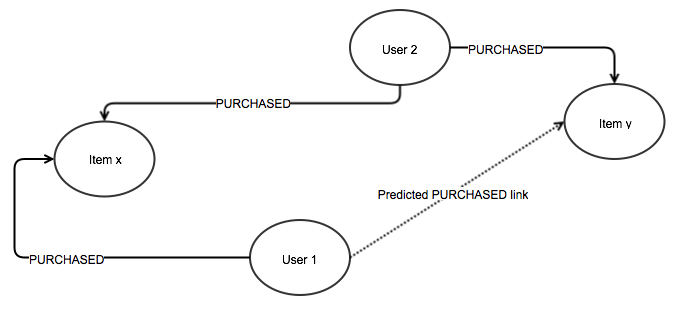
\includegraphics[width=0.75\textwidth]{images/item_link_prediction.png}
  \caption[Item Link Prediction]{Here we see an example of an item recommender system modeled as a graph where the nodes are Users and Items and the edges indicate a purchse of an Item by a User. When modeled this way recommendation takes the form a predicted link in the graph.}
  \label{fig:figures:1}
\end{figure}


\section{User-User Recommender Systems}
There are essentially two types of User-User recommender system algorithms: 1) Similarity based methods and 2) Network based methods.(CITATION NEEDED) Similarity based methods rely on the computation of a user-user similarity metric, which is then used to make recommendations. This is based on the homopholy principle, that users are more likely to be interested in users similar to them. Network based methods analyze the structure of the network to develop recommendations. Example include PageRank, HITS, and SALSA (CITATION NEEDED).

\subsection{Similarity Based Methods}

Collaborative filtering systems produce user specific recommendations based on patterns of behavior observed from other users. Typically this involves observing ratings of items and using either latent factor models or a neighborhood based approach to generate item recommendations\cite{cf}. With the rise of social network analysis however, often instead of user-item recommendations, we are more interested in generating user-user recommendations. User-user recommendations are the focus of this project. The underlying assumption of collaborative filtering is that of homophily: similar users like similar things. Collaborative filtering implementations can be problematic when applied to a large dataset. Most methods require a large sparse matrix for computation, the use of which is not always performant. Instead, the problem can be modeled as a graph, and make use of the graph traversal pattern as an alternative to the construction of a large sparse matrix \cite{Rodriguez}.

\subsection{Network Based Methods}

User-User recommender systems are often generalized as "Who To Follow" recommender systems, as made popular by the "Follow" social network action in the Twitter social network. A Follow action indicates a user expressing interest in another user in the network. This often involves 

The Twitter Who To Follow system is an example of a link prediction system running in production. \cite{wtf} details the design and implementation considerations for such a large scale system. The Twitter system operates on a custom in-memory graph processing engine which implements a PageRank-type algorithm known as Stochastic Approach for Link-Structure Analysis (SALSA). SALSA uses a random walk of the graph to generate link predictions.

\section{Directed Social Networks}
There is an important distinction to note between undirected social networks and directed social networks. Examples/explanation. Much of the literature has focused on undirected social networks only (CITATION NEEDED). In fact the similarity metrics shown above are all based on undirected social networks. A notable exception in the Triadic Closeness method described by (CITATION NEEDED). 

\section{My Approach}
There is a clear gap in the literature making use of combined network based methods with similarity based methods. (CITATION Ensemble paper) My contribution to this field is to explore how these methods can be combined to improve the accuracy of such recommendations. A linear combination of a collaborative filtering similarity based approach and a network based approach levering the use of directed networks is proposed, based somewhat on the work developed in (CITATION paper about novel similarity metric, weighted averaging).
% !TeX encoding=utf8
% !TeX spellcheck = en-US

\chapter{Methods}
Here we describe the data used and detail the implementation. We first examine in detail two methods for link prediction: collaborative filtering using the Jaccard similarity metric and the Triadic Closeness method. We then show how these two methods can be used together in an ensemble predictor using adaptive weights. The data used in this experiment is examined. Finally, implementation is discussed. 

We focus on the link prediction problem for a partially observed network. We assume certain links are missing form the network and attempt to predict the missing link(s), focusing on User-User edges.

\section{Sample Network}
Consider the network shown in figure \ref{thesis_sample_network}. This is a sample network which was randomly generated and does not represent any real world observed data, however we shall refer to this network to demonstrate the techniques used in this project. The sample network contains two types of nodes: Users and Items. Each User can \textit{FOLLOW} other Users. This is represented as a User-User directed edge with the label \textit{:FOLLOWS}. Similarly, Users can express their interest in an Item with the \textit{:LIKES} relationship (or edge). This type of network structure is similar to those observed in social networks (such as Facebook, or Twitter), but also in collaboration networks (such as Github, as we will see in more detail). Since the network has multiple types of nodes and edges it is referred to as a \textbf{multi-modal network}. (CITE GRAPH THEORY / COMPLEX NETWORK BOOK). 

\begin{figure}[H]
  \centering
  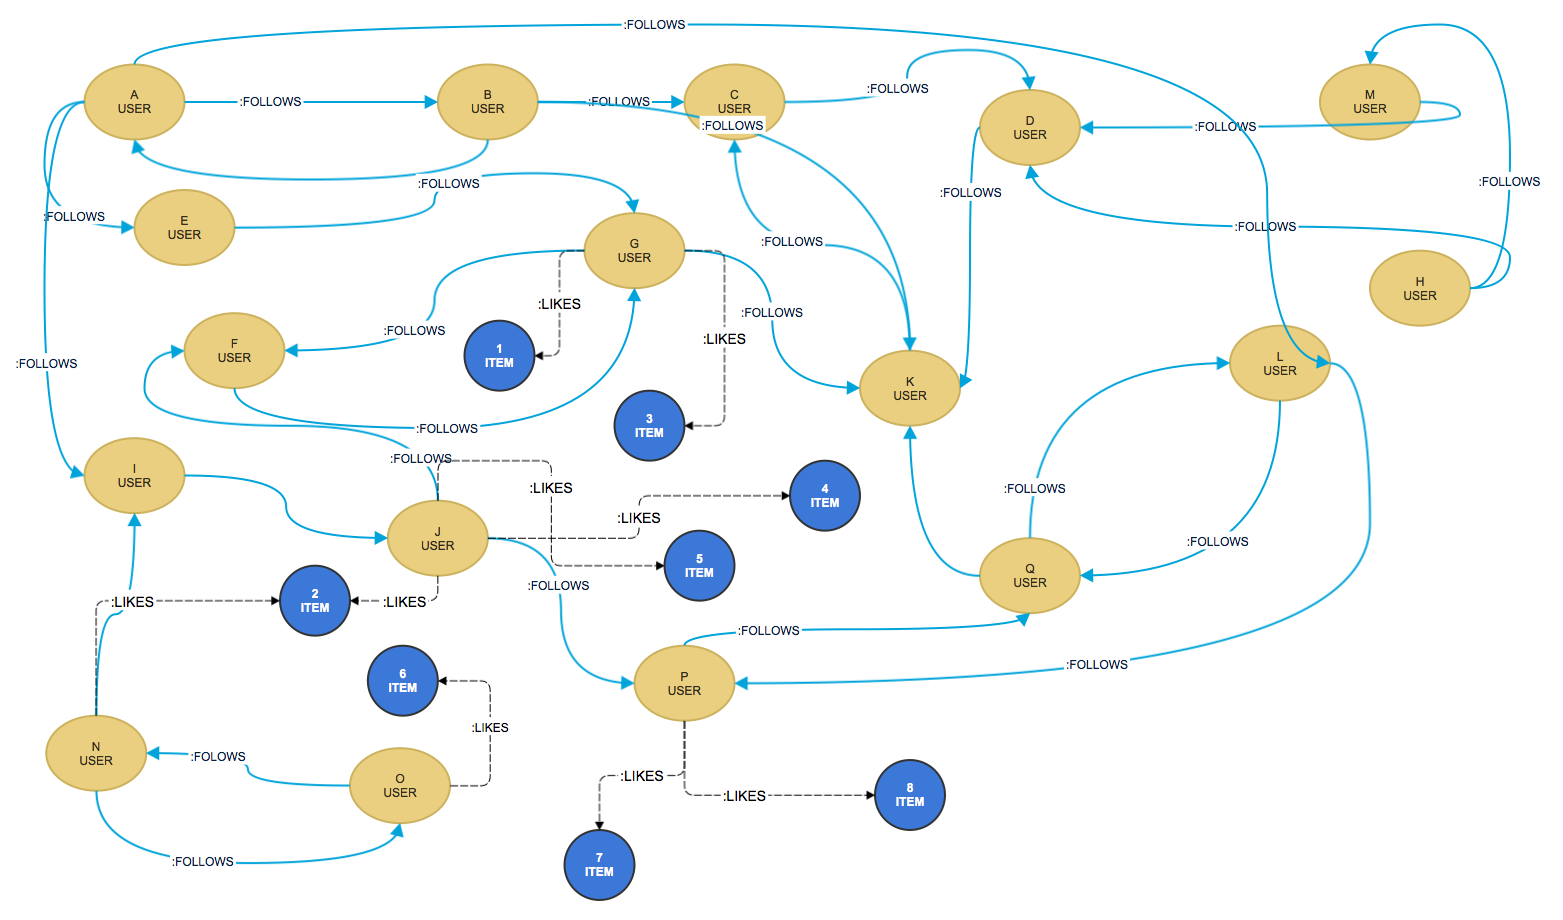
\includegraphics[width=0.75\textwidth]{images/thesis_sample_network_multimodal.png}
  \caption[Sample multi-modal network]{This sample network will be used to demonstrate the methods used for link prediction in this paper. This network demonstrates a random multi-modal network with multiple types of nodes and edges.}
  \label{thesis_sample_network}
\end{figure}

\begin{table}[t]
\caption{Descriptive statistics for sample network}
\label{sample_network_stats}
\vskip 0.15in
\begin{center}
\begin{small}
\begin{sc}
\begin{tabular}{rc}
\hline
Metric & value\\
\hline
Num nodes & 17\\
Num edges & 28\\
Avg degree & 1.67\\
OTHERS & ??\\
\hline
\end{tabular}
\end{sc}
\end{small}
\end{center}
\vskip -0.1in
\end{table}

Some basic descriptive statistics about this sample network are shown in Table \ref{sample_network_stats}. 

\section{Algorithms}

For illustrative purposes we will work through three examples of link prediction algorithms for the sample network shown above. First, using the collaborative filtering method with the Jaccard similarity metric. We will use User-Item edges to identify similar uses and generate recommendations based on those similarities. Next, we walk through the Triadic Closeness method as described in \cite{Schall2014}. Using probabilities observed from triad patterns we will generate link predictions and compare to those created using collaborative filtering. Finaly, we propose a ensemble method that combines collaborative filtering and Triadic Closeness using an adaptive weighting system. In the context of the sample network we focus on predicting User-User \textit{:FOLLOWS} edges only.

For the purposes of the next three sections we will consider link prediction for user J. We proceed through each algorithm manually, ignoring some implementation details for now that will explored in depth in the proceeding section.

\subsection{Collaborative Filtering}
Collaborative filtering is a method of generating recommendations based on the homophily principle: users who are similar are likely to be interested in similar items. It is implemented by finding similar users, based on some similarity metric. \cite{cf} Here we will use User-Item edges as an indication of a User's binary rating of an Item. The Jaccard metric is used to show a proportion of overlapping neighbors

\subsubsection{Similarity Metrics}
The Jaccard index is used to identify similar users. For two users, $a$ and $b$, let $A$ and $B$ denote the sets of all users being followed by $a$ and $b$, respectively. The Jaccard index is therefore as defined in Equation \ref{jaccard}.
\begin{equation}
\label{jaccard}
J(A,B) = \frac{|A \cap B|}{|A \cup B|}
\end{equation}

In this context, Jaccard is defined as the intersection of the Items liked by $a$ and $b$ divided by the union of the items likes by $a$ and $b$. This results in a number between 0 and 1, indicating the strength of similarity between users $a$ and $b$.
 
%\begin{algorithm}[tb]
%
%  \caption{Collaborative Filtering Recommendation}
%   \label{alg:cf}
%\begin{algorithmic}
%   \STATE {\bfseries Input:} Graph $G(V,E)$, vertex $v$, int k
%   
%   \FOR{$i=1$ {\bfseries to} $m-1$}
%   \IF{$x_i > x_{i+1}$} 
%   \STATE Swap $x_i$ and $x_{i+1}$
%   \STATE $noChange = false$
%   \ENDIF
%   \ENDFOR
%  
%\end{algorithmic}
%\end{algorithm}

FIXME: THIS NEEDS TO BE UPDATED FOR NEW DATA MODEL
\begin{algorithm}
\caption{Collaborative filtering algorithm}\label{algo1}
\begin{algorithmic}[1]
\State $input: G(U, E), x, N$ \Comment{explain inputs here}
\State $usersSample \gets getRandomUsers(U,x)$
\State $results \gets \{\}$
\For {$each user in usersSample$}
	\State $validationEdge \gets getRandomEdge(G, user)$
	\State $removeEdge(validationEdge,G)$
	\State fofs $\gets getFOFS(user, G)$
	\State fofRanks $ \gets \{\}$
	\For{each fof in fofs}
		\State j $\gets jaccard(user, fof)$
		fofRanks $\gets results + \{j : fof\}$
	\EndFor
	\State knn $\gets topk(fofRanks, k)$
	\State aggregated $\gets \{\}$
	\For{each kn in knn}
		\State possible $\gets getFollows(kn)$
		\For{each p in possible}
			\If{p in aggregated.keys} $aggregated[p] += 1$ 
				%\State 
			\Else 
				\State $aggregated[p] = 1$
			\EndIf
		\EndFor
	\EndFor
	
	\State $predictions \gets topXSortedByTC(pred, N)$
	\State $hit \gets is validationEdge in predictions?$
	\State $addEdge(validationEdge, G)$
	\State $results \gets results + \{hit, pred, u, v, validation_edge\}$
\EndFor
\State \Return results
\end{algorithmic}
\end{algorithm}

To generate recommendations for user $J$, we first must identify all friend-of-friend nodes, that is nodes that share a neighbor Item in common with $J$. That gives us the set $\{N\}$. Our possible recommendations are now reduced to N. We will now compute the Jaccard similarity metric for the pair $(J, N)$:

\begin{equation}
\label{jaccard}
J(J,N) = \frac{|J \cap N|}{|J \cup N|}
\end{equation}

\begin{equation}
\label{jaccard}
J(J,N) = \frac{|\{Item2\}|}{|\{Item2, Item4, Item5\}|}
\end{equation}

\begin{equation}
\label{jaccard}
J(J,G) = \frac{1}{3}
\end{equation}

We can now predict the edge $J \leftarrow N$ with weight $1/3$. \footnote{If we were interested in predicting User-Item links, we could allow each similar user to \textit{vote} for other Items in which J might have an interest. We now take the top $k$ nodes that have the highest Jaccard score and allow each to vote for new outgoing links to form from $J$. Here we will select $L$ and recommend any outgoing links from $L$ as destination nodes for predicted links emminating from $J$. However, we are only concerned here with User-User edges.}

As you can see, the collaborative filtering link prediction process for a given user $x$ involves finding other users most similar to user $x$, then finding items those similar users are most interested in. In this sense collaborative filtering can be thought of as very similar to k-nearest neighbors, where the distance calculation is based on some similarity metric.

\subsection{Triadic Closeness}
Graph theory proposes the concept of triadic closure, the hypothesis that the creation of an edge between u and v is related to the degree of overlapping neighbors in u and v's respective networks. (CITATION NEEDED and expand on this - see one of the network analysis books I have) The concept of Triadic Closeness is an application of the theory of triadic closure, specifically taking into account the directed nature of social networks. For a given fully observed network, Triadic Closeness can be thought of as the ratio of the number of closed triads to the number of potentially closed triads. \cite{Schall2014}. A triad consists of three nodes $u, z, v$ where edges (ignoring direction) $u,z$ and $z,v$ exist. Edges between $u$ and $v$ may exist, however the concept of triadic closure posits that an implicit connection exists between $u$ and $v$.

\begin{algorithm}
\caption{Triadic Closeness link prediction algorithm}\label{algo_tc}
\begin{algorithmic}[1]
\State $input: G(U, E), x, N$ \Comment{explain inputs here}
\State $usersSample \gets getRandomUsers(U,x)$
\State $results \gets \{\}$
\For {$each user in usersSample$}
	\State $validationEdge \gets getRandomEdge(G, user)$
	\State $removeEdge(validationEdge,G)$
	\State $triads \gets getTriads(user, G)$
	\State $pred \gets \{\}$
	\For {$u, v in triads$}
		\State $tc \gets calcTC(u,v,G)$
		\State $pred \gets pred + \{tc, u, v\}$
	\EndFor
	\State $predictions \gets topXSortedByTC(pred, N)$
	\State $hit \gets is validationEdge in predictions?$
	\State $addEdge(validationEdge, G)$
	\State $results \gets results + \{hit, pred, u, v, validation_edge\}$
\EndFor
\State \Return results
\end{algorithmic}
\end{algorithm}


\begin{figure}[H]
  \centering
  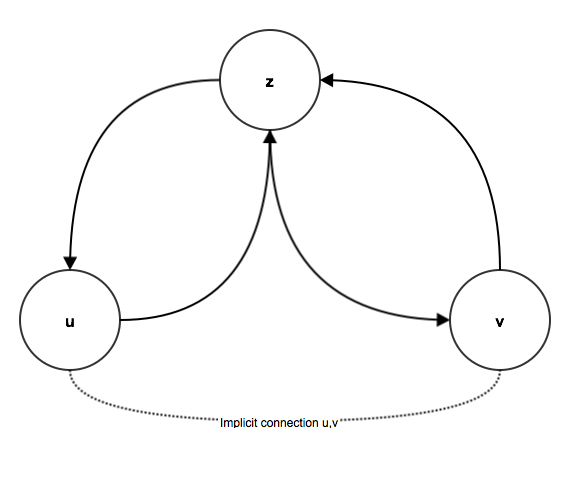
\includegraphics[width=0.4\textwidth]{images/thesis_triad_example.png}
  \caption[closed triad patterns]{A triad is considered to be closed if an edge exists between u and v.}
  \label{thesis_closed_triads}
\end{figure}


In a directed network there are 27 distinct configurations, or patterns that a triad can take on. See (CITATION TABLE of triad patterns). Table \ref{sample_network_freq} shows triad patterns that are open, that is no connection exists between nodes $u$ and $v$. The pattern identifications $(T01, T02...)$ are taken from (CITE PROPERLY) Schall 2013. Any open triad can be closed in one of three possible ways: $u \leftarrow v$, $u \rightarrow v$, or $u \leftrightarrow v$.

INSERT IMAGE OF 3 CLOSED TRIAD PATTERNS 
\begin{figure}[H]
  \centering
  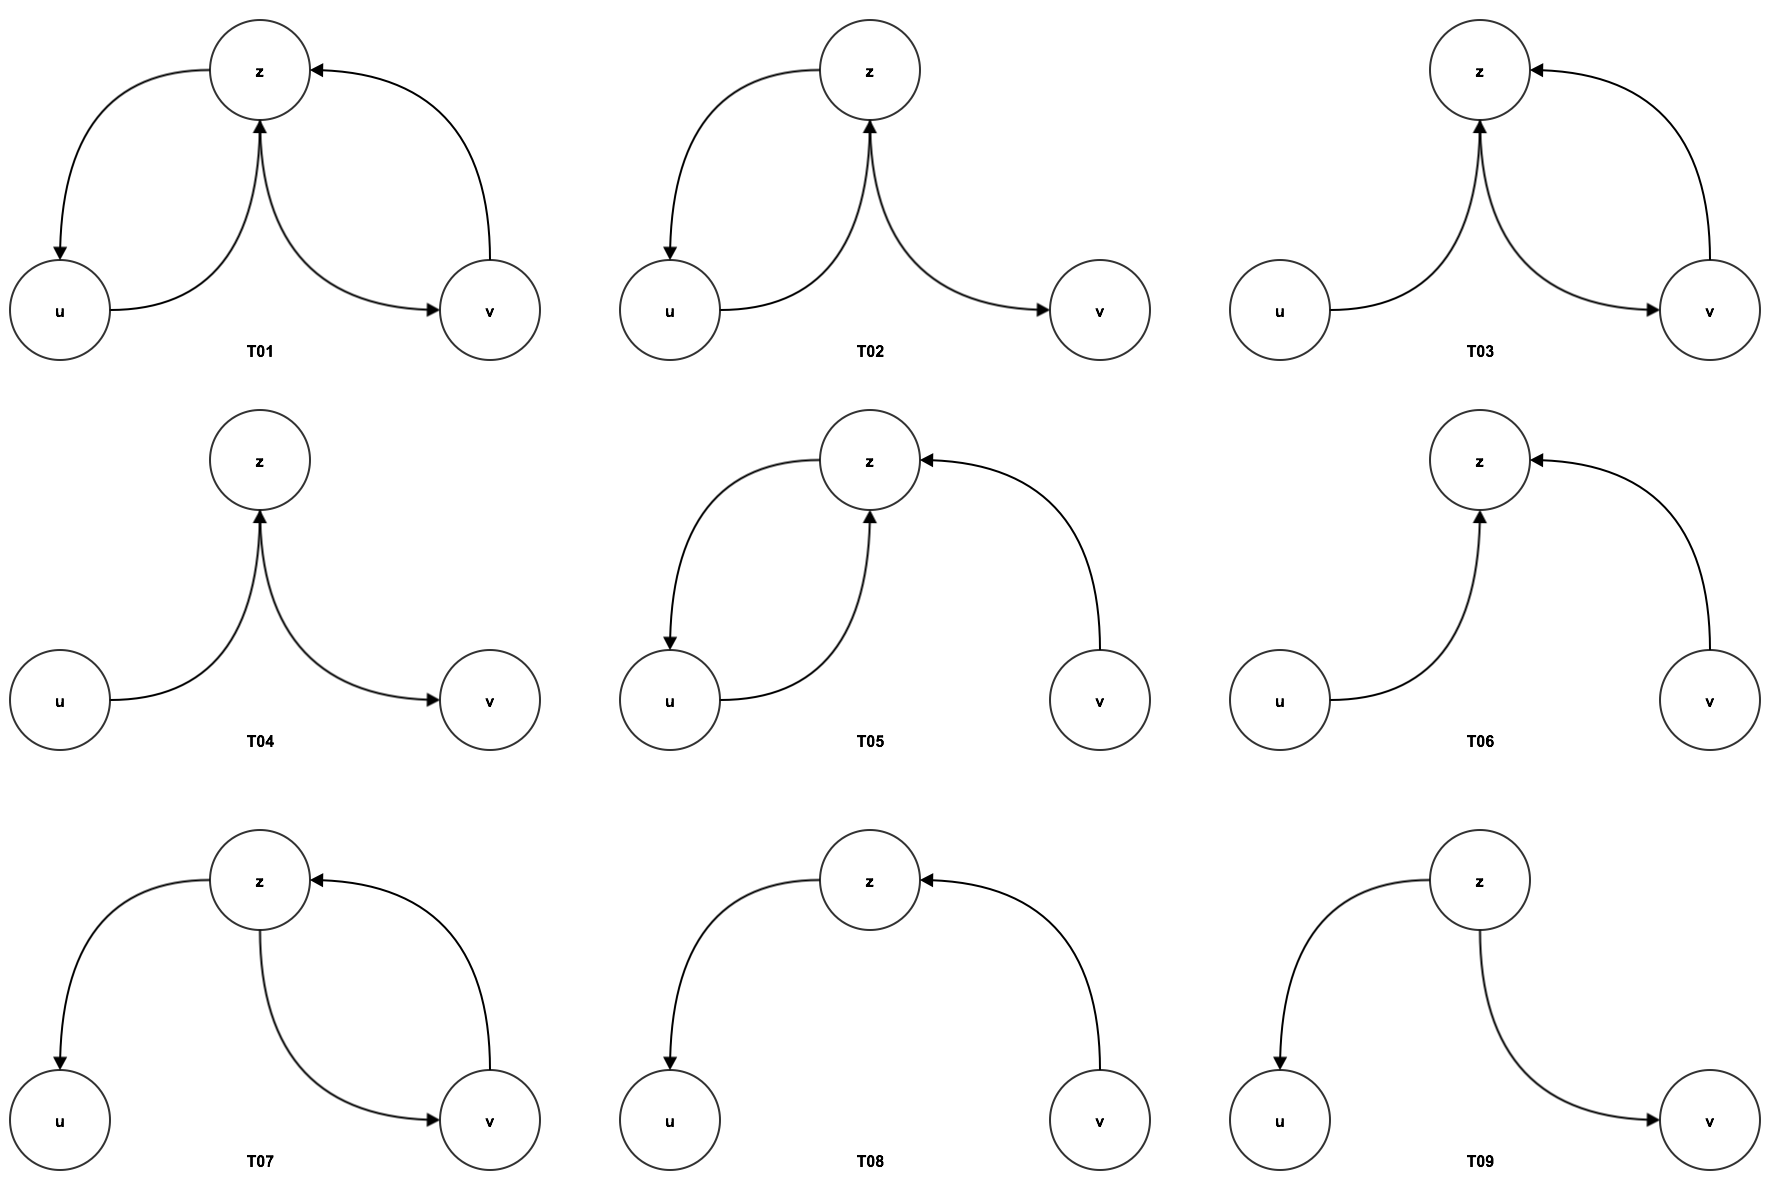
\includegraphics[width=0.75\textwidth]{images/thesis_triad_patterns.png}
  \caption[triad patterns]{All possible open triad patterns are shown. A triad is said to be closed is a connection is established between u and v.}
  \label{thesis_triad_patterns}
\end{figure}

\begin{figure}[H]
  \centering
  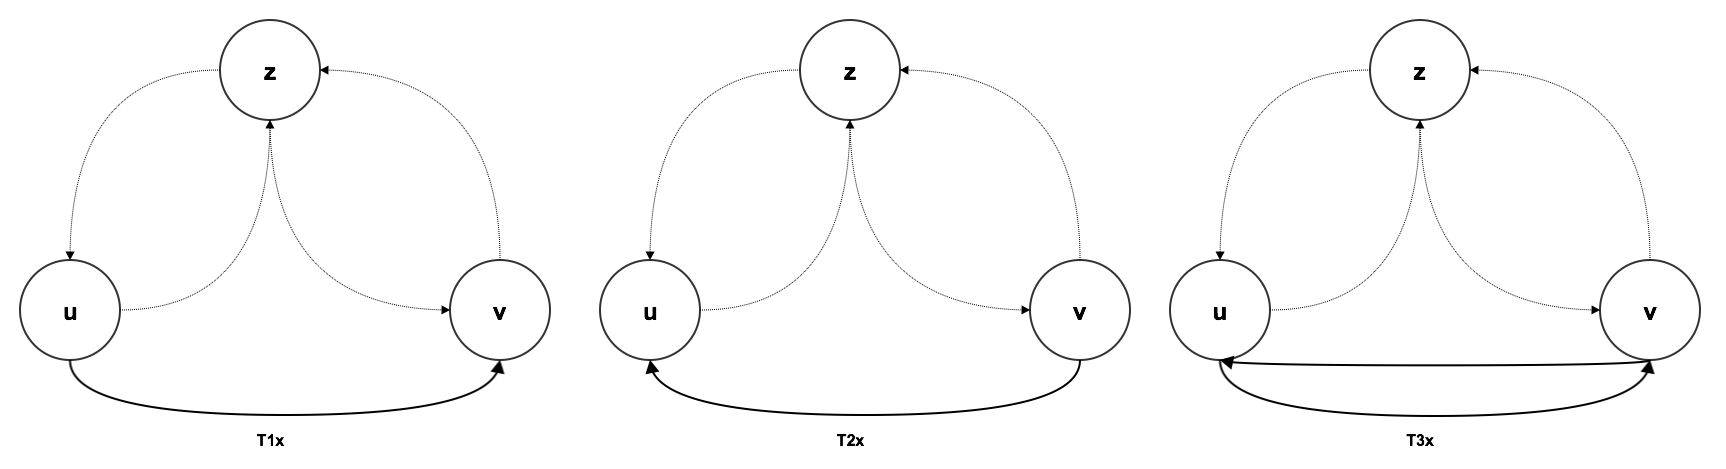
\includegraphics[width=0.75\textwidth]{images/thesis_closed_triads.png}
  \caption[closed triad patterns]{A triad is considered to be closed if an edge exists between u and v.}
  \label{thesis_closed_triads}
\end{figure}

Figure \ref{thesis_closed_triads} shows the three distinct ways in which an open triad can be closed. Either the creation of an edge $u \rightarrow u$, the creation of an edge $u \leftarrow v$, or the creation of two edges $u \rightarrow v$ and $u \leftarrow v$. In terms of the triad pattern id, the first digit indicates if the triad is open (0), closed with an edge $u \rightarrow v$ (1), closed with an edge $u \leftarrow v$ (2), or closed with two edges $u \rightarrow v$ and $u \leftarrow v$ (3). With this nomenclature we are now able to represent each possible triad pattern with a two digit identifier. 

\begin{table}[t]
\caption{Open triad pattern frequency in the sample network shown in Figure CITATION NEEDED}
\label{sample_network_freq}
\vskip 0.15in
\begin{center}
\begin{small}
\begin{sc}
\begin{tabular}{rrccr}
\hline
ID & Pattern & Count \\
\hline
T06 & $u \rightarrow z \leftarrow v $ & 20 \\
T04 &$ u \rightarrow z \rightarrow v$ & 14 \\
T08 & $u \leftarrow z \leftarrow v$ & 14 \\
T02 & $u \leftrightarrow z \rightarrow v$ & 8 \\
T07 & $u \leftarrow z \leftrightarrow v$ & 8 \\
T09 & $u \leftarrow z \rightarrow v$ & 8 \\
T03 & $u \rightarrow z \leftrightarrow v$ & 3 \\
T05 & $u \leftrightarrow z \leftarrow v$ & 3 \\

\hline
\end{tabular}
\end{sc}
\end{small}
\end{center}
\vskip -0.1in
\end{table}

\begin{table}[t]
\caption{Closed triad pattern frequency in the sample network shown in Figure CITATION NEEDED}
\label{sample_network_freq}
\vskip 0.15in
\begin{center}
\begin{small}
\begin{sc}
\begin{tabular}{rrccr}
\hline
ID & Pattern & Count \\
\hline
T18 & $u \leftarrow z \leftarrow v \leftarrow u$ & 3 \\
T14 & $u \rightarrow z \rightarrow v \leftarrow u$ & 2 \\
T16 & $u \rightarrow z \leftarrow v \leftarrow u$ & 2 \\
T19 & $u \leftarrow z \rightarrow v \leftarrow u$ & 2 \\
T15 & $u \leftrightarrow z \leftarrow v \leftarrow u$ & 1 \\
T17 & $u \leftarrow z \leftrightarrow v \leftarrow u$ & 1 \\
T24 & $u \rightarrow z \rightarrow v \rightarrow u$ & 3 \\
T26 & $u \rightarrow z \leftarrow v \rightarrow u$ & 2 \\
T28 & $u \leftarrow z \leftarrow v \rightarrow u$ & 2 \\
T29 & $u \leftarrow z \rightarrow v \rightarrow u$ & 2 \\
T22 & $u \leftrightarrow z \rightarrow v \rightarrow u$ & 1 \\
T23 & $u \rightarrow z \leftrightarrow v \rightarrow u$ & 1 \\
T34 & $u \rightarrow z \rightarrow v \leftrightarrow u$ & 1 \\
T38 & $u \leftarrow z \leftarrow v \leftrightarrow u$ & 1 \\
\hline
\end{tabular}
\end{sc}
\end{small}
\end{center}
\vskip -0.1in
\end{table}

\begin{equation}
TC_{uv} = \sum_{z\in \Gamma(u)\cap \Gamma(v)} w^{P}(u, v, z) \times w(z)  
\end{equation}

\begin{equation}
w^{P}(u,v,z) = \frac{F(T(u,v,z) + 10) + F(T(u,v,z) + 30)}{F(T(u,v,z))}
\end{equation}

\begin{equation}
TC_{uv} = \sum_{z\in \Gamma(u)\cap \Gamma(v)} w^{P}(u,v,z) \times \frac{1}{k_z}
\end{equation}

Having collected these triad pattern frequencies, we can now generate recommendations as we did in section (REFERENCE SECTION COLLABORATIVE FILTERING) for user $J$.

The first step is identify all open triads of the form u,z,v where J is u and no link between u,z exists. Those triads are:

(J,F,G),\\
(J,I,N), \\ 
(J,P,Q)

(INSERT GRAPH HERE OF THE THREE TRIADS AND THEIR PATTERNS)

Thus the three possible recommendations that we might generate are $J \rightarrow G$, $J \rightarrow N$, and $J \rightarrow Q$. To determine the rank of the predictions, we must calculate the triadic closeness metric for the pairs $(J,G)$, $(J,N)$ and $(J,A)$. 

\begin{equation}
TC_{JG} = \sum_{z\in \Gamma(J)\cap \Gamma(G)} w^{P}(J, G, z) \times w(z)  
\end{equation}

\begin{equation}
TC_{JG} = w^{P}(J, G, F) \times w(F)  
\end{equation}

\begin{equation}
w^{P}(J,G,F) = \frac{F(T(J,F,G) + 10) + F(T(J,F,G) + 30)}{F(T(J,F,G))}
\end{equation}

We can see that T(J,F,G) = T03, so we have:

\begin{equation}
w^{P}(J,G,F) = \frac{F(T03 + 10) + F(T03 + 30)}{F(T03)}
\end{equation}

\begin{equation}
w^{P}(J,G,F) = \frac{0 + 0}{3}
\end{equation}

\begin{equation}
w^{P}(J,G,F) = 0
\end{equation}

\begin{equation}
TC_{JG} = 0
\end{equation}

Next for J,N:

\begin{equation}
TC_{JG} = \sum_{z\in \Gamma(J)\cap \Gamma(G)} w^{P}(J, N, z) \times w(z)  
\end{equation}

\begin{equation}
TC_{JG} = w^{P}(J, I, N) \times w(I)  
\end{equation}

\begin{equation}
w^{P}(J,G,F) = \frac{F(T(J,I,N) + 10) + F(T(J,I,N) + 30)}{F(T(J,I,N))}
\end{equation}

We can see that T(J,I,N) = T08, so we have:

\begin{equation}
w^{P}(J,G,F) = \frac{F(T08 + 10) + F(T08 + 30)}{F(T08)}
\end{equation}

Using table (TRIAD FREQ PATTERN REF TABLE)

\begin{equation}
w^{P}(J,G,F) = \frac{3 + 1}{14}
\end{equation}

\begin{equation}
w^{P}(J,G,F) = 0.286
\end{equation}

\begin{equation}
w(I)=1/3
\end{equation}

\begin{equation}
TC_{JN} = 0.286 \times 1/3 = 0.095
\end{equation}


and finally, calculate TC(J,Q):


\begin{equation}
TC_{JQ} = \sum_{z\in \Gamma(J)\cap \Gamma(Q)} w^{P}(J, Q, z) \times w(z)  
\end{equation}

\begin{equation}
TC_{JG} = w^{P}(J, P, A) \times w(Q)  
\end{equation}

\begin{equation}
w^{P}(J,P,Q) = \frac{F(T(J,P,Q) + 10) + F(T(J,P,Q) + 30)}{F(T(J,P,Q))}
\end{equation}

We can see that T(J,P,Q) = T04, so we have:

\begin{equation}
w^{P}(J,P,Q) = \frac{F(T04 + 10) + F(T04 + 30)}{F(T04)}
\end{equation}

\begin{equation}
w^{P}(J,P,Q) = \frac{2 + 0}{14}
\end{equation}

\begin{equation}
w^{P}(J,P,Q) = 0.143
\end{equation}

\begin{equation}
w(P)=1/3
\end{equation}

\begin{equation}
TC_{JQ} = 0.143 \times 1/3
\end{equation}

\begin{equation}
TC_{JQ} = .048
\end{equation}

We can then sort our recommendations by TC and the most likely edge we will recommend is $J \rightarrow Q$.

\subsection{An adaptive ensemble method}
Each of the two methods described above do not fully capture the information needed to make robust recommendations:
\begin{itemize}
\item Collaborative filtering captures similar items to identify nodes that a user might find interesting, however the model does not capture any probabilistic information to inform how likely the link is to form, given the relevant/similar node.
\item While Triadic Closeness captures probabilistic information that informs how likely certain triad patterns are to close, it is not informed by any user rating observations. This results in predictions based solely on patterns and ignoring content similarity.
\end{itemize}

We next examine how these two methods can be combined to improve link prediction. \cite{Lu2010} identifies such hybrid methods as a way to improve accuracy of link prediction beyond what any one algorithm might be able to obtain.

While such an ensemble method could be defined as a simple weighted average with fixed weights as described in \cite{Candillier}, we instead propose an adaptive weighting mechanism to take into account the information available for each component of the ensemble metric. 

Consider: 
\begin{equation}
AEM_{u,v} = \sum_{c \in components} c(u, v) \times w_c(u,v)  
\end{equation}

Using Jaccard and Triadic Closeness, this becomes:

\begin{equation}
AEM_{u,v} = J(u,v) \times w_J(u,v) + TC(u,v) \times w_{TC}(u,v)
\end{equation}

Both Jaccard and Triadic Closeness metrics are in the range \{0,1\} so we do not need to normalize.  $J(u,v)$ is described above in Equation XX and $TC(u,v)$ in Equation XX, but what values to assign the weights $w_J$ and $w_{TC}$? Rather than assigning equal weights, the weights should be assigned according to the proportion of our confidence in each metric. Since we are dealing with a multi-modal network, each metric is calculated using a certain relationship type. Here Jaccard is calculated using User-Item \textit{:LIKES} relationships, while Triadic Closeness is calculated using only User-User \textit{:FOLLOWS} relationships. For a given user, $u$ we can use the proportion of total out-edges of each relationship type as the weight for the corresponding metric.

For example:

\begin{equation}
w_J(u,v) = \frac{count(u-\{:LIKES\}->)}{count(u-\{*\}->)}
\end{equation}

\begin{equation}
w_{TC} = \frac{count(u-\{:FOLLOWS\}->)}{count(u-\{*\}->)}
\end{equation}

Where $count(u-\{:LIKES\}->)$ is the number of outgoing \textit{:LIKES} edges for User $u$ and $count(u-\{*\}->)$ is the total number of outgoing edges (both \textit{:LIKES} and \textit{:FOLLOWS}).  

We can think of each outgoing edge as a rating or vote from that user, expressing their interest. If for a given user we observe 10 \textit{:FOLLOWS} edges and only 1 \textit{:LIKES} edge, we have greater confidence in the accuracy of the Triadic Closeness metric since we have more information about User $u$'s preferences. 

\section{Implementation}

\begin{figure}[ht]
\vskip 0.2in
\begin{center}
\centerline{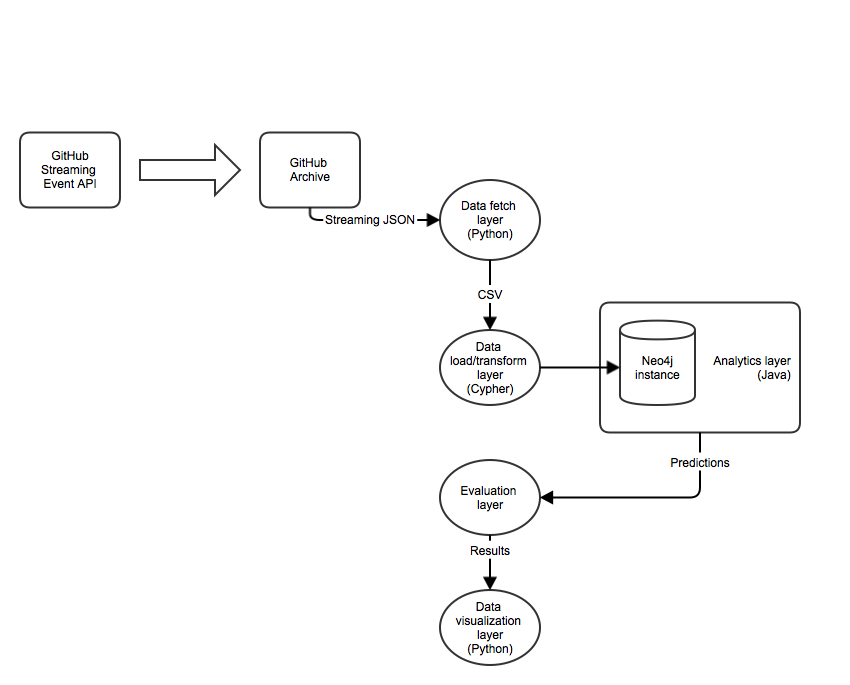
\includegraphics[width=0.75\columnwidth]{images/thesis_architecture.png}}
\caption[Link prediction system architecture]{The GitHub follow graph is a simple graph with User nodes and Follows edges.}
\label{github_simplified_data_model}
\end{center}
\vskip -0.2in
\end{figure} 


We implement a system capable of generating recommendations using each of the three methods described above (Jaccard similarity, Triadic Closeness, and an adaptive ensemble method). This system is written in Java and makes use of the Neo4j graph database.

\subsection{Graph Data Model}
We model the data as a graph, $G = (V, E)$ 

\subsection{Graph Traversal Pattern}
The graph traversal pattern allows us to design algorithms where the answer to our question is a traversal through the graph. 

\subsection{Graph Database And Querying Traversals}
Why using a graph database makes sense.
Performance benefits of using graph database.
Compare to how this would be modeled in a RDBMS or a document DB.

\subsection{Triad detection}

%\label{sec:example:code}
%
%\ifcsdef{lstStyleLaTeX}{%
%  \lstinputlisting[style=lstStyleLaTeX,%nolol=true,%
%     caption={LaTeX Typesetting By Example}, label=lstLaTeXExample]  
%  {content/demo/latextutorial.tex}
%}{}


Triad detection involves scanning the entire graph to identify triads in the network, both open and closed.

%\subsection{Steps}
%The following describes implementation of the system at a high level. For each validation fold:
%
%\begin{itemize}
%\item Select $p$ users at random
%\item For each user $u$ in $p$:
%	\begin{itemize}
%	\item Remove one $FOLLOWS$ edge $f$ for this user at random
%	\item Find $k$ nearest neighbors using Jaccard index (ensure removed edge is not used for this calculation)
%	\item Calculate $n$ followed users with greatest overlap (the most commonly followed users among the $k$ nearest neighbors)
%	\item Return set of $n$ users, these are the recommended users
%	\item Is $f$ in $n$? If yes, this run is counted as a valid prediction.
%	\end{itemize}
%\item Report summary accuracy metrics for this fold
%\end{itemize}


%caption{Collaborative Filtering Recommendation}
%\label{alg:cf}

\section{Data}


\begin{figure}[H]
  \centering
  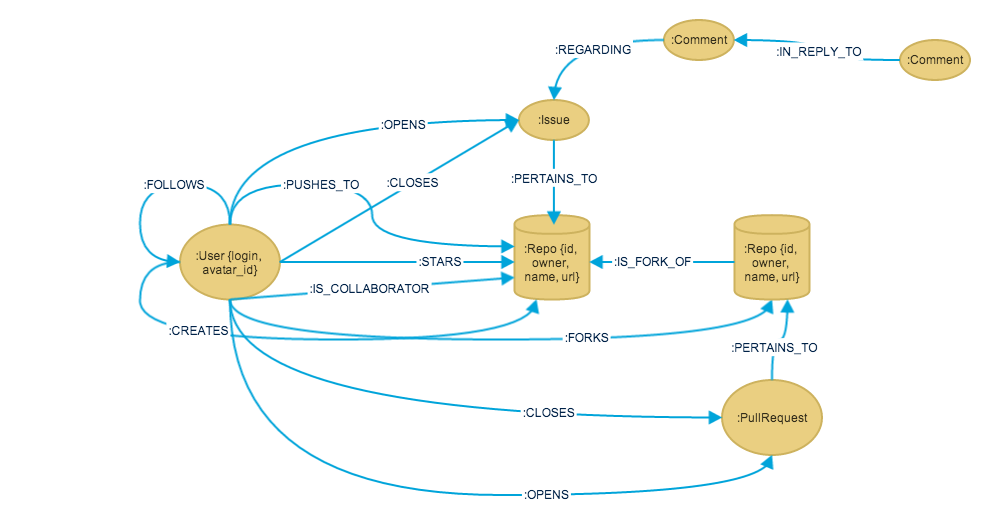
\includegraphics[width=0.75\textwidth]{images/githubdatamodel.png}
  \caption[GitHub graph data model]{GitHub data model as a labeled property graph.}
  \label{github_data_model}
\end{figure}

GitHub \footnote{\url{http://github.com}} is an online social collaboration network built around the Git version control system. GitHub allows software developers to share and collaborate on software projects. Many open-source software projects are hosted on GitHub and use GitHub as their primary development and distribution platform. GitHub also has a social component: users are able to \textit{follow} other users to receive updates about user activity. This combination of social and collaboration components make GitHub an excellent example of a multi-modal complex network. 


\begin{figure}[ht]
\vskip 0.2in
\begin{center}
\centerline{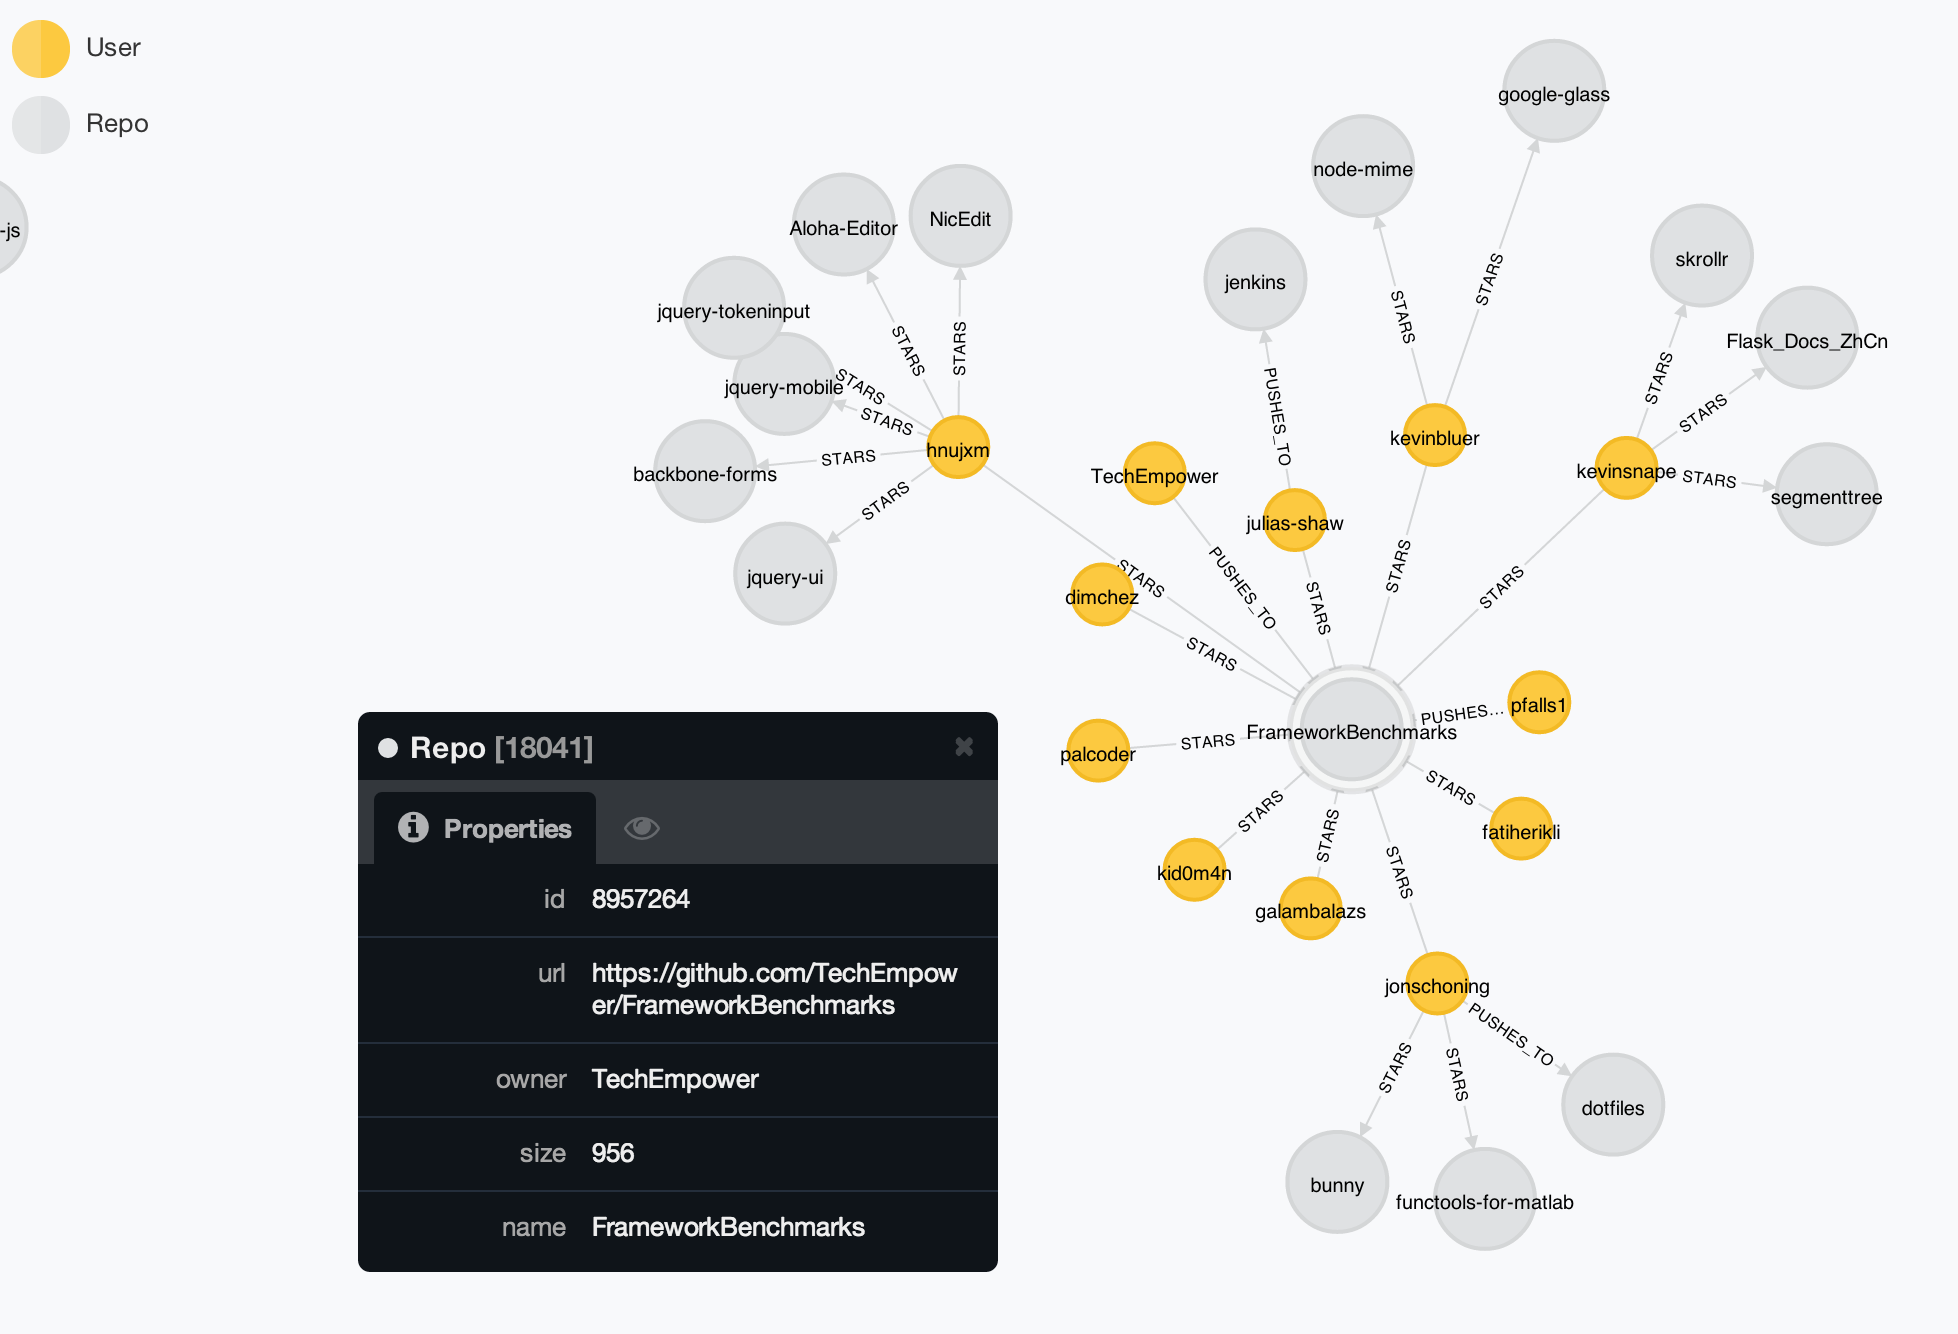
\includegraphics[width=0.75\columnwidth]{images/neo_screenshot.png}}
\caption{GitHub data model as a property graph. Screenshot from Neo4j graph database interface.}
\label{screenshot-data}
\end{center}
\vskip -0.2in
\end{figure} 


The GitHub network is multi-modal in that there are multiple nodes types (primarily Users and Repositories, or software projects) and multiple edge types (User-User follows, User-Repository Stars, etc). Figure \ref{github_data_model} shows a portion of the GitHub data modeled as a graph. This data model is quite rich, however for the purposes of this paper we will only concern ourselves with User-User \textit{:FOLLOWS} and User-Repository \textit{:STARS} edges. That simplifies the data model to that shown in Figure \ref{github_simplified_data_model}.


\begin{figure}[ht]
\vskip 0.2in
\begin{center}
\centerline{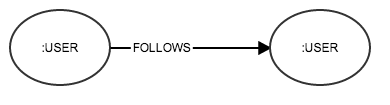
\includegraphics[width=0.3\columnwidth]{images/user_user.png}}
\caption[User-User data model]{The GitHub follow graph is a simple graph with User nodes and Follows edges.}
\label{github_simplified_data_model}
\end{center}
\vskip -0.2in
\end{figure} 

\subsection{Github Archive}
Data was collected from GitHub Archive\cite{githubarchive}, a service that maintains an archive of all public events emitted by the GitHub API\cite{github:Online}. These include events such as creation of new repositories, pushes to repositories, repository stars, and user follows. Data was collected for the time period April 1st, 2013 - April 1st, 2014. For the purposes of this project, only \textit{FOLLOWS} events were considered. This resulted in a total of 539893 users and 919489 follows. In terms of a graph, that equates to 539893 nodes and 919489 vertices between nodes.

A graph data model is used to represent this data as the data is highly connected: it is describing entities (users and repositories) and their interactions (stars, follows, pushes, etc). Figure \ref{screenshot-data} shows an example of a subgraph of user and repository nodes and the interactions among those entities, modeled as a graph.

\subsubsection{FollowEvent}
\begin{lstlisting}[style=lstStyleCpp, caption={LaTeX Typesetting By Example}, label=lstLaTeXExample]
{
  "created_at": "2013-07-11T15:03:05-07:00",
  "payload": {
    "target": {
      "id": 4602587,
      "login": "smarquez1",
      "followers": 1,
      "repos": 1,
      "gravatar_id": "42eb6556201588fa7641bf2f0bf615e6"
    }
  },
  "public": true,
  "type": "FollowEvent",
  "url": "https://github.com/smarquez1",
  "actor": "matiasalvarez87",
  "actor_attributes": {
    "login": "matiasalvarez87",
    "type": "User",
    "gravatar_id": "0ee1a5bec013545c91ad05c451fb9715",
    "name": "Matias Alvarez Duran",
    "company": "NaN Labs",
    "blog": "http://ar.linkedin.com/pub/matias-emiliano-alvarez-duran/17/39b/a96",
    "location": "Argentina",
    "email": "matiasalvarez87@gmail.com"
  }
}
\end{lstlisting}

\subsubsection{WatchEvent (Stars)}
\begin{lstlisting}[style=lstStyleCpp, caption={peep this JSON object dawg},
label=watchEventListing]
{
  "created_at": "2013-07-11T15:01:56-07:00",
  "payload": {
    "action": "started"
  },
  "public": true,
  "type": "WatchEvent",
  "url": "https://github.com/CamDavidsonPilon/Probabilistic-Programming-and-Bayesian-Methods-for-Hackers",
  "actor": "cebe",
  "actor_attributes": {
    "login": "cebe",
    "type": "User",
    "gravatar_id": "2ebfe57beabd0b9f8eb9ded1237a275d",
    "name": "Carsten Brandt",
    "company": "cebe.cc",
    "blog": "http://cebe.cc/",
    "location": "Berlin, Germany",
    "email": "mail@cebe.cc"
  },
  "repository": {
    "id": 7607075,
    "name": "Probabilistic-Programming-and-Bayesian-Methods-for-Hackers",
    "url": "https://github.com/CamDavidsonPilon/Probabilistic-Programming-and-Bayesian-Methods-for-Hackers",
    "description": "aka \"Bayesian Methods for Hackers\": An introduction to Bayesian methods + probabilistic programming with a computation/understanding-first, mathematics-second point of view. All in pure Python ;)  ",
    "homepage": "http://camdavidsonpilon.github.io/Probabilistic-Programming-and-Bayesian-Methods-for-Hackers",
    "watchers": 3353,
    "stargazers": 3353,
    "forks": 444,
    "fork": false,
    "size": 1264,
    "owner": "CamDavidsonPilon",
    "private": false,
    "open_issues": 21,
    "has_issues": true,
    "has_downloads": true,
    "has_wiki": true,
    "language": "Python",
    "created_at": "2013-01-14T07:46:28-08:00",
    "pushed_at": "2013-07-04T17:08:47-07:00",
    "master_branch": "master"
  }
}
\end{lstlisting}





\subsection{Data Analysis}

Table \ref{dataset_stats} shows some descriptive statistics about the GitHub dataset used for this project. The observed network consists of 1.7 million nodes (this includes both Users and Repositories) and 10.7 million edges (both User-User $follows$ edges and User-Repository $stars$ edges. 


\begin{table}[ht]
\centering
\small\renewcommand{\arraystretch}{1.4}  
\rowcolors{1}{tablerowcolor}{tablebodycolor}
%
\captionabove[GitHub network descriptive statistics]{Here we see the most "central" Users per their PageRank rankings. This is based on the graph created by user-user follows edges.}
\label{dataset_stats}
\begin{tabularx}{0.7\textwidth}{lXXX}
\hline
\rowcolor{tableheadcolor}
 & Count \\
\hline
Num nodes &   1,751,605 \\
Num edges & 10,740,463 \\
Mean degree & 6.13 \\
Num $USER$ nodes & 871,382  \\
Num $REPO$ nodes &  880,223\\
Num $:FOLLOWS$ edges & 1,120,069 \\
Num $:STARS$ edges & 9,620,394 \\
Mean $:FOLLOWS$ degree & 1.29 \\
Mean $:STARS$ degree & 11.04 \\
\hline
\hline
\end{tabularx}
\end{table}

As an initial sanity check for exploring the data we compute PageRank for the observed GitHub network. PageRank is a link analysis algorithm that assigns weights to nodes in a network based on that nodes relative importance, or centrality in the network. \cite{pagerank} It is similar to a measure of eigenvector centrality. PageRank has the weakness of only being applicable to a homogenous or single mode network, therefore we apply the algorithm to the User-User $follows$ subgraph and the User-Repository $stars$ subgraph separately. The GraphLab PageRank algorithm implementation is used \cite{GraphLab}.

\begin{table}[ht]
\centering
\small\renewcommand{\arraystretch}{1.4}  
\rowcolors{1}{tablerowcolor}{tablebodycolor}
%
\captionabove[PageRank for User-User follows]{Here we see the most "central" Users per their PageRank rankings. This is based on the graph created by user-user follows edges.}
\label{follow_pagerank_table}
%
\begin{tabularx}{0.4\textwidth}{lXXX}
\hline
\rowcolor{tableheadcolor}
User & PageRank \\
\hline
funkenstein& 413.14 \\
mojombo & 300.01 \\
torvalds & 248.21 \\
rippleFoundation & 220.29 \\
visionmedia & 140.52 \\
paulirish & 129.59 \\
BYVoid & 114.29 \\
schacon & 112.17 \\
JakeWharton & 110.55 \\
defunkt & 106.86 \\
mattt & 99.38 \\
worrydream & 87.33 \\
hakimel & 83.05 \\
pjhyett & 80.89 \\
addyosmani & 80.59 \\
mbostock & 75.63 \\
mdo & 70.40 \\
LeaVerou & 66.92 \\
tekkub & 62.24 \\
nf & 60.93 \\
\hline
\end{tabularx}
\end{table}




\begin{table}[ht]
\centering
\small\renewcommand{\arraystretch}{1.4}  
\rowcolors{1}{tablerowcolor}{tablebodycolor}
%
\captionabove[PageRank for User-Repository stars]{Top 20 central GitHub repositories by PageRank.}
\label{star_pagerank_table}
%
\begin{tabularx}{0.8\textwidth}{lXXX}
\hline
\rowcolor{tableheadcolor}
Repository & PageRank \\
\hline
\url{https://github.com/vhf/free-programming-books} & 455.07 \\
\url{https://github.com/twbs/bootstrap} & 335.46 \\
\url{https://github.com/jquery/jquery} & 289.42 \\
\url{https://github.com/resume/resume.github.com} & 251.99 \\
\url{https://github.com/mandatoryprogrammer/Octodog} & 233.41 \\
\url{https://github.com/angular/angular.js} & 202.18 \\
\url{https://github.com/mbostock/d3} &149.55 \\
\url{https://github.com/torvalds/linux} & 133.48 \\
\url{https://github.com/FortAwesome/Font-Awesome} & 121.47 \\
\url{https://github.com/twitter/bootstrap} & 111.42 \\
\url{https://github.com/laravel/laravel} & 106.75 \\
\url{https://github.com/papers-we-love/papers-we-love} & 102.25 \\
\url{https://github.com/joyent/node} &101.27 \\
\url{https://github.com/rethinkdb/rethinkdb} & 92.34 \\
\url{https://github.com/neovim/neovim} & 91.52 \\
\url{https://github.com/libgit2/libgit2} & 90.99 \\
\url{https://github.com/rogerwang/node-webkit} & 88.23 \\
\url{https://github.com/github/gitignore} & 88.08 \\
\url{https://github.com/dypsilon/frontend-dev-bookmarks} & 86.73 \\
\url{https://github.com/zurb/foundation} & 84.25 \\
\hline
\end{tabularx}
\end{table}

Tables \ref{follow_pagerank_table} and \ref{star_pagerank_table} show the highest ranked Users and Repositories for the GitHub data collected. 

Table \ref{follow_pagerank_table} shows the results of the PageRank algorithm using User-User $follows$ relationships only. As a sanity check of the data, we expect the highest ranked Users to be influential develops in the open-source software development community - the nodes with highest relative importance in this context. A cursory evaluation of the list of GitHub usernames confirms that this is indeed the case: 

\begin{description}
\item [mojombo] Tom Preston-Werner, a co-founder and developer of GitHub
\item [torvalds] Linus Torvalds, maintainer of the linux operating system kernel
\item [paulirish] Paul Irish, a well known Google developer
\item [mbostock] Mike Bostock, core developer of d3.js a popular JavaScript data visualization library
\item [mdo] Mark Otto, one of the developers of Bootstrap the widely used frontend CSS/Javascript framework
\end{description}

Similarly, Table \ref{stars_pagerank_table} enumerates the 20 most central GitHub software repositories, according to PageRank. Here we expect  


% !TeX encoding=utf8
% !TeX spellcheck = en-US

\chapter{Evaluation}

The result of the algorithm is a set of user ids that are predicted destination nodes, given a specific source node. These are recommended users that the specified user might be interested in following. 
\begin{table}[t]
\caption{Evaluation metrics for cross fold validation runs with varying parameters. K is number of neighbors allowed to vote. N is number of predicted links. Precision and accuracy are evaluation metrics, expressed in percentages. Random is the probability of at least one of the N links being relevant if N links are chosen at random.}
\label{results}
\vskip 0.15in
\begin{center}
\begin{small}
\begin{sc}
\begin{tabular}{rrccr}
\hline
k & n & Precision (\%) & Accuracy (\%) & Random (\%) \\
\hline
5      & 25 & 0.61 & 15.0 & 0.0046\\
5      & 50 & 0.18 & 8.0 & 0.0093 \\
5      & 100&0.19 & 15.0 & 0.0185\\
10    & 25 & 0.16& 4.0 & 0.0046\\
10    & 50 & 0.14 & 7.0 & 0.0093\\
10    & 100&0.19 & 18.0 & 0.0185 \\
25    & 25 & 0.24 & 6.0  & 0.0046\\
25    & 50 & 0.12 & 6.0  & 0.0093\\
25    &100&0.11 & 11.0  & 0.0185\\  
50    & 25 &0.12 & 3.0 & 0.0046\\
50    & 50 & 0.14 & 7.0  & 0.0093\\
50    &100& 0.10 & 0.10  & 0.0185\\
100 & 25 & 0.28 & 7.0  & 0.0046\\
100 & 50 & 0.16 & 8.0  & 0.0093\\
100 &100& 0.05 & 5.0  & 0.0185\\
1000&25&0.32 & 8.0  & 0.0046\\
1000&50&0.24& 12.0  & 0.0093\\
1000&100&0.14&14.0  & 0.0185\\
2000&25&0.24&6.0 & 0.0046\\
2000&50&0.18&9.0 & 0.0093\\
2000&100&0.10&10.0  & 0.0185\\
\hline
\end{tabular}
\end{sc}
\end{small}
\end{center}
\vskip -0.1in
\end{table}

\subsection{Evaluation}
The system is evaluated using several iterations for cross-validation with different configurations. Table \ref{results} shows the results. Two methods of evaluation are identified as the standard for evaluating link prediction systems: precision and area under the receiver operating characteristic curve (AUC). Precision is defined as the ratio of the relevant items selected to the total number of items selected. AUC is a more involved calculation that requires an all-pairs comparison of the rank of the predicted link and {\textit all other possible unobserved links in the network}. Due to the size of the GitHub network, calculating this metric was not seen as feasible. Instead of AUC, a simple accuracy metric is calculated: if the removed link is present in the array of predicted links we count the test run as correct, if not we consider it incorrect. Accuracy is therefore the number of correct predictions divided by the total number of runs. Due to the large number of possible links we expect these accuracy metrics to be quite low, relative to other recommender system results. 

\section{Discussion}
Table \ref{results} details the results of running our algorithm for various configurations of the parameters k and n, where k is the number of neighbors considered to generate recommended links and n is the number of predicted links generated for each user. We calculate both precision and accuracy for each run, where accuracy is defined as the number of users for which the removed link was observed to be in the set of predicted links divided by the total number of users in that run. In other words, we count a prediction as "correct" if v, the removed {\textit FOLLOWS} edge is in the set of predicted edges. Using this same definition of correctness, we calculate the probability of accuracy if the links were chosen at random from our graph of existing GitHub users. We can see that for almost all configurations, the results are significantly (approximately 3000X) better than choosing links at random. Surprisingly, the best performing configurations (as measured by both accuracy and precision) are those with the lowest values of K (the number of neighbors used to generate recommendations).



% !TeX encoding=utf8
% !TeX spellcheck = en-US

\chapter{Summery and Outlook}
\label{chap:SummeryOutlook}


%%% -- end of main content

% -- bibliography --
% (must be placed _before_ appendix)
\IfPackageLoaded{biblatex}{
  \cleardoublepage
  \IfDefined{phantomsection}{\phantomsection}\label{sec:bibliography}
  \printbibliography[%
    heading=bibintoc, % (bibintoc, bibnumbered)
  ]	
}% end of bibliography

%% -- list of figures and tables --
\cleardoublepage\IfDefined{phantomsection}{\phantomsection}\label{sec:lof}
\listoffigures
\cleardoublepage\IfDefined{phantomsection}{\phantomsection}\label{sec:lot}
\listoftables

%% -- List of Listings --
% _Remove_ if no listing with caption is defined
\IfDefined{lstlistoflistings}{\cleardoublepage\lstlistoflistings}

% --- Appendix --- --- --- --- --- --- ---
\cleardoublepage
\appendix
% Add `Appendix` to TOC
\addcontentsline{toc}{part}{\appendixname}
% must be _input_, otherwise the TOC entry is at the wrong place
% !TeX encoding=utf8
% !TeX spellcheck = en-US

%
% add files for appendix chapter here
\chapter{First chapter of appendix}
\label{chap:Appendix:A}

\section{Parameters}
\label{sec:Appendix:Parameter}



% -- only in phd thesis --->
%% !TeX encoding=utf8
% !TeX spellcheck = en-US

%% This list is from the phd publication 
%% of Matthias Pospiech
%% 
%% It was completely manually generated
%% because so far it was not possible to
%% automatically generate these lists.

\chapter*{Publications}
\markboth{Publications}{Publications}

\IfPackageLoaded{hyperref}{
	\phantomsection
	\addcontentsline{toc}{chapter}{Publications}
}

\providecommand{\emn}[1]{\textbf{#1}} %
\providecommand{\bibconf}[1]{\textit{#1}} %
\providecommand{\bibjournal}[1]{\textit{#1}} %
\providecommand{\bibauthor}[1]{\textsc{#1}} %
\newcommand{\bibtitle}[1]{\IfElseDefined{enquote}{\enquote{#1}}{``#1''}} %

\section*{Scientific publications}
% \section*{Wissenschaftliche Veröffentlichungen}

\begin{enumerate}
\item 	\bibauthor{Martin Siegel, Guido Palmer, Andy Steinmann, 
		\emn{Matthias Pospiech} und Uwe Morgner}:
		\bibtitle{Theoretical and experimental limits of
		cavity-dumping in passively mode-locked thin-disk oscillators}.
		\bibjournal{Opt. Express} (2007), Bd. 15(25): S. 16860--16869.
%
\item	\bibauthor{\emn{Matthias Pospiech}, Moritz Emons, Andy Steinmann,
		Guido Palmer, Roberto Osellame, Nicola Bellini, Giulio Cerullo und Uwe
		Morgner}:
		\bibtitle{Double waveguide couplers produced by simultaneous 
		femtosecond writing}. \bibjournal{Opt. Express} (2009), Bd. 17(5):
		S. 3555--3563.
%
\item 	\bibauthor{Guido Palmer, Marcel Schultze, Moritz Emons, Anna Lena
		Lindemann, \emn{Matthias Pospiech}, Daniel Steingrube, Max Lederer und 
		Uwe Morgner}: \bibtitle{12 MW peak power from a two-crystal Yb:KYW
		chirped-pulse oscillator with cavity-dumping}. 
		\bibjournal{Opt. Express} (2010), Bd. 18(18): S. 19095--19100.
%		
\item	\bibauthor{\emn{Matthias Pospiech}, Moritz Emons, Benjamin 
		Väckenstedt, Guido Palmer und Uwe Morgner}: 
		\bibtitle{Single-sweep laser writing of 3D-waveguide
		devices}. \bibjournal{Opt. Express} (2010), Bd. 18(7): S. 6994--7001.
%
\item	\bibauthor{\emn{Matthias Pospiech}, Moritz Emons, Kai Kuetemeyer,
		Alexander Heisterkamp und Uwe Morgner}: 
		\bibtitle{Superresolved femtosecond laser nanosurgery
		of cells}. \bibjournal{Biomed. Opt. Express} (2011), 
		Bd. 2(2): S. 264--271.
%
\end{enumerate}

\section*{Submissions to international conferences}
% \section*{Beiträge auf internationalen Konferenzen}

\begin{enumerate}
\item	\bibauthor{Uwe Morgner, Guido Palmer, Andy Steinmann, Moritz Emons, 
		\emn{Matthias Pospiech}, Marcel Schultze und Martin Siegel}: 
		\bibtitle{High-Energy Laser Pulses Directly from the Oscillator: 
		From Thin-Disk to Positive Dispersion}. \bibconf{Advanced Solid-State
		Photonics}. Optical Society of America, 2008: ME3.
%
\item	\bibauthor{Guido Palmer, Moritz Emons, Martin Siegel, Andy Steinmann, 
		\emn{Matthias Pospiech} und Uwe Morgner}: 
		\bibtitle{Passively Mode-Locked and Cavity-Dumped 
		Yb:KY(WO$_4$)$_2$ Oscillator with Positive Dispersion}. 
		\bibconf{Conference on Lasers and Electro-Optics/Quantum Electronics
		and Laser Science Conference and Photonic Applications Systems
		Technologies}. Optical Society of America, 2008: CFB2.
%
\item	\bibauthor{Martin Siegel, Guido Palmer, Andy Steinmann, 
		\emn{Matthias Pospiech} und Uwe Morgner}:
		\bibtitle{Theoretical and Experimental Limits of
		Cavity-Dumping in Passively Mode-Locked Thin-Disk Oscillators}.
		\bibconf{Conference on Lasers and Electro-Optics/Quantum Electronics
		and Laser Science Conference and Photonic Applications Systems 
		Technologies}. Optical Society of America, 2008: JWA73.		
%
\item	\bibauthor{\emn{Matthias Pospiech}, Moritz Emons, Andy Steinmann,
		Guido Palmer, Uwe Morgner, Roberto Osellame, Nicola Bellini 
		und Giulio Cerullo}:
		\bibtitle{Simultaneous production of multiple waveguides for photonic
		devices by femtosecond laser writing}. \bibconf{CLEO/Europe and EQEC 
		2009 Conference Digest}. Optical Society of America, 2009: S. CM73.
%
\item 	\bibauthor{\emn{Matthias Pospiech}, Moritz Emons, 
		Benjamin Väckenstedt, Roberto Osellame, Nicola Bellini, Giulio Cerullo
		und Uwe Morgner}:
		\bibtitle{Waveguide Devices Produced by Adaptive Femtosecond Laser
		Writing}. \bibconf{Advanced Solid-State Photonics}. Optical Society of
		America, 2010: AMB27.
%
\item 	\bibauthor{\emn{Matthias Pospiech}, Moritz Emons, Benjamin Väckenstedt
		und Uwe Morgner}:
		\bibtitle{Single-Sweep Production of Complex 3-D-Waveguide Devices
		Produced by Adaptive Femtosecond Laser Writing}. \bibconf{Conference
		on Lasers and Electro-Optics}. Optical Society of America, 2010: S.
		CMLL2.
%
\end{enumerate}

\section*{Submissions to national conferences}
% \section*{Beiträge auf nationalen Konferenzen}

\begin{enumerate}
%
\item	\bibauthor{Mathias Hoffmann, \emn{Matthias Pospiech}, Andy Steinmann, 
		Guido Palmer und Uwe Morgner}:
		\bibtitle{Erzeugung und Detektion von gepulster Terahertz Strahlung mit
		GaP-Kristallen}. \bibconf{Verhandlungen}. DPG. Darmstadt, 2008.
% 
\item	\bibauthor{Tino Lang, \emn{Matthias Pospiech} und Uwe Morgner}:
		\bibtitle{Nichtlineare para\-metrische Konversion zu RGB direkt aus einem
		gütegeschalteten Oszillator}. \bibconf{Verhandlungen}. DPG. Darmstadt,
		2008.
%		
\item	\bibauthor{\emn{Matthias Pospiech}, Moritz Emons, Andy Steinmann, Guido
		Palmer, Uwe Morgner, Roberto Osellame, Nicola Bellini und Giulio
		Cerullo}:
		\bibtitle{Double waveguide couplers produced by adaptive femtosecond 
		writing}. \bibconf{Verhandlungen}. DPG. Hamburg, 2009.
%
\item	\bibauthor{Moritz Emons, \emn{Matthias Pospiech}, Andy Steinmann, 
		Guido Palmer, Uwe Morgner, Roberto Osellame, Nicola Bellini 
		und Giulio Cerullo}:
		\bibtitle{Simultaneous production of multiple waveguides for photonic 
		devices by femtosecond laser writing}. \bibconf{Verhandlungen}. DPG.
		Hamburg, 2009.
%
\item	\bibauthor{\emn{Matthias Pospiech}, Benjamin Väckenstedt, Moritz Emons,
		Guido Palmer und Uwe Morgner}:
		\bibtitle{Single-sweep production of complex 3D-waveguide devices in
		fused-silica produced by adaptive femtosecond laser writing}. 
		\bibconf{Verhandlungen}. 2010.
%
\item	\bibauthor{Benjamin Väckenstedt, \emn{Matthias Pospiech}, Moritz Emons,
		Guido Palmer und Uwe Morgner}: 
		\bibtitle{Erzeugung komplexer Wellenleiterstrukturen mithilfe 
		adaptiver Strahlformung in Quarzglas}. \bibconf{Verhandlungen}. 2010.
%
\item	\bibauthor{\emn{Matthias Pospiech}, Moritz Emons, Kai Kütemeyer, 
		Alexander Heisterkamp und Uwe Morgner}:
		\bibtitle{Superresolved femtosecond nanosurgery of cells}. 
		\bibconf{Verhandlungen}. DPG. Dresden, 2011.
%
\end{enumerate}
%
%% !TeX encoding=utf8
% !TeX spellcheck = en-US

\chapter*{Curriculum Vitae}
\markboth{Curriculum Vitae}{Curriculum Vitae}

\IfPackageLoaded{hyperref}{
	\phantomsection
	\addcontentsline{toc}{chapter}{Curriculum Vitae}
}

\IfPackagesLoaded{currvita,csquotes}{%

%% - notes --------------------
\minisec{Delete these notes:}
\small
This is a modified version of a german CV.
I have not translated it into English, because
I am not familiar with English CV styles.

Remember that you do not write this CV to apply for a job.
This is just a brief summary of your previous research career.
A `real' CV is much more complex!
\normalsize
%% -----------------------------

\begin{cv}{}
\begin{cvlist}{Personalien}
	\item[Name]
		Max Musterman \\
		geboren am 01.02.1979 in Berlin \\
		ledig, deutsch
\end{cvlist}
%
\begin{cvlist}{Schulbildung}
	\item[1998] Abitur, Gymnasium Musterschule in Berlin
\end{cvlist}
%
\begin{cvlist}{Zivildienst}
	\item[07/98 - 08/99] 
	<Einfügen>
\end{cvlist}
%
\begin{cvlist}{Studium}
	\item[SS/99 - SS/06] Universität Hannover, Studium der Physik
	\\[0.5\baselineskip]
Thema der Diplomarbeit: \enquote{Charakterisierung des Rauschverhaltens eines 
weit abstimmbaren Ytterbium dotierten kerngepumpten Faserlasers}, durchgeführt 
am Laserzentrum Hannover e.\,V.
	\item[Mai 2006] Abschluss: Diplom-Physiker	
\end{cvlist}
%
\begin{cvlist}{Promotion}
	\item[09/2006 - heute] Wissenschaftlicher Mitarbeiter am Institut für 
Quantenoptik, Leibniz Universität Hannover
\end{cvlist}

\end{cv}

}{}%
% <------------------------

%% -- Index --
% _Remove_ Index unless you really want to invest a large amount
% of time and effort to create a good index!
\IfDefined{printindex}{%
  \cleardoublepage\IfDefined{phantomsection}{\phantomsection}\label{sec:index}%
  \printindex%
}% end of index

% !TeX encoding=utf8
% !TeX spellcheck = en-US

% change parskip
\setlength\parindent{0pt} 
\setlength\parskip{\medskipamount}

% chapter without heading and without number
% \addchap*{Danksagung}
\addchap*{Acknowledgments}
%
% Add your text here! You may take the following text as a guide:

I thank ?? and ?? for giving me the opportunity to write this bachelor/master/phd thesis at ??, and for their professional advise. 

I thank in particular the ?? team who readily/willingly provided information at any time and ??.

I would also like to than all people who supported me in writing this thesis.

\cleardoublepage

% add todo list (remove for final document!)
% \IfPackageLoaded{todonotes}{
  \clearpage
  \IfPackageLoaded{hyperref}{\phantomsection}
  \todototoc   % add to toc 
  \listoftodos % print to document
}


%%% document END %%%%%%%%%%%%%%%%%%%%%%%%%%%%%%%%%%%%%%%%%%%%%%%%%%%%%%%%%%%
\end{document}
%%%%%%%%%%%%%%%%%%%%%%%%%%%%%%%%%%%%%%%%%%%%%%%%%%%%%%%%%%%%%%%%%%%%%%%%%%%%
